\documentclass[a4paper]{book}
\usepackage{a4wide}
\usepackage{makeidx}
\usepackage{fancyhdr}
\usepackage{graphicx}
\usepackage{multicol}
\usepackage{float}
\usepackage{textcomp}
\usepackage{alltt}
\usepackage[utf8]{inputenc}
\usepackage{doxygen}
\makeindex
\setcounter{tocdepth}{1}
\renewcommand{\footrulewidth}{0.4pt}
\begin{document}
\begin{titlepage}
\vspace*{7cm}
\begin{center}
{\Large Chinese~Morphological~Analyzer(Chen) \\[1ex]\large VernkinChen }\\
\vspace*{1cm}
{\large Generated by Doxygen 1.5.5}\\
\vspace*{0.5cm}
{\small Thu Apr 30 13:19:50 2009}\\
\end{center}
\end{titlepage}
\clearemptydoublepage
\pagenumbering{roman}
\tableofcontents
\clearemptydoublepage
\pagenumbering{arabic}
\chapter{Document of the Chinese Morphological Analyzer(Chen) }
\label{index}Chinese Morphological Analyzer(Chen) is using Maxent Model and Character-baed Segmentation to perform segmentation and pos tagging.\section{Compile the file}\label{index_compilefile}
\begin{enumerate}
\item Using shell, go to the project root directory. \item Type ".mkdir build ". \item Type ".cd build ". \item Type ".cmake ../source ". \item Finally Type ".make ". to compile all the source. \end{enumerate}


If the external program uses the library, simply add all the header files in the \$include\$ directory under the project root directory, and add the build/cmac/libcmac.a into the library path.\section{Run the Trainer}\label{index_runtrainer}
The dataset have to be trained by the Trainer. The Trainer is a executable file with name camctrainer under build/cmac.

The SYNOPSIS for the trainer is: \par
 ./cmactrainer mateFile cateFile [encoding] [posDelimiter] \par


\par
The Description for the parameters: \begin{itemize}
\item mateFile is the material file, it should be in the form word1/pos1 word2/pos2 word3/pos3 ... \item cateFile is the category file, there are several files are created after the training, and with cateFile as the prefix, prefix should contains both path and name, such /dir1/dir2/n1. \item encoding is the encoding of the mateFile, and gb2312 is the default encoding. Only support gb2312 and big5 now. \item posDelimiter is the delimiter between the word and the pos tag, like '/' and '\_\-' and default is '/'. \end{itemize}


Take "/dir1/dir2/cate " as the cateFile, after the training. The following files are created (All under directory /dir1/dir2): \begin{enumerate}
\item cate.model is the POS statistical model file. \item cate.pos is the all the POS gained from the training dataset. \item cate.dic is the dictionary (include words and POS tags) gained from the training dataset. This file is plain text and should be loaded as user dictionary. To convert it to the system dictionary, use Knowledge::encodeSystemDict(const char$\ast$ txtFileName, const char$\ast$ binFileName), then the binFileName can be loaded as the system dictioanry. \item cate-poc.model is the POC statistical model file. \end{enumerate}


All the files are required to run the program.\par
\section{Run the Demo}\label{index_rundemo}
After the training, you can run the demo to segment the file, The Demo is a executable file with name camcsegger under build/cmac.

The SYNOPSIS for the trainer is: \par
 ./cmacsegger cateFile inFile outFile [encoding] [posDelimiter] \par


\par
The Description for the parameters: \begin{itemize}
\item cateFile is the category file, there are several files are created after the training, and with cateFile as the prefix, prefix should contains both path and name, such /dir1/dir2/n1. \item inFile the input file. \item outFile the output file. \item encoding is the encoding of the mateFile, and gb2312 is the default encoding. Only support gb2312 and big5 now. \item posDelimiter is the delimiter between the word and the pos tag, like '/' and '\_\-' and default is '/'. \end{itemize}


The result with pos tagging can be found in the outFile. 
\chapter{Class Index}
\section{Class Hierarchy}
This inheritance list is sorted roughly, but not completely, alphabetically:\begin{CompactList}
\item \contentsline{section}{cma::Analyzer}{\pageref{classcma_1_1Analyzer}}{}
\begin{CompactList}
\item \contentsline{section}{cma::CMA\_\-ME\_\-Analyzer}{\pageref{classcma_1_1CMA__ME__Analyzer}}{}
\end{CompactList}
\item \contentsline{section}{cma::CatePoint}{\pageref{structcma_1_1CatePoint}}{}
\item \contentsline{section}{cma::CMA\_\-CType}{\pageref{classcma_1_1CMA__CType}}{}
\begin{CompactList}
\item \contentsline{section}{cma::CMA\_\-CType\_\-Big5}{\pageref{classcma_1_1CMA__CType__Big5}}{}
\item \contentsline{section}{cma::CMA\_\-CType\_\-GB2312}{\pageref{classcma_1_1CMA__CType__GB2312}}{}
\end{CompactList}
\item \contentsline{section}{cma::CMA\_\-Factory}{\pageref{classcma_1_1CMA__Factory}}{}
\begin{CompactList}
\item \contentsline{section}{cma::CMA\_\-ME\_\-Factory}{\pageref{classcma_1_1CMA__ME__Factory}}{}
\end{CompactList}
\item \contentsline{section}{cma::CMA\_\-WType}{\pageref{classcma_1_1CMA__WType}}{}
\item \contentsline{section}{cma::CTypeTokenizer}{\pageref{classcma_1_1CTypeTokenizer}}{}
\item \contentsline{section}{cma::Knowledge}{\pageref{classcma_1_1Knowledge}}{}
\begin{CompactList}
\item \contentsline{section}{cma::CMA\_\-ME\_\-Knowledge}{\pageref{classcma_1_1CMA__ME__Knowledge}}{}
\end{CompactList}
\item \contentsline{section}{cma::Morpheme}{\pageref{structcma_1_1Morpheme}}{}
\item \contentsline{section}{cma::Nocase}{\pageref{classcma_1_1Nocase}}{}
\item \contentsline{section}{cma::POCTagUnit}{\pageref{structcma_1_1POCTagUnit}}{}
\item \contentsline{section}{cma::POSTable}{\pageref{classcma_1_1POSTable}}{}
\item \contentsline{section}{cma::POSTagger}{\pageref{classcma_1_1POSTagger}}{}
\item \contentsline{section}{cma::POSTagUnit}{\pageref{structcma_1_1POSTagUnit}}{}
\item \contentsline{section}{cma::SegTagger}{\pageref{classcma_1_1SegTagger}}{}
\item \contentsline{section}{cma::Sentence}{\pageref{classcma_1_1Sentence}}{}
\item \contentsline{section}{cma::pocinner::StrBasedVTrie}{\pageref{classcma_1_1pocinner_1_1StrBasedVTrie}}{}
\item \contentsline{section}{cma::TrainerData}{\pageref{classcma_1_1TrainerData}}{}
\item \contentsline{section}{VExpandedQuery}{\pageref{classVExpandedQuery}}{}
\item \contentsline{section}{VSynonym}{\pageref{classVSynonym}}{}
\item \contentsline{section}{VSynonymContainer}{\pageref{classVSynonymContainer}}{}
\item \contentsline{section}{VSynRetUnit}{\pageref{classVSynRetUnit}}{}
\item \contentsline{section}{VTrie}{\pageref{classVTrie}}{}
\item \contentsline{section}{VTrieNode}{\pageref{classVTrieNode}}{}
\end{CompactList}

\chapter{Class Index}
\section{Class List}
Here are the classes, structs, unions and interfaces with brief descriptions:\begin{CompactList}
\item\contentsline{section}{{\bf cma::Analyzer} (\doxyref{Analyzer}{p.}{classcma_1_1Analyzer} executes the Chinese morphological analysis )}{\pageref{classcma_1_1Analyzer}}{}
\item\contentsline{section}{{\bf cma::CatePoint} (Record the index and category of the specific index )}{\pageref{structcma_1_1CatePoint}}{}
\item\contentsline{section}{{\bf cma::CMA\_\-CType} (\doxyref{CMA\_\-CType}{p.}{classcma_1_1CMA__CType} gives the character type information )}{\pageref{classcma_1_1CMA__CType}}{}
\item\contentsline{section}{{\bf cma::CMA\_\-CType\_\-Big5} (\doxyref{CMA\_\-CType\_\-Big5}{p.}{classcma_1_1CMA__CType__Big5} gives the character type information in Big5 encoding )}{\pageref{classcma_1_1CMA__CType__Big5}}{}
\item\contentsline{section}{{\bf cma::CMA\_\-CType\_\-GB2312} (\doxyref{CMA\_\-CType\_\-GB2312}{p.}{classcma_1_1CMA__CType__GB2312} gives the character type information in GB2312 encoding )}{\pageref{classcma_1_1CMA__CType__GB2312}}{}
\item\contentsline{section}{{\bf cma::CMA\_\-Factory} (\doxyref{CMA\_\-Factory}{p.}{classcma_1_1CMA__Factory} creates instances for Chinese morphological analysis )}{\pageref{classcma_1_1CMA__Factory}}{}
\item\contentsline{section}{{\bf cma::CMA\_\-ME\_\-Analyzer} (\doxyref{Analyzer}{p.}{classcma_1_1Analyzer} for the CMAC )}{\pageref{classcma_1_1CMA__ME__Analyzer}}{}
\item\contentsline{section}{{\bf cma::CMA\_\-ME\_\-Factory} (\doxyref{CMA\_\-ME\_\-Factory}{p.}{classcma_1_1CMA__ME__Factory} creates instances for Chinese morphological analysis )}{\pageref{classcma_1_1CMA__ME__Factory}}{}
\item\contentsline{section}{{\bf cma::CMA\_\-ME\_\-Knowledge} (\doxyref{Knowledge}{p.}{classcma_1_1Knowledge} for the CMAC )}{\pageref{classcma_1_1CMA__ME__Knowledge}}{}
\item\contentsline{section}{{\bf cma::CMA\_\-WType} (\doxyref{CMA\_\-WType}{p.}{classcma_1_1CMA__WType} gives the word type information )}{\pageref{classcma_1_1CMA__WType}}{}
\item\contentsline{section}{{\bf cma::CTypeTokenizer} (Tokenizer tokenizes a raw input string in specific encoding to a sequence of characters )}{\pageref{classcma_1_1CTypeTokenizer}}{}
\item\contentsline{section}{{\bf cma::Knowledge} (\doxyref{Knowledge}{p.}{classcma_1_1Knowledge} manages the linguistic information for Chinese morphological analysis )}{\pageref{classcma_1_1Knowledge}}{}
\item\contentsline{section}{{\bf cma::Morpheme} (Pair of lexicon string and its part-of-speech tag )}{\pageref{structcma_1_1Morpheme}}{}
\item\contentsline{section}{{\bf cma::Nocase} (Case-insensitive string compare )}{\pageref{classcma_1_1Nocase}}{}
\item\contentsline{section}{{\bf cma::POSTable} (\doxyref{POSTable}{p.}{classcma_1_1POSTable} stores the global table of part-of-speech tags )}{\pageref{classcma_1_1POSTable}}{}
\item\contentsline{section}{{\bf cma::POSTagger} (Tagging the POS Information Tagging the POS using the maxent model )}{\pageref{classcma_1_1POSTagger}}{}
\item\contentsline{section}{{\bf cma::SegTagger} (Segment the string segment the string using maxent model )}{\pageref{classcma_1_1SegTagger}}{}
\item\contentsline{section}{{\bf cma::Sentence} (\doxyref{Sentence}{p.}{classcma_1_1Sentence} saves the results of Chinese morphological analysis )}{\pageref{classcma_1_1Sentence}}{}
\item\contentsline{section}{{\bf cma::pocinner::StrBasedVTrie} (The utility class to search the string one by one )}{\pageref{classcma_1_1pocinner_1_1StrBasedVTrie}}{}
\item\contentsline{section}{{\bf cma::TrainerData} (The class to hold data required in the training process )}{\pageref{classcma_1_1TrainerData}}{}
\item\contentsline{section}{{\bf VExpandedQuery} (The type the of Expanded Query )}{\pageref{classVExpandedQuery}}{}
\item\contentsline{section}{{\bf VSynonym} (\doxyref{VSynonym}{p.}{classVSynonym} the Param Type of the VSynonymDictionary )}{\pageref{classVSynonym}}{}
\item\contentsline{section}{{\bf VSynonymContainer} (\doxyref{VTrie}{p.}{classVTrie} version of the Synonym Dictionary )}{\pageref{classVSynonymContainer}}{}
\item\contentsline{section}{{\bf VSynRetUnit} (The Unit of the \doxyref{VExpandedQuery}{p.}{classVExpandedQuery} )}{\pageref{classVSynRetUnit}}{}
\item\contentsline{section}{{\bf VTrie} (\doxyref{VTrie}{p.}{classVTrie} is a variant of the Radix Tree )}{\pageref{classVTrie}}{}
\item\contentsline{section}{{\bf VTrieNode} (The node of the \doxyref{VTrie}{p.}{classVTrie} )}{\pageref{classVTrieNode}}{}
\end{CompactList}

\chapter{File Index}
\section{File List}
Here is a list of all documented files with brief descriptions:\begin{CompactList}
\item\contentsline{section}{include/{\bf analyzer.h} (Analyzer executes the Chinese morphological analysis )}{\pageref{analyzer_8h}}{}
\item\contentsline{section}{include/{\bf cma\_\-factory.h} (CMA\_\-Factory creates instances for Chinese morphological analysis )}{\pageref{cma__factory_8h}}{}
\item\contentsline{section}{include/{\bf knowledge.h} (Knowledge manages the linguistic information for Chinese morphological analysis )}{\pageref{knowledge_8h}}{}
\item\contentsline{section}{include/{\bf sentence.h} (Sentence saves the results of Chinese morphological analysis )}{\pageref{sentence_8h}}{}
\item\contentsline{section}{source/include/{\bf CateStrTokenizer.h} (Category String Tokenizier )}{\pageref{CateStrTokenizer_8h}}{}
\item\contentsline{section}{source/include/{\bf cma\_\-ctype.h} (CMA\_\-CType gives the character type information )}{\pageref{cma__ctype_8h}}{}
\item\contentsline{section}{source/include/{\bf cma\_\-ctype\_\-big5.h} (CMA\_\-CType\_\-Big5 gives the character type information in Big5 encoding )}{\pageref{cma__ctype__big5_8h}}{}
\item\contentsline{section}{source/include/{\bf cma\_\-ctype\_\-gb2312.h} (CMA\_\-CType\_\-GB2312 gives the character type information in GB2312 encoding )}{\pageref{cma__ctype__gb2312_8h}}{}
\item\contentsline{section}{source/include/{\bf CMA\_\-ME\_\-Analyzer.h} (Analyzer for the CMAC )}{\pageref{CMA__ME__Analyzer_8h}}{}
\item\contentsline{section}{source/include/{\bf CMA\_\-ME\_\-Factory.h} (CMA\_\-ME\_\-Factory creates instances for Chinese morphological analysis )}{\pageref{CMA__ME__Factory_8h}}{}
\item\contentsline{section}{source/include/{\bf CMA\_\-ME\_\-Knowledge.h} (The Knowledge class of the CMAC )}{\pageref{CMA__ME__Knowledge_8h}}{}
\item\contentsline{section}{source/include/{\bf cma\_\-wtype.h} (The class the identify the type of the word )}{\pageref{cma__wtype_8h}}{}
\item\contentsline{section}{source/include/{\bf CMABasicTrainer.h} (Shared module for training the POC and POS MaxEnt model )}{\pageref{CMABasicTrainer_8h}}{}
\item\contentsline{section}{source/include/{\bf cmacconfig.h} (Shared configuration header file for the whole CMAC project )}{\pageref{cmacconfig_8h}}{}
\item\contentsline{section}{source/include/{\bf CMAPOCTagger.h} (For the POC tagger using MaxEnt Model )}{\pageref{CMAPOCTagger_8h}}{}
\item\contentsline{section}{source/include/{\bf CMAPOSTagger.h} (For the POS tagger using MaxEnt Model )}{\pageref{CMAPOSTagger_8h}}{}
\item\contentsline{section}{source/include/{\bf CPPStringUtils.h} (CPP String Utility file )}{\pageref{CPPStringUtils_8h}}{}
\item\contentsline{section}{source/include/{\bf pos\_\-table.h} (POSTable stores the global table of part-of-speech tags )}{\pageref{pos__table_8h}}{}
\item\contentsline{section}{source/include/{\bf SeggerCMD.h} (CMD tool for the Segger )}{\pageref{SeggerCMD_8h}}{}
\item\contentsline{section}{source/include/{\bf tokenizer.h} (Tokenizer tokenizes a raw input string in specific encoding to a sequence of characters )}{\pageref{tokenizer_8h}}{}
\item\contentsline{section}{source/include/{\bf TrainerCMD.h} (Command tool for the dataset training )}{\pageref{TrainerCMD_8h}}{}
\item\contentsline{section}{source/src/{\bf analyzer.cpp} (Analyzer executes the Chinese morphological analysis )}{\pageref{analyzer_8cpp}}{}
\item\contentsline{section}{source/src/{\bf CateStrTokenizer.cc} (Category String Tokenizier )}{\pageref{CateStrTokenizer_8cc}}{}
\item\contentsline{section}{source/src/{\bf cma\_\-ctype.cpp} (CMA\_\-CType gives the character type information )}{\pageref{cma__ctype_8cpp}}{}
\item\contentsline{section}{source/src/{\bf cma\_\-ctype\_\-big5.cpp} (CMA\_\-CType\_\-Big5 gives the character type information in Big5 encoding )}{\pageref{cma__ctype__big5_8cpp}}{}
\item\contentsline{section}{source/src/{\bf cma\_\-ctype\_\-gb2312.cpp} (CMA\_\-CType\_\-GB2312 gives the character type information in GB2312 encoding )}{\pageref{cma__ctype__gb2312_8cpp}}{}
\item\contentsline{section}{source/src/{\bf cma\_\-factory.cpp} (CMA\_\-Factory creates instances for Chinese morphological analysis )}{\pageref{cma__factory_8cpp}}{}
\item\contentsline{section}{source/src/{\bf CMA\_\-ME\_\-Analyzer.cc} (Analyzer for the CMAC )}{\pageref{CMA__ME__Analyzer_8cc}}{}
\item\contentsline{section}{source/src/{\bf CMA\_\-ME\_\-Factory.cc} (CMA\_\-ME\_\-Factory creates instances for Chinese morphological analysis )}{\pageref{CMA__ME__Factory_8cc}}{}
\item\contentsline{section}{source/src/{\bf CMA\_\-ME\_\-Knowledge.cc} (The Knowledge class of the CMAC )}{\pageref{CMA__ME__Knowledge_8cc}}{}
\item\contentsline{section}{source/src/{\bf cma\_\-wtype.cpp} (The class the identify the type of the word )}{\pageref{cma__wtype_8cpp}}{}
\item\contentsline{section}{source/src/{\bf CMABasicTrainer.cc} (Shared module for training the POC and POS MaxEnt model )}{\pageref{CMABasicTrainer_8cc}}{}
\item\contentsline{section}{source/src/{\bf CMAPOCTagger.cc} (For the POC tagger using MaxEnt Model )}{\pageref{CMAPOCTagger_8cc}}{}
\item\contentsline{section}{source/src/{\bf CMAPOSTagger.cc} (For the POS tagger using MaxEnt Model )}{\pageref{CMAPOSTagger_8cc}}{}
\item\contentsline{section}{source/src/{\bf CPPStringUtils.cc} (CPP String Utility file )}{\pageref{CPPStringUtils_8cc}}{}
\item\contentsline{section}{source/src/{\bf knowledge.cpp} (Knowledge manages the linguistic information for Chinese morphological analysis )}{\pageref{knowledge_8cpp}}{}
\item\contentsline{section}{source/src/{\bf pos\_\-table.cpp} (POSTable stores the global table of part-of-speech tags )}{\pageref{pos__table_8cpp}}{}
\item\contentsline{section}{source/src/{\bf sentence.cpp} (Sentence saves the results of Chinese morphological analysis )}{\pageref{sentence_8cpp}}{}
\item\contentsline{section}{source/src/{\bf tokenizer.cpp} (Tokenizer tokenizes a raw input string in specific encoding to a sequence of characters )}{\pageref{tokenizer_8cpp}}{}
\item\contentsline{section}{source/vsynonym/\textbf{strutil.h} }{\pageref{strutil_8h}}{}
\item\contentsline{section}{source/vsynonym/\textbf{types.h} }{\pageref{types_8h}}{}
\item\contentsline{section}{source/vsynonym/{\bf VSynonym.h} (Associated files for the \doxyref{VSynonym}{p.}{classVSynonym} )}{\pageref{VSynonym_8h}}{}
\item\contentsline{section}{source/vsynonym/\textbf{VTimer.h} }{\pageref{VTimer_8h}}{}
\item\contentsline{section}{source/vsynonym/{\bf VTrie.h} (Hold the \doxyref{VTrie}{p.}{classVTrie} and the \doxyref{VTrieNode}{p.}{classVTrieNode} )}{\pageref{VTrie_8h}}{}
\end{CompactList}

\chapter{Class Documentation}
\section{cma::Analyzer Class Reference}
\label{classcma_1_1Analyzer}\index{cma::Analyzer@{cma::Analyzer}}
\doxyref{Analyzer}{p.}{classcma_1_1Analyzer} executes the Chinese morphological analysis.  


{\tt \#include $<$analyzer.h$>$}

Inheritance diagram for cma::Analyzer::\begin{figure}[H]
\begin{center}
\leavevmode
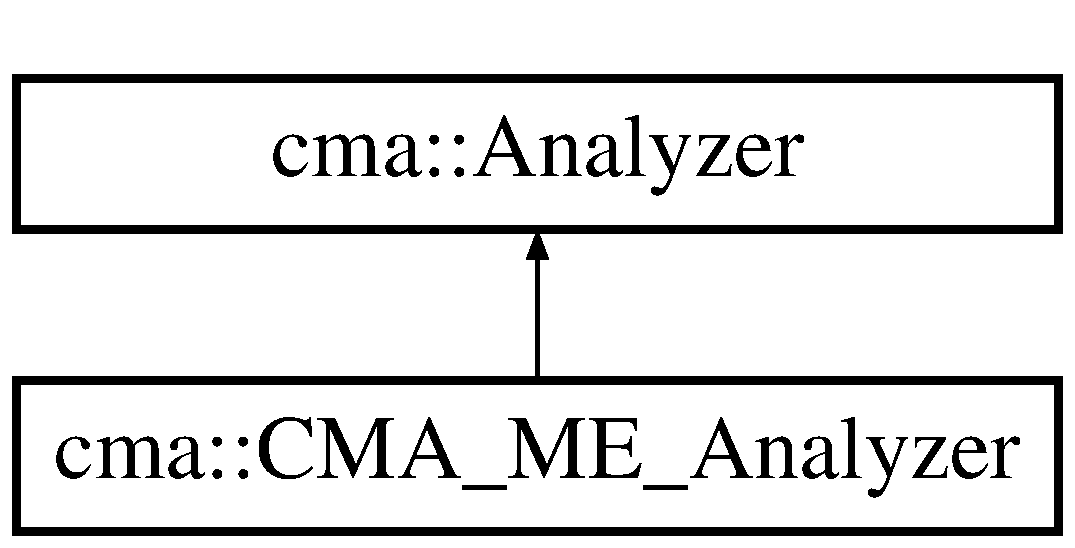
\includegraphics[height=2cm]{classcma_1_1Analyzer}
\end{center}
\end{figure}
\subsection*{Public Types}
\begin{CompactItemize}
\item 
enum {\bf OptionType} \{ {\bf OPTION\_\-TYPE\_\-POS\_\-TAGGING}, 
{\bf OPTION\_\-TYPE\_\-NBEST}, 
{\bf OPTION\_\-TYPE\_\-NUM}
 \}
\subsection*{Public Member Functions}
\begin{CompactItemize}
\item 
virtual void {\bf setKnowledge} ({\bf Knowledge} $\ast$pKnowledge)=0
\item 
virtual int {\bf runWithSentence} ({\bf Sentence} \&sentence)=0
\item 
virtual const char $\ast$ {\bf runWithString} (const char $\ast$inStr)=0
\item 
virtual int {\bf runWithStream} (const char $\ast$inFileName, const char $\ast$outFileName)=0
\item 
virtual void {\bf splitSentence} (const char $\ast$paragraph, std::vector$<$ {\bf Sentence} $>$ \&sentences)=0
\item 
void {\bf setOption} ({\bf OptionType} nOption, double nValue)
\item 
double {\bf getOption} ({\bf OptionType} nOption) const 
\item 
void {\bf setPOSDelimiter} (const char $\ast$delimiter)
\item 
const char $\ast$ {\bf getPOSDelimiter} () const 
\item 
void {\bf setWordDelimiter} (const char $\ast$delimiter)
\item 
const char $\ast$ {\bf getWordDelimiter} () const 
\end{CompactItemize}
\subsection*{Protected Attributes}
\begin{CompactItemize}
\item 
std::vector$<$ double $>$ {\bf options\_\-}
\item 
const char $\ast$ {\bf posDelimiter\_\-}
\item 
const char $\ast$ {\bf wordDelimiter\_\-}
\end{CompactItemize}


\subsection{Detailed Description}
\doxyref{Analyzer}{p.}{classcma_1_1Analyzer} executes the Chinese morphological analysis. 

\doxyref{Analyzer}{p.}{classcma_1_1Analyzer} executes the Chinese morphological analysis. Typically, the usage is like below:

// create instances CMA\_\-Factory$\ast$ factory = \doxyref{CMA\_\-Factory::instance()}{p.}{classcma_1_1CMA__Factory_9a7abf5a22bc6aefd6994e54ccd745b8}; Analyzer$\ast$ analyzer = factory-$>$createAnalyzer(); Knowledge$\ast$ knowledge = factory-$>$createKnowledge();

// load dictionaries knowledge-$>$loadSystemDict(\char`\"{}...\char`\"{}); knowledge-$>$loadUserDict(\char`\"{}...\char`\"{}); knowledge-$>$loadStopWordDict(\char`\"{}...\char`\"{}); knowledge-$>$loadStatModel(\char`\"{}...\char`\"{});

// set knowledge analyzer-$>$setKnowledge(knowledge);

// analyze a sentence \doxyref{Sentence}{p.}{classcma_1_1Sentence} s; s.setString(\char`\"{}...\char`\"{}); analyzer-$>$runWithSentence(s); ...

// analyze a paragraph const char$\ast$ result = analyzer-$>$runWithString(\char`\"{}...\char`\"{}); ...

// analyze a file analyzer-$>$runWithStream(\char`\"{}...\char`\"{}, \char`\"{}...\char`\"{});

delete knowledge; delete analyzer; 

\subsection{Member Enumeration Documentation}
\index{cma::Analyzer@{cma::Analyzer}!OptionType@{OptionType}}
\index{OptionType@{OptionType}!cma::Analyzer@{cma::Analyzer}}
\subsubsection[{OptionType}]{\setlength{\rightskip}{0pt plus 5cm}enum {\bf cma::Analyzer::OptionType}}\label{classcma_1_1Analyzer_828bd41bd7badd423d6cef5aa1454efe}


Option type for analysis. \begin{Desc}
\item[Enumerator: ]\par
\begin{description}
\index{OPTION\_\-TYPE\_\-POS\_\-TAGGING@{OPTION\_\-TYPE\_\-POS\_\-TAGGING}!cma::Analyzer@{cma::Analyzer}}\index{cma::Analyzer@{cma::Analyzer}!OPTION\_\-TYPE\_\-POS\_\-TAGGING@{OPTION\_\-TYPE\_\-POS\_\-TAGGING}}\item[{\em 
OPTION\_\-TYPE\_\-POS\_\-TAGGING\label{classcma_1_1Analyzer_828bd41bd7badd423d6cef5aa1454efee6788d85d45be70c6b72ddf9948b43b2}
}]the value zero for not to tag part-of-speech tags in the result of {\em \doxyref{runWithSentence()}{p.}{classcma_1_1Analyzer_2274acc45dd1ccc6aa7ea87cd34ad0e7}\/}, {\em \doxyref{runWithString()}{p.}{classcma_1_1Analyzer_2d05785e30e19a390aa887f25bda2d2f}\/} and {\em \doxyref{runWithStream()}{p.}{classcma_1_1Analyzer_ae19c787b296d086d52449cb1b6e3699}\/}, which value is 1 defaultly. \index{OPTION\_\-TYPE\_\-NBEST@{OPTION\_\-TYPE\_\-NBEST}!cma::Analyzer@{cma::Analyzer}}\index{cma::Analyzer@{cma::Analyzer}!OPTION\_\-TYPE\_\-NBEST@{OPTION\_\-TYPE\_\-NBEST}}\item[{\em 
OPTION\_\-TYPE\_\-NBEST\label{classcma_1_1Analyzer_828bd41bd7badd423d6cef5aa1454efe7737be8d0d08f661301fb1b90f0a96bc}
}]a positive value to set the number of candidate results of {\em \doxyref{runWithSentence()}{p.}{classcma_1_1Analyzer_2274acc45dd1ccc6aa7ea87cd34ad0e7}\/}, which value is 1 defaultly. \index{OPTION\_\-TYPE\_\-NUM@{OPTION\_\-TYPE\_\-NUM}!cma::Analyzer@{cma::Analyzer}}\index{cma::Analyzer@{cma::Analyzer}!OPTION\_\-TYPE\_\-NUM@{OPTION\_\-TYPE\_\-NUM}}\item[{\em 
OPTION\_\-TYPE\_\-NUM\label{classcma_1_1Analyzer_828bd41bd7badd423d6cef5aa1454efe2951e28fcefc2733d78dadcec45c15ac}
}]the count of option types \end{description}
\end{Desc}



\subsection{Member Function Documentation}
\index{cma::Analyzer@{cma::Analyzer}!getOption@{getOption}}
\index{getOption@{getOption}!cma::Analyzer@{cma::Analyzer}}
\subsubsection[{getOption}]{\setlength{\rightskip}{0pt plus 5cm}double cma::Analyzer::getOption ({\bf OptionType} {\em nOption}) const}\label{classcma_1_1Analyzer_8df9e86073a5e3d0f44dce0c14f27706}


Get the option value. \begin{Desc}
\item[Parameters:]
\begin{description}
\item[{\em nOption}]the option type \end{description}
\end{Desc}
\begin{Desc}
\item[Returns:]the option value \end{Desc}


References options\_\-.

Referenced by cma::CMA\_\-ME\_\-Analyzer::runWithSentence(), cma::CMA\_\-ME\_\-Analyzer::runWithStream(), and cma::CMA\_\-ME\_\-Analyzer::runWithString().\index{cma::Analyzer@{cma::Analyzer}!getPOSDelimiter@{getPOSDelimiter}}
\index{getPOSDelimiter@{getPOSDelimiter}!cma::Analyzer@{cma::Analyzer}}
\subsubsection[{getPOSDelimiter}]{\setlength{\rightskip}{0pt plus 5cm}const char $\ast$ cma::Analyzer::getPOSDelimiter () const}\label{classcma_1_1Analyzer_e5351b7f2fa7717b1b5af2be8a86c04f}


Get the delimiter between word and POS tag in the output result of {\em \doxyref{runWithString()}{p.}{classcma_1_1Analyzer_2d05785e30e19a390aa887f25bda2d2f}\/} and {\em \doxyref{runWithStream()}{p.}{classcma_1_1Analyzer_ae19c787b296d086d52449cb1b6e3699}\/}, which delimiter is \char`\"{}/\char`\"{} defaultly so that the result would be \char`\"{}word/pos  word/pos  ...\char`\"{}. \begin{Desc}
\item[Returns:]the delimiter between word and POS tag in the output result \end{Desc}


References posDelimiter\_\-.\index{cma::Analyzer@{cma::Analyzer}!getWordDelimiter@{getWordDelimiter}}
\index{getWordDelimiter@{getWordDelimiter}!cma::Analyzer@{cma::Analyzer}}
\subsubsection[{getWordDelimiter}]{\setlength{\rightskip}{0pt plus 5cm}const char $\ast$ cma::Analyzer::getWordDelimiter () const}\label{classcma_1_1Analyzer_bee23d91de22d6083c3ba41a126d43a6}


Get the delimiter between the pairs (word and POS tag) in the output result of {\em \doxyref{runWithString()}{p.}{classcma_1_1Analyzer_2d05785e30e19a390aa887f25bda2d2f}\/} and {\em \doxyref{runWithStream()}{p.}{classcma_1_1Analyzer_ae19c787b296d086d52449cb1b6e3699}\/}, which delimiter is \char`\"{}  \char`\"{} (double-space) defaultly so that the result would be \char`\"{}word/pos  word/pos  ...\char`\"{}. \begin{Desc}
\item[Returns:]the delimiter between the pairs (word and POS tag) in the output result \end{Desc}


References wordDelimiter\_\-.\index{cma::Analyzer@{cma::Analyzer}!runWithSentence@{runWithSentence}}
\index{runWithSentence@{runWithSentence}!cma::Analyzer@{cma::Analyzer}}
\subsubsection[{runWithSentence}]{\setlength{\rightskip}{0pt plus 5cm}virtual int cma::Analyzer::runWithSentence ({\bf Sentence} \& {\em sentence})\hspace{0.3cm}{\tt  [pure virtual]}}\label{classcma_1_1Analyzer_2274acc45dd1ccc6aa7ea87cd34ad0e7}


Execute the morphological analysis based on a sentence. \begin{Desc}
\item[Parameters:]
\begin{description}
\item[{\em sentence}]the instance containing the raw sentence string and also to save the analysis result \end{description}
\end{Desc}
\begin{Desc}
\item[Returns:]0 for fail, 1 for success \end{Desc}
\begin{Desc}
\item[Precondition:]the raw sentence string could be got by {\em sentence.getString()\/}. \end{Desc}
\begin{Desc}
\item[Postcondition:]on successful return, the n-best results could be got by {\em sentence.getListSize()\/}, etc. \end{Desc}


Implemented in {\bf cma::CMA\_\-ME\_\-Analyzer} \doxyref{}{p.}{classcma_1_1CMA__ME__Analyzer_6bac993f470b61cc4fccdbd4a7217948}.\index{cma::Analyzer@{cma::Analyzer}!runWithStream@{runWithStream}}
\index{runWithStream@{runWithStream}!cma::Analyzer@{cma::Analyzer}}
\subsubsection[{runWithStream}]{\setlength{\rightskip}{0pt plus 5cm}virtual int cma::Analyzer::runWithStream (const char $\ast$ {\em inFileName}, \/  const char $\ast$ {\em outFileName})\hspace{0.3cm}{\tt  [pure virtual]}}\label{classcma_1_1Analyzer_ae19c787b296d086d52449cb1b6e3699}


Execute the morphological analysis based on a file. \begin{Desc}
\item[Parameters:]
\begin{description}
\item[{\em inFileName}]input file name \item[{\em outFileName}]output file name \end{description}
\end{Desc}
\begin{Desc}
\item[Returns:]0 for fail, 1 for success \end{Desc}
\begin{Desc}
\item[Postcondition:]on successful return, the one-best result is printed to file {\em outFileName\/}. \end{Desc}


Implemented in {\bf cma::CMA\_\-ME\_\-Analyzer} \doxyref{}{p.}{classcma_1_1CMA__ME__Analyzer_eb9e065c3cc25885f2ccb0c70f4a5964}.

Referenced by beginSeg().\index{cma::Analyzer@{cma::Analyzer}!runWithString@{runWithString}}
\index{runWithString@{runWithString}!cma::Analyzer@{cma::Analyzer}}
\subsubsection[{runWithString}]{\setlength{\rightskip}{0pt plus 5cm}virtual const char$\ast$ cma::Analyzer::runWithString (const char $\ast$ {\em inStr})\hspace{0.3cm}{\tt  [pure virtual]}}\label{classcma_1_1Analyzer_2d05785e30e19a390aa887f25bda2d2f}


Execute the morphological analysis based on a paragraph string. \begin{Desc}
\item[Parameters:]
\begin{description}
\item[{\em inStr}]paragraph string \end{description}
\end{Desc}
\begin{Desc}
\item[Returns:]0 for fail, otherwise a non-zero string pointer for the one-best result \end{Desc}


Implemented in {\bf cma::CMA\_\-ME\_\-Analyzer} \doxyref{}{p.}{classcma_1_1CMA__ME__Analyzer_50b039c84be34cc7c83ce8aef97058f2}.\index{cma::Analyzer@{cma::Analyzer}!setKnowledge@{setKnowledge}}
\index{setKnowledge@{setKnowledge}!cma::Analyzer@{cma::Analyzer}}
\subsubsection[{setKnowledge}]{\setlength{\rightskip}{0pt plus 5cm}virtual void cma::Analyzer::setKnowledge ({\bf Knowledge} $\ast$ {\em pKnowledge})\hspace{0.3cm}{\tt  [pure virtual]}}\label{classcma_1_1Analyzer_52d2462f2f05cec4a9c4d6773e7502cb}


Set the {\em \doxyref{Knowledge}{p.}{classcma_1_1Knowledge}\/} for analysis. \begin{Desc}
\item[Parameters:]
\begin{description}
\item[{\em pKnowledge}]the pointer of {\em \doxyref{Knowledge}{p.}{classcma_1_1Knowledge}\/} \end{description}
\end{Desc}


Implemented in {\bf cma::CMA\_\-ME\_\-Analyzer} \doxyref{}{p.}{classcma_1_1CMA__ME__Analyzer_04d6b5c7b7dcd199c8e96a06afa5ea44}.

Referenced by beginSeg().\index{cma::Analyzer@{cma::Analyzer}!setOption@{setOption}}
\index{setOption@{setOption}!cma::Analyzer@{cma::Analyzer}}
\subsubsection[{setOption}]{\setlength{\rightskip}{0pt plus 5cm}void cma::Analyzer::setOption ({\bf OptionType} {\em nOption}, \/  double {\em nValue})}\label{classcma_1_1Analyzer_d461885573a34670730fcb7ebcd10d99}


Set the option value for analysis. \begin{Desc}
\item[Parameters:]
\begin{description}
\item[{\em nOption}]the option type \item[{\em nValue}]the option value \end{description}
\end{Desc}
\begin{Desc}
\item[Attention:]when {\em nOption\/} is {\em OPTION\_\-TYPE\_\-NBEST\/}, the invalid {\em nValue\/} less than 1 will take no effect. \end{Desc}


References OPTION\_\-TYPE\_\-NBEST, and options\_\-.

Referenced by beginSeg().\index{cma::Analyzer@{cma::Analyzer}!setPOSDelimiter@{setPOSDelimiter}}
\index{setPOSDelimiter@{setPOSDelimiter}!cma::Analyzer@{cma::Analyzer}}
\subsubsection[{setPOSDelimiter}]{\setlength{\rightskip}{0pt plus 5cm}void cma::Analyzer::setPOSDelimiter (const char $\ast$ {\em delimiter})}\label{classcma_1_1Analyzer_7c4b88bf29930661262f3c05be208471}


Set the delimiter between word and POS tag in the output result of {\em \doxyref{runWithString()}{p.}{classcma_1_1Analyzer_2d05785e30e19a390aa887f25bda2d2f}\/} and {\em \doxyref{runWithStream()}{p.}{classcma_1_1Analyzer_ae19c787b296d086d52449cb1b6e3699}\/}, which delimiter is \char`\"{}/\char`\"{} defaultly so that the result would be \char`\"{}word/pos  word/pos  ...\char`\"{}. \begin{Desc}
\item[Parameters:]
\begin{description}
\item[{\em delimiter}]the delimiter between word and POS tag in the output result \end{description}
\end{Desc}


References posDelimiter\_\-.

Referenced by beginSeg().\index{cma::Analyzer@{cma::Analyzer}!setWordDelimiter@{setWordDelimiter}}
\index{setWordDelimiter@{setWordDelimiter}!cma::Analyzer@{cma::Analyzer}}
\subsubsection[{setWordDelimiter}]{\setlength{\rightskip}{0pt plus 5cm}void cma::Analyzer::setWordDelimiter (const char $\ast$ {\em delimiter})}\label{classcma_1_1Analyzer_c9bba08c5455b6e640065e420d1974d7}


Set the delimiter between the pairs (word and POS tag) in the output result of {\em \doxyref{runWithString()}{p.}{classcma_1_1Analyzer_2d05785e30e19a390aa887f25bda2d2f}\/} and {\em \doxyref{runWithStream()}{p.}{classcma_1_1Analyzer_ae19c787b296d086d52449cb1b6e3699}\/}, which delimiter is \char`\"{}  \char`\"{} (double-space) defaultly so that the result would be \char`\"{}word/pos  word/pos  ...\char`\"{}. \begin{Desc}
\item[Parameters:]
\begin{description}
\item[{\em delimiter}]the delimiter between the pairs (word and POS tag) in the output result \end{description}
\end{Desc}


References wordDelimiter\_\-.\index{cma::Analyzer@{cma::Analyzer}!splitSentence@{splitSentence}}
\index{splitSentence@{splitSentence}!cma::Analyzer@{cma::Analyzer}}
\subsubsection[{splitSentence}]{\setlength{\rightskip}{0pt plus 5cm}virtual void cma::Analyzer::splitSentence (const char $\ast$ {\em paragraph}, \/  std::vector$<$ {\bf Sentence} $>$ \& {\em sentences})\hspace{0.3cm}{\tt  [pure virtual]}}\label{classcma_1_1Analyzer_8ed5115519284c1ccf2bde9e289168dd}


Split a paragraph string into sentences. \begin{Desc}
\item[Parameters:]
\begin{description}
\item[{\em paragraph}]paragraph string \item[{\em sentences}]sentence vector \end{description}
\end{Desc}
\begin{Desc}
\item[Attention:]the original elements in {\em sentences\/} would not be removed, and the splited sentences are appended into {\em sentences\/}. \end{Desc}


Implemented in {\bf cma::CMA\_\-ME\_\-Analyzer} \doxyref{}{p.}{classcma_1_1CMA__ME__Analyzer_b6d7b5e169207cca37337eceb07ac5fe}.

\subsection{Member Data Documentation}
\index{cma::Analyzer@{cma::Analyzer}!options\_\-@{options\_\-}}
\index{options\_\-@{options\_\-}!cma::Analyzer@{cma::Analyzer}}
\subsubsection[{options\_\-}]{\setlength{\rightskip}{0pt plus 5cm}std::vector$<$double$>$ {\bf cma::Analyzer::options\_\-}\hspace{0.3cm}{\tt  [protected]}}\label{classcma_1_1Analyzer_e48091098a6b1e544ef3ac5517b5d1cc}


option values 

Referenced by getOption(), and setOption().\index{cma::Analyzer@{cma::Analyzer}!posDelimiter\_\-@{posDelimiter\_\-}}
\index{posDelimiter\_\-@{posDelimiter\_\-}!cma::Analyzer@{cma::Analyzer}}
\subsubsection[{posDelimiter\_\-}]{\setlength{\rightskip}{0pt plus 5cm}const char$\ast$ {\bf cma::Analyzer::posDelimiter\_\-}\hspace{0.3cm}{\tt  [protected]}}\label{classcma_1_1Analyzer_3649af9da4b6022fd9761ab59bb249c2}


the delimiter between word and POS tag in the output result 

Referenced by getPOSDelimiter(), cma::CMA\_\-ME\_\-Analyzer::runWithStream(), cma::CMA\_\-ME\_\-Analyzer::runWithString(), and setPOSDelimiter().\index{cma::Analyzer@{cma::Analyzer}!wordDelimiter\_\-@{wordDelimiter\_\-}}
\index{wordDelimiter\_\-@{wordDelimiter\_\-}!cma::Analyzer@{cma::Analyzer}}
\subsubsection[{wordDelimiter\_\-}]{\setlength{\rightskip}{0pt plus 5cm}const char$\ast$ {\bf cma::Analyzer::wordDelimiter\_\-}\hspace{0.3cm}{\tt  [protected]}}\label{classcma_1_1Analyzer_2bc9276661a6c732dc52dbc3fda74817}


the delimiter between the pairs (word and POS tag) in the output result 

Referenced by getWordDelimiter(), cma::CMA\_\-ME\_\-Analyzer::runWithStream(), cma::CMA\_\-ME\_\-Analyzer::runWithString(), and setWordDelimiter().

The documentation for this class was generated from the following files:\begin{CompactItemize}
\item 
include/{\bf analyzer.h}\item 
source/src/{\bf analyzer.cpp}\end{CompactItemize}

\section{cma::CatePoint Struct Reference}
\label{structcma_1_1CatePoint}\index{cma::CatePoint@{cma::CatePoint}}
Record the index and category of the specific index.  


{\tt \#include $<$CateStrTokenizer.h$>$}

\subsection*{Public Attributes}
\begin{CompactItemize}
\item 
int {\bf index}
\item 
CharType {\bf type}
\end{CompactItemize}


\subsection{Detailed Description}
Record the index and category of the specific index. 

Record the index and category of the specific index 

\subsection{Member Data Documentation}
\index{cma::CatePoint@{cma::CatePoint}!index@{index}}
\index{index@{index}!cma::CatePoint@{cma::CatePoint}}
\subsubsection[{index}]{\setlength{\rightskip}{0pt plus 5cm}int {\bf cma::CatePoint::index}}\label{structcma_1_1CatePoint_4d5fb8b0c7028e57ef179c0630f0eee7}


The index in the whole string \index{cma::CatePoint@{cma::CatePoint}!type@{type}}
\index{type@{type}!cma::CatePoint@{cma::CatePoint}}
\subsubsection[{type}]{\setlength{\rightskip}{0pt plus 5cm}CharType {\bf cma::CatePoint::type}}\label{structcma_1_1CatePoint_1eddb8c6760d5cd21d5f15b1ee8eb01f}


Three Type: Letter/Digit/Punctuation 

The documentation for this struct was generated from the following file:\begin{CompactItemize}
\item 
source/include/{\bf CateStrTokenizer.h}\end{CompactItemize}

\section{cma::CMA\_\-CType Class Reference}
\label{classcma_1_1CMA__CType}\index{cma::CMA\_\-CType@{cma::CMA\_\-CType}}
\doxyref{CMA\_\-CType}{p.}{classcma_1_1CMA__CType} gives the character type information.  


{\tt \#include $<$cma\_\-ctype.h$>$}

Inheritance diagram for cma::CMA\_\-CType::\begin{figure}[H]
\begin{center}
\leavevmode
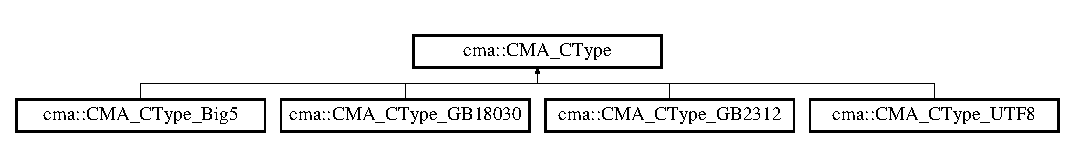
\includegraphics[height=2cm]{classcma_1_1CMA__CType}
\end{center}
\end{figure}
\subsection*{Public Member Functions}
\begin{CompactItemize}
\item 
virtual {\bf $\sim$CMA\_\-CType} ()
\item 
virtual unsigned int {\bf getByteCount} (const char $\ast$p) const =0
\item 
virtual CharType {\bf getCharType} (const char $\ast$p, CharType preType, const char $\ast$nextP) const =0
\item 
bool {\bf isPunct} (const char $\ast$p) const 
\item 
size\_\-t {\bf length} (const char $\ast$p) const 
\end{CompactItemize}
\subsection*{Static Public Member Functions}
\begin{CompactItemize}
\item 
static {\bf CMA\_\-CType} $\ast$ {\bf instance} ({\bf Knowledge::EncodeType} type)
\item 
static {\bf Knowledge::EncodeType} {\bf getEncType} (string encType)
\end{CompactItemize}


\subsection{Detailed Description}
\doxyref{CMA\_\-CType}{p.}{classcma_1_1CMA__CType} gives the character type information. 

\doxyref{CMA\_\-CType}{p.}{classcma_1_1CMA__CType} gives the character type information. 

\subsection{Constructor \& Destructor Documentation}
\index{cma::CMA\_\-CType@{cma::CMA\_\-CType}!$\sim$CMA\_\-CType@{$\sim$CMA\_\-CType}}
\index{$\sim$CMA\_\-CType@{$\sim$CMA\_\-CType}!cma::CMA_CType@{cma::CMA\_\-CType}}
\subsubsection{\setlength{\rightskip}{0pt plus 5cm}cma::CMA\_\-CType::$\sim$CMA\_\-CType ()\hspace{0.3cm}{\tt  [virtual]}}\label{classcma_1_1CMA__CType_a5069cd1dc6794e4744e3fbcac7afbd6}


Destrucor 

\subsection{Member Function Documentation}
\index{cma::CMA\_\-CType@{cma::CMA\_\-CType}!instance@{instance}}
\index{instance@{instance}!cma::CMA_CType@{cma::CMA\_\-CType}}
\subsubsection{\setlength{\rightskip}{0pt plus 5cm}{\bf CMA\_\-CType} $\ast$ cma::CMA\_\-CType::instance ({\bf Knowledge::EncodeType} {\em type})\hspace{0.3cm}{\tt  [static]}}\label{classcma_1_1CMA__CType_a0a1b4e5959587032b22036c64790314}


Create an instance of {\em \doxyref{CMA\_\-CType}{p.}{classcma_1_1CMA__CType}\/} based on the character encode type. \begin{Desc}
\item[Parameters:]
\begin{description}
\item[{\em type}]the character encode type \end{description}
\end{Desc}
\begin{Desc}
\item[Returns:]the pointer to instance \end{Desc}


References cma::Knowledge::ENCODE\_\-TYPE\_\-BIG5, cma::Knowledge::ENCODE\_\-TYPE\_\-GB2312, cma::CMA\_\-CType\_\-Big5::instance(), and cma::CMA\_\-CType\_\-GB2312::instance().

Referenced by cma::CMA\_\-ME\_\-Analyzer::setKnowledge().\index{cma::CMA\_\-CType@{cma::CMA\_\-CType}!getEncType@{getEncType}}
\index{getEncType@{getEncType}!cma::CMA_CType@{cma::CMA\_\-CType}}
\subsubsection{\setlength{\rightskip}{0pt plus 5cm}{\bf Knowledge::EncodeType} cma::CMA\_\-CType::getEncType (string {\em encType})\hspace{0.3cm}{\tt  [static]}}\label{classcma_1_1CMA__CType_2a912dfae4c56e70a20f920ac564890b}


Get the encoding type by the encode type string

\begin{Desc}
\item[Parameters:]
\begin{description}
\item[{\em encType}]encode type string \end{description}
\end{Desc}
\begin{Desc}
\item[Returns:]assicated \doxyref{Knowledge::EncodeType}{p.}{classcma_1_1Knowledge_2f725921dec755cdd496e81a95389f1d} in the class \doxyref{Knowledge}{p.}{classcma_1_1Knowledge} \end{Desc}


References cma::Knowledge::ENCODE\_\-TYPE\_\-BIG5, cma::Knowledge::ENCODE\_\-TYPE\_\-GB2312, and cma::Knowledge::ENCODE\_\-TYPE\_\-NUM.\index{cma::CMA\_\-CType@{cma::CMA\_\-CType}!getByteCount@{getByteCount}}
\index{getByteCount@{getByteCount}!cma::CMA_CType@{cma::CMA\_\-CType}}
\subsubsection{\setlength{\rightskip}{0pt plus 5cm}virtual unsigned int cma::CMA\_\-CType::getByteCount (const char $\ast$ {\em p}) const\hspace{0.3cm}{\tt  [pure virtual]}}\label{classcma_1_1CMA__CType_00f7e99cea12e9db504629c4a6cdb2d4}


Get the byte count of the first character pointed by {\em p\/}, which character is in a specific encoding. \begin{Desc}
\item[Parameters:]
\begin{description}
\item[{\em p}]pointer to the character string \end{description}
\end{Desc}
\begin{Desc}
\item[Returns:]true for punctuation, false for non punctuation. \end{Desc}


Implemented in {\bf cma::CMA\_\-CType\_\-Big5} \doxyref{}{p.}{classcma_1_1CMA__CType__Big5_0e471b0985214eb074b69fe273cde7f5}, and {\bf cma::CMA\_\-CType\_\-GB2312} \doxyref{}{p.}{classcma_1_1CMA__CType__GB2312_057ccee8e82b0a22a30b79fb2f059b8f}.

Referenced by length(), and cma::CTypeTokenizer::next().\index{cma::CMA\_\-CType@{cma::CMA\_\-CType}!getCharType@{getCharType}}
\index{getCharType@{getCharType}!cma::CMA_CType@{cma::CMA\_\-CType}}
\subsubsection{\setlength{\rightskip}{0pt plus 5cm}virtual CharType cma::CMA\_\-CType::getCharType (const char $\ast$ {\em p}, \/  CharType {\em preType}, \/  const char $\ast$ {\em nextP}) const\hspace{0.3cm}{\tt  [pure virtual]}}\label{classcma_1_1CMA__CType_45412869e7ededc53dcc432d43d6a025}


Get the character type. \begin{Desc}
\item[Parameters:]
\begin{description}
\item[{\em p}]pointer to the string to be checked \item[{\em preType}]the chartype of the previous character \item[{\em nextP}]the pointer of the next character, it can be 0 \end{description}
\end{Desc}
\begin{Desc}
\item[Returns:]the character type. \end{Desc}


Implemented in {\bf cma::CMA\_\-CType\_\-Big5} \doxyref{}{p.}{classcma_1_1CMA__CType__Big5_a125ef224739df73781aa6ee55d28b38}, and {\bf cma::CMA\_\-CType\_\-GB2312} \doxyref{}{p.}{classcma_1_1CMA__CType__GB2312_e0edf1c74d7a66ba6425b9010401456e}.

Referenced by cma::CMA\_\-WType::getWordType(), isPunct(), and cma::CateStrTokenizer::next().\index{cma::CMA\_\-CType@{cma::CMA\_\-CType}!isPunct@{isPunct}}
\index{isPunct@{isPunct}!cma::CMA_CType@{cma::CMA\_\-CType}}
\subsubsection{\setlength{\rightskip}{0pt plus 5cm}bool cma::CMA\_\-CType::isPunct (const char $\ast$ {\em p}) const}\label{classcma_1_1CMA__CType_b9fbb6aa32fd36bb3838b48ffb92bf24}


Whether the p is a punctuation \begin{Desc}
\item[Parameters:]
\begin{description}
\item[{\em p}]pointer to the string to be checked \end{description}
\end{Desc}
\begin{Desc}
\item[Returns:]true if the p is the punctuation \end{Desc}


References getCharType().\index{cma::CMA\_\-CType@{cma::CMA\_\-CType}!length@{length}}
\index{length@{length}!cma::CMA_CType@{cma::CMA\_\-CType}}
\subsubsection{\setlength{\rightskip}{0pt plus 5cm}size\_\-t cma::CMA\_\-CType::length (const char $\ast$ {\em p}) const}\label{classcma_1_1CMA__CType_4583d638f7336cf0a548905e8e88f826}


Get the number of the characters in the p \begin{Desc}
\item[Parameters:]
\begin{description}
\item[{\em p}]pointer to the string to be checked \end{description}
\end{Desc}
\begin{Desc}
\item[Returns:]the number of the characters in the p \end{Desc}


References getByteCount().

The documentation for this class was generated from the following files:\begin{CompactItemize}
\item 
source/include/{\bf cma\_\-ctype.h}\item 
source/src/{\bf cma\_\-ctype.cpp}\end{CompactItemize}

\section{cma::CMA\_\-CType\_\-Big5 Class Reference}
\label{classcma_1_1CMA__CType__Big5}\index{cma::CMA\_\-CType\_\-Big5@{cma::CMA\_\-CType\_\-Big5}}
\doxyref{CMA\_\-CType\_\-Big5}{p.}{classcma_1_1CMA__CType__Big5} gives the character type information in Big5 encoding.  


{\tt \#include $<$cma\_\-ctype\_\-big5.h$>$}

Inheritance diagram for cma::CMA\_\-CType\_\-Big5::\begin{figure}[H]
\begin{center}
\leavevmode
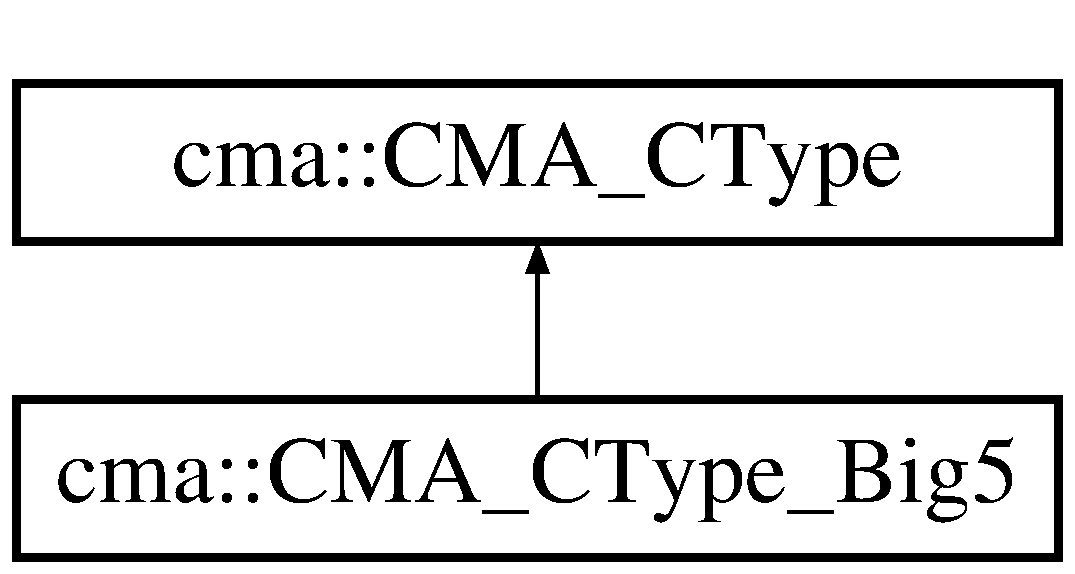
\includegraphics[height=2cm]{classcma_1_1CMA__CType__Big5}
\end{center}
\end{figure}
\subsection*{Public Member Functions}
\begin{CompactItemize}
\item 
virtual unsigned int {\bf getByteCount} (const char $\ast$p) const 
\item 
virtual CharType {\bf getCharType} (const char $\ast$p, CharType preType, const char $\ast$nextP) const 
\end{CompactItemize}
\subsection*{Static Public Member Functions}
\begin{CompactItemize}
\item 
static {\bf CMA\_\-CType\_\-Big5} $\ast$ {\bf instance} ()
\end{CompactItemize}
\subsection*{Protected Member Functions}
\begin{CompactItemize}
\item 
{\bf CMA\_\-CType\_\-Big5} ()
\end{CompactItemize}


\subsection{Detailed Description}
\doxyref{CMA\_\-CType\_\-Big5}{p.}{classcma_1_1CMA__CType__Big5} gives the character type information in Big5 encoding. 

\subsection{Constructor \& Destructor Documentation}
\index{cma::CMA\_\-CType\_\-Big5@{cma::CMA\_\-CType\_\-Big5}!CMA\_\-CType\_\-Big5@{CMA\_\-CType\_\-Big5}}
\index{CMA\_\-CType\_\-Big5@{CMA\_\-CType\_\-Big5}!cma::CMA_CType_Big5@{cma::CMA\_\-CType\_\-Big5}}
\subsubsection[{CMA\_\-CType\_\-Big5}]{\setlength{\rightskip}{0pt plus 5cm}cma::CMA\_\-CType\_\-Big5::CMA\_\-CType\_\-Big5 ()\hspace{0.3cm}{\tt  [protected]}}\label{classcma_1_1CMA__CType__Big5_6363b4086243edf9fa7ea68b80b677ed}


Avoid invoked directly 

\subsection{Member Function Documentation}
\index{cma::CMA\_\-CType\_\-Big5@{cma::CMA\_\-CType\_\-Big5}!getByteCount@{getByteCount}}
\index{getByteCount@{getByteCount}!cma::CMA_CType_Big5@{cma::CMA\_\-CType\_\-Big5}}
\subsubsection[{getByteCount}]{\setlength{\rightskip}{0pt plus 5cm}unsigned int cma::CMA\_\-CType\_\-Big5::getByteCount (const char $\ast$ {\em p}) const\hspace{0.3cm}{\tt  [virtual]}}\label{classcma_1_1CMA__CType__Big5_0e471b0985214eb074b69fe273cde7f5}


Get the byte count of the first character pointed by {\em p\/}, which character is in a specific encoding. \begin{Desc}
\item[Parameters:]
\begin{description}
\item[{\em p}]pointer to the character string \end{description}
\end{Desc}
\begin{Desc}
\item[Returns:]the count of bytes. \end{Desc}


Implements {\bf cma::CMA\_\-CType} \doxyref{}{p.}{classcma_1_1CMA__CType_00f7e99cea12e9db504629c4a6cdb2d4}.\index{cma::CMA\_\-CType\_\-Big5@{cma::CMA\_\-CType\_\-Big5}!getCharType@{getCharType}}
\index{getCharType@{getCharType}!cma::CMA_CType_Big5@{cma::CMA\_\-CType\_\-Big5}}
\subsubsection[{getCharType}]{\setlength{\rightskip}{0pt plus 5cm}CharType cma::CMA\_\-CType\_\-Big5::getCharType (const char $\ast$ {\em p}, \/  CharType {\em preType}, \/  const char $\ast$ {\em nextP}) const\hspace{0.3cm}{\tt  [virtual]}}\label{classcma_1_1CMA__CType__Big5_a125ef224739df73781aa6ee55d28b38}


Get the character type. \begin{Desc}
\item[Parameters:]
\begin{description}
\item[{\em p}]pointer to the string to be checked \item[{\em preType}]the chartype of the previous character \item[{\em nextP}]the pointer of the next character, it can be 0 \end{description}
\end{Desc}
\begin{Desc}
\item[Returns:]the character type. \end{Desc}


Implements {\bf cma::CMA\_\-CType} \doxyref{}{p.}{classcma_1_1CMA__CType_45412869e7ededc53dcc432d43d6a025}.\index{cma::CMA\_\-CType\_\-Big5@{cma::CMA\_\-CType\_\-Big5}!instance@{instance}}
\index{instance@{instance}!cma::CMA_CType_Big5@{cma::CMA\_\-CType\_\-Big5}}
\subsubsection[{instance}]{\setlength{\rightskip}{0pt plus 5cm}{\bf CMA\_\-CType\_\-Big5} $\ast$ cma::CMA\_\-CType\_\-Big5::instance ()\hspace{0.3cm}{\tt  [static]}}\label{classcma_1_1CMA__CType__Big5_ac103ebf44d2a2d35aef04312c064235}


Create an instance of {\em \doxyref{CMA\_\-CType\_\-Big5}{p.}{classcma_1_1CMA__CType__Big5}\/}. \begin{Desc}
\item[Returns:]the pointer to instance \end{Desc}


The documentation for this class was generated from the following files:\begin{CompactItemize}
\item 
source/include/{\bf cma\_\-ctype\_\-big5.h}\item 
source/src/{\bf cma\_\-ctype\_\-big5.cpp}\end{CompactItemize}

\section{cma::CMA\_\-CType\_\-GB2312 Class Reference}
\label{classcma_1_1CMA__CType__GB2312}\index{cma::CMA\_\-CType\_\-GB2312@{cma::CMA\_\-CType\_\-GB2312}}


\doxyref{CMA\_\-CType\_\-GB2312}{p.}{classcma_1_1CMA__CType__GB2312} gives the character type information in GB2312 encoding.  


{\ttfamily \#include $<$cma\_\-ctype\_\-gb2312.h$>$}Inheritance diagram for cma::CMA\_\-CType\_\-GB2312::\begin{figure}[H]
\begin{center}
\leavevmode
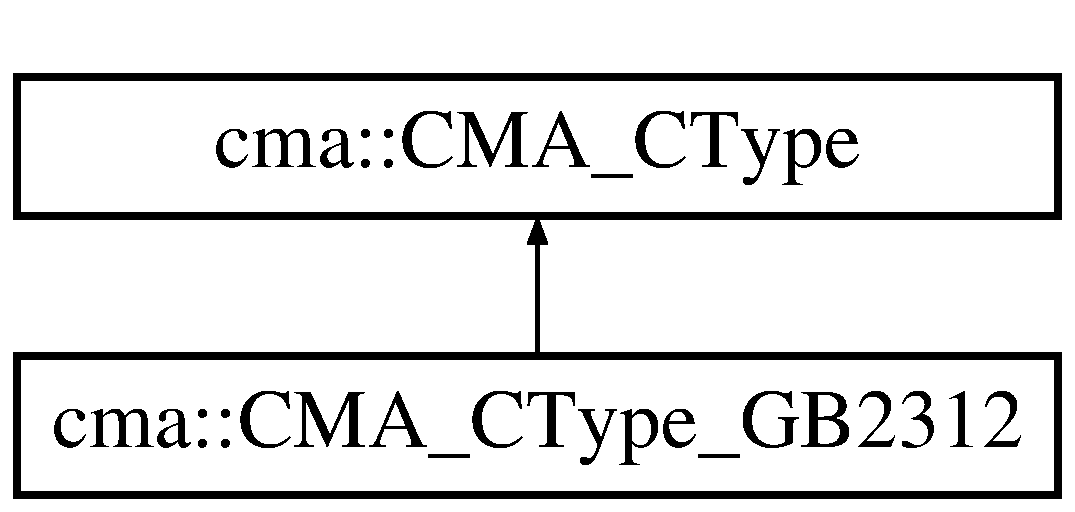
\includegraphics[height=2cm]{classcma_1_1CMA__CType__GB2312}
\end{center}
\end{figure}
\subsection*{Public Member Functions}
\begin{DoxyCompactItemize}
\item 
virtual unsigned int {\bf getByteCount} (const char $\ast$p) const 
\end{DoxyCompactItemize}
\subsection*{Static Public Member Functions}
\begin{DoxyCompactItemize}
\item 
static {\bf CMA\_\-CType\_\-GB2312} $\ast$ {\bf instance} ()
\end{DoxyCompactItemize}
\subsection*{Protected Member Functions}
\begin{DoxyCompactItemize}
\item 
{\bf CMA\_\-CType\_\-GB2312} ()
\end{DoxyCompactItemize}


\subsection{Detailed Description}
\doxyref{CMA\_\-CType\_\-GB2312}{p.}{classcma_1_1CMA__CType__GB2312} gives the character type information in GB2312 encoding. 

\subsection{Constructor \& Destructor Documentation}
\index{cma::CMA\_\-CType\_\-GB2312@{cma::CMA\_\-CType\_\-GB2312}!CMA\_\-CType\_\-GB2312@{CMA\_\-CType\_\-GB2312}}
\index{CMA\_\-CType\_\-GB2312@{CMA\_\-CType\_\-GB2312}!cma::CMA_CType_GB2312@{cma::CMA\_\-CType\_\-GB2312}}
\subsubsection[{CMA\_\-CType\_\-GB2312}]{\setlength{\rightskip}{0pt plus 5cm}cma::CMA\_\-CType\_\-GB2312::CMA\_\-CType\_\-GB2312 ()\hspace{0.3cm}{\ttfamily  [protected]}}\label{classcma_1_1CMA__CType__GB2312_a74352ef545209d1b8fd55fac0bf515c0}
Get the character type. 
\begin{DoxyParams}{Parameters}
\item[{\em p}]pointer to the string to be checked \item[{\em preType}]the chartype of the previous character \item[{\em nextP}]the pointer of the next character, it can be 0 \end{DoxyParams}
\begin{DoxyReturn}{Returns}
the character type. Check whether is white-\/space character. White-\/space characters are \char`\"{} $\backslash$t$\backslash$n$\backslash$v$\backslash$f$\backslash$r\char`\"{}, and also space character in specific encoding. 
\end{DoxyReturn}

\begin{DoxyParams}{Parameters}
\item[{\em p}]pointer to the character string \end{DoxyParams}
\begin{DoxyReturn}{Returns}
true for white-\/space character, false for non white-\/space character. Check whether is a separator of sentence. 
\end{DoxyReturn}

\begin{DoxyParams}{Parameters}
\item[{\em p}]pointer to the character string \end{DoxyParams}
\begin{DoxyReturn}{Returns}
true for separator, false for non separator. Avoid invoked directly 
\end{DoxyReturn}


References cma::Knowledge::ENCODE\_\-TYPE\_\-GB2312, and cma::CMA\_\-CType::type\_\-.

\subsection{Member Function Documentation}
\index{cma::CMA\_\-CType\_\-GB2312@{cma::CMA\_\-CType\_\-GB2312}!getByteCount@{getByteCount}}
\index{getByteCount@{getByteCount}!cma::CMA_CType_GB2312@{cma::CMA\_\-CType\_\-GB2312}}
\subsubsection[{getByteCount}]{\setlength{\rightskip}{0pt plus 5cm}unsigned int cma::CMA\_\-CType\_\-GB2312::getByteCount (const char $\ast$ {\em p}) const\hspace{0.3cm}{\ttfamily  [virtual]}}\label{classcma_1_1CMA__CType__GB2312_a057ccee8e82b0a22a30b79fb2f059b8f}
Get the byte count of the first character pointed by {\itshape p\/}, which character is in a specific encoding. 
\begin{DoxyParams}{Parameters}
\item[{\em p}]pointer to the character string \end{DoxyParams}
\begin{DoxyReturn}{Returns}
the count of bytes. 
\end{DoxyReturn}


Implements {\bf cma::CMA\_\-CType} \doxyref{}{p.}{classcma_1_1CMA__CType_a00f7e99cea12e9db504629c4a6cdb2d4}.\index{cma::CMA\_\-CType\_\-GB2312@{cma::CMA\_\-CType\_\-GB2312}!instance@{instance}}
\index{instance@{instance}!cma::CMA_CType_GB2312@{cma::CMA\_\-CType\_\-GB2312}}
\subsubsection[{instance}]{\setlength{\rightskip}{0pt plus 5cm}{\bf CMA\_\-CType\_\-GB2312} $\ast$ cma::CMA\_\-CType\_\-GB2312::instance ()\hspace{0.3cm}{\ttfamily  [static]}}\label{classcma_1_1CMA__CType__GB2312_af34c920bf4afbc1a764f97e8b8b6e8cd}
Create an instance of {\itshape \doxyref{CMA\_\-CType\_\-GB2312}{p.}{classcma_1_1CMA__CType__GB2312}\/}. \begin{DoxyReturn}{Returns}
the pointer to instance 
\end{DoxyReturn}


The documentation for this class was generated from the following files:\begin{DoxyCompactItemize}
\item 
/home/vernkin/projects/chinese-\/ma-\/chen/source/include/{\bf cma\_\-ctype\_\-gb2312.h}\item 
/home/vernkin/projects/chinese-\/ma-\/chen/source/src/{\bf cma\_\-ctype\_\-gb2312.cpp}\end{DoxyCompactItemize}

\section{cma::CMA\_\-Factory Class Reference}
\label{classcma_1_1CMA__Factory}\index{cma::CMA\_\-Factory@{cma::CMA\_\-Factory}}


\doxyref{CMA\_\-Factory}{p.}{classcma_1_1CMA__Factory} creates instances for Chinese morphological analysis.  


{\ttfamily \#include $<$cma\_\-factory.h$>$}Inheritance diagram for cma::CMA\_\-Factory::\begin{figure}[H]
\begin{center}
\leavevmode
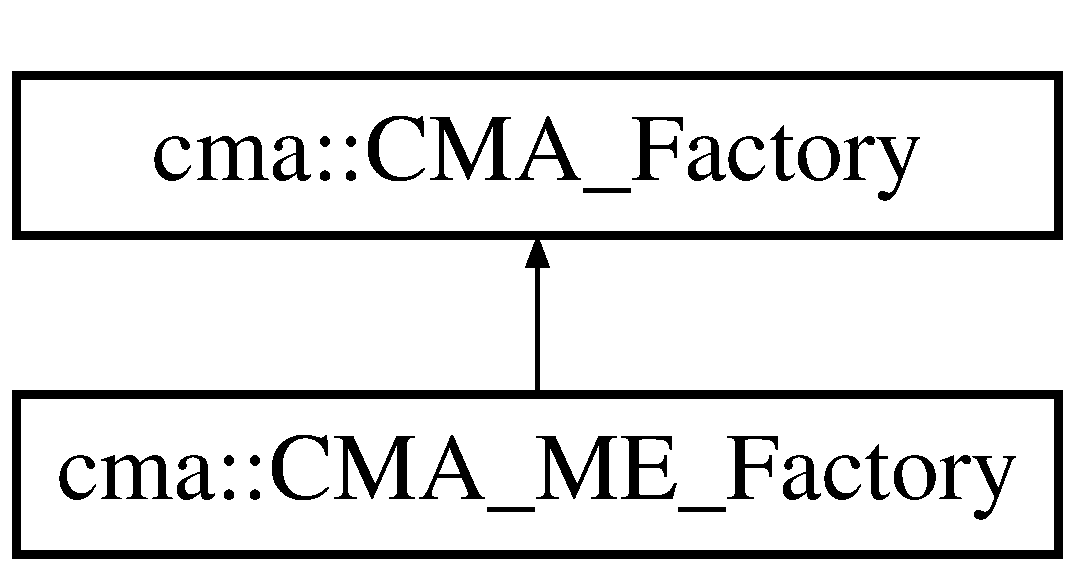
\includegraphics[height=2cm]{classcma_1_1CMA__Factory}
\end{center}
\end{figure}
\subsection*{Public Member Functions}
\begin{DoxyCompactItemize}
\item 
virtual {\bf Analyzer} $\ast$ {\bf createAnalyzer} ()=0
\item 
virtual {\bf Knowledge} $\ast$ {\bf createKnowledge} ()=0
\end{DoxyCompactItemize}
\subsection*{Static Public Member Functions}
\begin{DoxyCompactItemize}
\item 
static {\bf CMA\_\-Factory} $\ast$ {\bf instance} ()
\end{DoxyCompactItemize}


\subsection{Detailed Description}
\doxyref{CMA\_\-Factory}{p.}{classcma_1_1CMA__Factory} creates instances for Chinese morphological analysis. 

\subsection{Member Function Documentation}
\index{cma::CMA\_\-Factory@{cma::CMA\_\-Factory}!createAnalyzer@{createAnalyzer}}
\index{createAnalyzer@{createAnalyzer}!cma::CMA_Factory@{cma::CMA\_\-Factory}}
\subsubsection[{createAnalyzer}]{\setlength{\rightskip}{0pt plus 5cm}virtual {\bf Analyzer}$\ast$ cma::CMA\_\-Factory::createAnalyzer ()\hspace{0.3cm}{\ttfamily  [pure virtual]}}\label{classcma_1_1CMA__Factory_a8657bc77b2eae6520cbae0526d0434e9}
Create an instance of {\itshape \doxyref{Analyzer}{p.}{classcma_1_1Analyzer}\/}. \begin{DoxyReturn}{Returns}
the pointer to instance 
\end{DoxyReturn}


Implemented in {\bf cma::CMA\_\-ME\_\-Factory} \doxyref{}{p.}{classcma_1_1CMA__ME__Factory_ae315f718993b56cd9c884f10e2247da7}.

Referenced by beginSeg().\index{cma::CMA\_\-Factory@{cma::CMA\_\-Factory}!createKnowledge@{createKnowledge}}
\index{createKnowledge@{createKnowledge}!cma::CMA_Factory@{cma::CMA\_\-Factory}}
\subsubsection[{createKnowledge}]{\setlength{\rightskip}{0pt plus 5cm}virtual {\bf Knowledge}$\ast$ cma::CMA\_\-Factory::createKnowledge ()\hspace{0.3cm}{\ttfamily  [pure virtual]}}\label{classcma_1_1CMA__Factory_aa5d13d8795c258566d87782ada486214}
Create an instance of {\itshape \doxyref{Knowledge}{p.}{classcma_1_1Knowledge}\/}. \begin{DoxyReturn}{Returns}
the pointer to instance 
\end{DoxyReturn}


Implemented in {\bf cma::CMA\_\-ME\_\-Factory} \doxyref{}{p.}{classcma_1_1CMA__ME__Factory_a2a967832c088306b7c281c8bc3927555}.

Referenced by beginSeg().\index{cma::CMA\_\-Factory@{cma::CMA\_\-Factory}!instance@{instance}}
\index{instance@{instance}!cma::CMA_Factory@{cma::CMA\_\-Factory}}
\subsubsection[{instance}]{\setlength{\rightskip}{0pt plus 5cm}{\bf CMA\_\-Factory} $\ast$ cma::CMA\_\-Factory::instance ()\hspace{0.3cm}{\ttfamily  [static]}}\label{classcma_1_1CMA__Factory_a9a7abf5a22bc6aefd6994e54ccd745b8}
Create an instance of {\itshape \doxyref{CMA\_\-Factory}{p.}{classcma_1_1CMA__Factory}\/}. \begin{DoxyReturn}{Returns}
the pointer to instance 
\end{DoxyReturn}


The documentation for this class was generated from the following files:\begin{DoxyCompactItemize}
\item 
/home/vernkin/projects/chinese-\/ma-\/chen/include/{\bf cma\_\-factory.h}\item 
/home/vernkin/projects/chinese-\/ma-\/chen/source/src/{\bf cma\_\-factory.cpp}\end{DoxyCompactItemize}

\section{cma::CMA\_\-ME\_\-Analyzer Class Reference}
\label{classcma_1_1CMA__ME__Analyzer}\index{cma::CMA\_\-ME\_\-Analyzer@{cma::CMA\_\-ME\_\-Analyzer}}


\doxyref{Analyzer}{p.}{classcma_1_1Analyzer} for the CMAC.  


{\ttfamily \#include $<$CMA\_\-ME\_\-Analyzer.h$>$}Inheritance diagram for cma::CMA\_\-ME\_\-Analyzer::\begin{figure}[H]
\begin{center}
\leavevmode
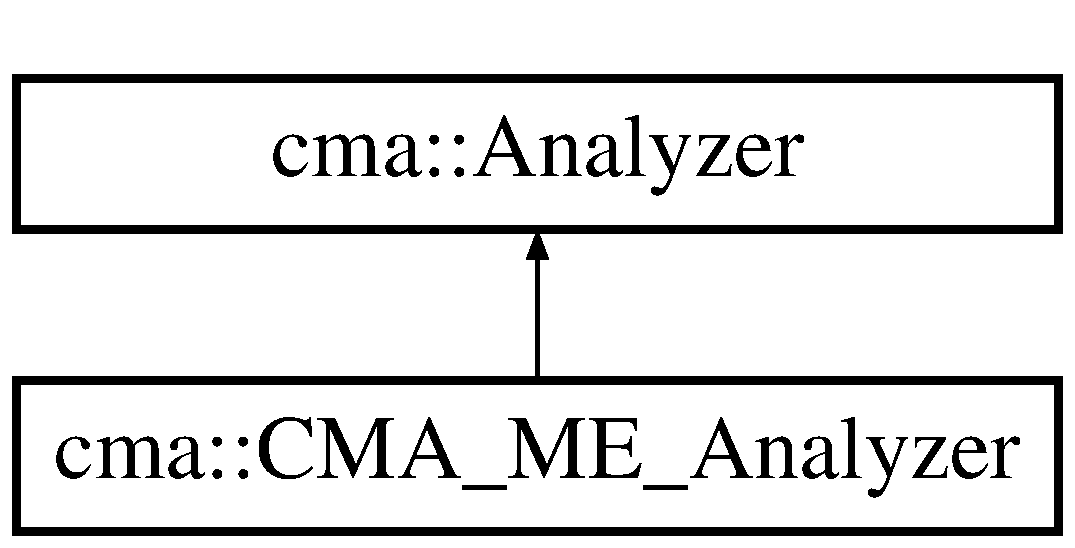
\includegraphics[height=2cm]{classcma_1_1CMA__ME__Analyzer}
\end{center}
\end{figure}
\subsection*{Public Types}
\begin{DoxyCompactItemize}
\item 
typedef string {\bfseries OneGramType}\label{classcma_1_1CMA__ME__Analyzer_a9b615fa3994c626a039187c7444ba0f0}

\end{DoxyCompactItemize}
\subsection*{Public Member Functions}
\begin{DoxyCompactItemize}
\item 
{\bf $\sim$CMA\_\-ME\_\-Analyzer} ()
\item 
virtual void {\bf setKnowledge} ({\bf Knowledge} $\ast$pKnowledge)
\item 
virtual int {\bf runWithSentence} ({\bf Sentence} \&sentence)
\item 
virtual const char $\ast$ {\bf runWithString} (const char $\ast$inStr)
\item 
virtual int {\bf runWithStream} (const char $\ast$inFileName, const char $\ast$outFileName)
\item 
virtual void {\bf getNGramResult} (const char $\ast$inStr, int n, vector$<$ string $>$ \&output)
\item 
virtual void {\bf getNGramArrayResult} (const char $\ast$inStr, vector$<$ int $>$ nArray, vector$<$ string $>$ \&output)
\item 
virtual void {\bf splitSentence} (const char $\ast$paragraph, std::vector$<$ {\bf Sentence} $>$ \&sentences)
\item 
virtual void {\bf resetIndexPOSList} (bool defVal=true)
\item 
virtual int {\bf setIndexPOSList} (std::vector$<$ std::string $>$ \&posList)
\item 
virtual int {\bf getCodeFromStr} (const std::string \&pos) const 
\item 
virtual const char $\ast$ {\bf getStrFromCode} (int index) const 
\item 
virtual int {\bf getPOSTagSetSize} () const 
\end{DoxyCompactItemize}


\subsection{Detailed Description}
\doxyref{Analyzer}{p.}{classcma_1_1Analyzer} for the CMAC. 

\subsection{Constructor \& Destructor Documentation}
\index{cma::CMA\_\-ME\_\-Analyzer@{cma::CMA\_\-ME\_\-Analyzer}!$\sim$CMA\_\-ME\_\-Analyzer@{$\sim$CMA\_\-ME\_\-Analyzer}}
\index{$\sim$CMA\_\-ME\_\-Analyzer@{$\sim$CMA\_\-ME\_\-Analyzer}!cma::CMA_ME_Analyzer@{cma::CMA\_\-ME\_\-Analyzer}}
\subsubsection[{$\sim$CMA\_\-ME\_\-Analyzer}]{\setlength{\rightskip}{0pt plus 5cm}cma::CMA\_\-ME\_\-Analyzer::$\sim$CMA\_\-ME\_\-Analyzer ()}\label{classcma_1_1CMA__ME__Analyzer_a67e7728f4fa010deaa8f30c575e0c078}
The Desconstrutor won't delete knowledge pointer 

\subsection{Member Function Documentation}
\index{cma::CMA\_\-ME\_\-Analyzer@{cma::CMA\_\-ME\_\-Analyzer}!getCodeFromStr@{getCodeFromStr}}
\index{getCodeFromStr@{getCodeFromStr}!cma::CMA_ME_Analyzer@{cma::CMA\_\-ME\_\-Analyzer}}
\subsubsection[{getCodeFromStr}]{\setlength{\rightskip}{0pt plus 5cm}virtual int cma::CMA\_\-ME\_\-Analyzer::getCodeFromStr (const std::string \& {\em pos}) const\hspace{0.3cm}{\ttfamily  [virtual]}}\label{classcma_1_1CMA__ME__Analyzer_a51f3d3d9df1f88de445740aa56aab336}
Get the POS index code from the POS string in the global part-\/of-\/speech table. 
\begin{DoxyParams}{Parameters}
\item[{\em pos}]the POS string \end{DoxyParams}
\begin{DoxyReturn}{Returns}
POS index code, -\/1 for non POS available 
\end{DoxyReturn}


Implements {\bf cma::Analyzer} \doxyref{}{p.}{classcma_1_1Analyzer_a8cf23f3e17a8d808ab946e2a6474d08b}.\index{cma::CMA\_\-ME\_\-Analyzer@{cma::CMA\_\-ME\_\-Analyzer}!getNGramArrayResult@{getNGramArrayResult}}
\index{getNGramArrayResult@{getNGramArrayResult}!cma::CMA_ME_Analyzer@{cma::CMA\_\-ME\_\-Analyzer}}
\subsubsection[{getNGramArrayResult}]{\setlength{\rightskip}{0pt plus 5cm}void cma::CMA\_\-ME\_\-Analyzer::getNGramArrayResult (const char $\ast$ {\em inStr}, \/  vector$<$ int $>$ {\em nArray}, \/  vector$<$ string $>$ \& {\em output})\hspace{0.3cm}{\ttfamily  [virtual]}}\label{classcma_1_1CMA__ME__Analyzer_a9b9ed98bd9782764d866f94145b9bf65}
Get all the specific N-\/Gram results (see parameter nArray) in the inStr 
\begin{DoxyParams}{Parameters}
\item[{\em inStr}]paragraph string \item[{\em nArray}]the collection of the specific n in the N-\/Gram \item[{\em output}]to keep the output value \end{DoxyParams}
\index{cma::CMA\_\-ME\_\-Analyzer@{cma::CMA\_\-ME\_\-Analyzer}!getNGramResult@{getNGramResult}}
\index{getNGramResult@{getNGramResult}!cma::CMA_ME_Analyzer@{cma::CMA\_\-ME\_\-Analyzer}}
\subsubsection[{getNGramResult}]{\setlength{\rightskip}{0pt plus 5cm}void cma::CMA\_\-ME\_\-Analyzer::getNGramResult (const char $\ast$ {\em inStr}, \/  int {\em n}, \/  vector$<$ string $>$ \& {\em output})\hspace{0.3cm}{\ttfamily  [virtual]}}\label{classcma_1_1CMA__ME__Analyzer_a590bac470ef26b7935f26aec808919f1}
Get the N-\/Gram result in the inStr 
\begin{DoxyParams}{Parameters}
\item[{\em inStr}]paragraph string \item[{\em n}]the specific n in the N-\/Gram \item[{\em output}]to keep the output value \end{DoxyParams}
\index{cma::CMA\_\-ME\_\-Analyzer@{cma::CMA\_\-ME\_\-Analyzer}!getPOSTagSetSize@{getPOSTagSetSize}}
\index{getPOSTagSetSize@{getPOSTagSetSize}!cma::CMA_ME_Analyzer@{cma::CMA\_\-ME\_\-Analyzer}}
\subsubsection[{getPOSTagSetSize}]{\setlength{\rightskip}{0pt plus 5cm}int cma::CMA\_\-ME\_\-Analyzer::getPOSTagSetSize () const\hspace{0.3cm}{\ttfamily  [virtual]}}\label{classcma_1_1CMA__ME__Analyzer_a6defaeb4b7ce84d3688ce9d42fde2145}
Get the number of POS tags in the global part-\/of-\/speech table. \begin{DoxyReturn}{Returns}
the number of POS tags 
\end{DoxyReturn}


Implements {\bf cma::Analyzer} \doxyref{}{p.}{classcma_1_1Analyzer_a5607a772d430d7e2923d29720f5aa63a}.

References cma::POSTable::size().\index{cma::CMA\_\-ME\_\-Analyzer@{cma::CMA\_\-ME\_\-Analyzer}!getStrFromCode@{getStrFromCode}}
\index{getStrFromCode@{getStrFromCode}!cma::CMA_ME_Analyzer@{cma::CMA\_\-ME\_\-Analyzer}}
\subsubsection[{getStrFromCode}]{\setlength{\rightskip}{0pt plus 5cm}const char $\ast$ cma::CMA\_\-ME\_\-Analyzer::getStrFromCode (int {\em index}) const\hspace{0.3cm}{\ttfamily  [virtual]}}\label{classcma_1_1CMA__ME__Analyzer_a05d471db9b5c1cccdebb9a21582acaad}
Get the POS string from the POS index code in the global part-\/of-\/speech table. 
\begin{DoxyParams}{Parameters}
\item[{\em index}]the POS index code \end{DoxyParams}
\begin{DoxyReturn}{Returns}
POS string, null pointer for non POS available 
\end{DoxyReturn}


Implements {\bf cma::Analyzer} \doxyref{}{p.}{classcma_1_1Analyzer_a2ba8615ba11be2409aa80b62ad1f7a1b}.

References cma::POSTable::getStrFromCode().\index{cma::CMA\_\-ME\_\-Analyzer@{cma::CMA\_\-ME\_\-Analyzer}!resetIndexPOSList@{resetIndexPOSList}}
\index{resetIndexPOSList@{resetIndexPOSList}!cma::CMA_ME_Analyzer@{cma::CMA\_\-ME\_\-Analyzer}}
\subsubsection[{resetIndexPOSList}]{\setlength{\rightskip}{0pt plus 5cm}void cma::CMA\_\-ME\_\-Analyzer::resetIndexPOSList (bool {\em defVal} = {\ttfamily true})\hspace{0.3cm}{\ttfamily  [virtual]}}\label{classcma_1_1CMA__ME__Analyzer_afa513b05898ec374781c5889ed9714c8}
Reset all the POS index Information as defVal \begin{DoxyReturn}{Returns}
defVal default value to reset (default is true) 
\end{DoxyReturn}


Implements {\bf cma::Analyzer} \doxyref{}{p.}{classcma_1_1Analyzer_a4e2aad23b33ceeb60265dd68daf9da67}.

References cma::POSTable::resetIndexPOSList().\index{cma::CMA\_\-ME\_\-Analyzer@{cma::CMA\_\-ME\_\-Analyzer}!runWithSentence@{runWithSentence}}
\index{runWithSentence@{runWithSentence}!cma::CMA_ME_Analyzer@{cma::CMA\_\-ME\_\-Analyzer}}
\subsubsection[{runWithSentence}]{\setlength{\rightskip}{0pt plus 5cm}int cma::CMA\_\-ME\_\-Analyzer::runWithSentence ({\bf Sentence} \& {\em sentence})\hspace{0.3cm}{\ttfamily  [virtual]}}\label{classcma_1_1CMA__ME__Analyzer_a6bac993f470b61cc4fccdbd4a7217948}
Execute the morphological analysis based on a sentence. 
\begin{DoxyParams}{Parameters}
\item[{\em sentence}]an instance of {\itshape \doxyref{Sentence}{p.}{classcma_1_1Sentence}\/} \end{DoxyParams}
\begin{DoxyReturn}{Returns}
0 for fail, 1 for success 
\end{DoxyReturn}
\begin{DoxyPrecond}{Precondition}
the raw sentence string could be got by {\itshape sentence.getString()\/}. 
\end{DoxyPrecond}
\begin{DoxyPostcond}{Postcondition}
on successful return, the n-\/best results could be got by {\itshape sentence.getListSize()\/}, etc. 
\end{DoxyPostcond}
\begin{DoxyAttention}{Attention}
white-\/space characters are ignored in the analysis, which include \char`\"{} $\backslash$t$\backslash$n$\backslash$v$\backslash$f$\backslash$r\char`\"{}, and also space character in specific encoding. 
\end{DoxyAttention}


Implements {\bf cma::Analyzer} \doxyref{}{p.}{classcma_1_1Analyzer_a2274acc45dd1ccc6aa7ea87cd34ad0e7}.

References cma::Sentence::addList(), cma::POSTable::getCodeFromStr(), cma::Sentence::getListSize(), cma::Sentence::getMorphemeList(), cma::Analyzer::getOption(), cma::Sentence::getScore(), cma::Sentence::getString(), cma::Morpheme::isIndexed, cma::POSTable::isIndexPOS(), cma::CMA\_\-ME\_\-Knowledge::isStopWord(), cma::Morpheme::lexicon\_\-, cma::Analyzer::OPTION\_\-TYPE\_\-NBEST, cma::Analyzer::OPTION\_\-TYPE\_\-POS\_\-TAGGING, cma::Morpheme::posCode\_\-, cma::Morpheme::posStr\_\-, and cma::Sentence::setScore().\index{cma::CMA\_\-ME\_\-Analyzer@{cma::CMA\_\-ME\_\-Analyzer}!runWithStream@{runWithStream}}
\index{runWithStream@{runWithStream}!cma::CMA_ME_Analyzer@{cma::CMA\_\-ME\_\-Analyzer}}
\subsubsection[{runWithStream}]{\setlength{\rightskip}{0pt plus 5cm}int cma::CMA\_\-ME\_\-Analyzer::runWithStream (const char $\ast$ {\em inFileName}, \/  const char $\ast$ {\em outFileName})\hspace{0.3cm}{\ttfamily  [virtual]}}\label{classcma_1_1CMA__ME__Analyzer_aeb9e065c3cc25885f2ccb0c70f4a5964}
Execute the morphological analysis based on a file. 
\begin{DoxyParams}{Parameters}
\item[{\em inFileName}]input file name \item[{\em outFileName}]output file name \end{DoxyParams}
\begin{DoxyReturn}{Returns}
0 for fail, 1 for success 
\end{DoxyReturn}
\begin{DoxyPostcond}{Postcondition}
on successful return, the one-\/best result is printed to file {\itshape outFileName\/}. 
\end{DoxyPostcond}


Implements {\bf cma::Analyzer} \doxyref{}{p.}{classcma_1_1Analyzer_aae19c787b296d086d52449cb1b6e3699}.

References cma::Analyzer::getOption(), cma::CMA\_\-ME\_\-Knowledge::isStopWord(), cma::Analyzer::OPTION\_\-TYPE\_\-POS\_\-TAGGING, cma::Analyzer::posDelimiter\_\-, cma::Analyzer::sentenceDelimiter\_\-, and cma::Analyzer::wordDelimiter\_\-.\index{cma::CMA\_\-ME\_\-Analyzer@{cma::CMA\_\-ME\_\-Analyzer}!runWithString@{runWithString}}
\index{runWithString@{runWithString}!cma::CMA_ME_Analyzer@{cma::CMA\_\-ME\_\-Analyzer}}
\subsubsection[{runWithString}]{\setlength{\rightskip}{0pt plus 5cm}const char $\ast$ cma::CMA\_\-ME\_\-Analyzer::runWithString (const char $\ast$ {\em inStr})\hspace{0.3cm}{\ttfamily  [virtual]}}\label{classcma_1_1CMA__ME__Analyzer_a50b039c84be34cc7c83ce8aef97058f2}
Execute the morphological analysis based on a paragraph string. 
\begin{DoxyParams}{Parameters}
\item[{\em inStr}]paragraph string \end{DoxyParams}
\begin{DoxyReturn}{Returns}
0 for fail, otherwise a non-\/zero string pointer for the one-\/best result 
\end{DoxyReturn}


Implements {\bf cma::Analyzer} \doxyref{}{p.}{classcma_1_1Analyzer_a2d05785e30e19a390aa887f25bda2d2f}.

References cma::Analyzer::getOption(), cma::CMA\_\-ME\_\-Knowledge::isStopWord(), cma::Analyzer::OPTION\_\-TYPE\_\-POS\_\-TAGGING, cma::Analyzer::posDelimiter\_\-, and cma::Analyzer::wordDelimiter\_\-.\index{cma::CMA\_\-ME\_\-Analyzer@{cma::CMA\_\-ME\_\-Analyzer}!setIndexPOSList@{setIndexPOSList}}
\index{setIndexPOSList@{setIndexPOSList}!cma::CMA_ME_Analyzer@{cma::CMA\_\-ME\_\-Analyzer}}
\subsubsection[{setIndexPOSList}]{\setlength{\rightskip}{0pt plus 5cm}int cma::CMA\_\-ME\_\-Analyzer::setIndexPOSList (std::vector$<$ std::string $>$ \& {\em posList})\hspace{0.3cm}{\ttfamily  [virtual]}}\label{classcma_1_1CMA__ME__Analyzer_a523e50a8c933c9dbc78ddd137666a666}
Set the POS index as true in the posList 
\begin{DoxyParams}{Parameters}
\item[{\em posList}]the list that allowed in the posList \end{DoxyParams}
\begin{DoxyReturn}{Returns}
how many POS are set successfully (mainly because not exists). 
\end{DoxyReturn}


Implements {\bf cma::Analyzer} \doxyref{}{p.}{classcma_1_1Analyzer_a3f4726b064b1197f069e2505ef093720}.

References cma::POSTable::setIndexPOSList().\index{cma::CMA\_\-ME\_\-Analyzer@{cma::CMA\_\-ME\_\-Analyzer}!setKnowledge@{setKnowledge}}
\index{setKnowledge@{setKnowledge}!cma::CMA_ME_Analyzer@{cma::CMA\_\-ME\_\-Analyzer}}
\subsubsection[{setKnowledge}]{\setlength{\rightskip}{0pt plus 5cm}void cma::CMA\_\-ME\_\-Analyzer::setKnowledge ({\bf Knowledge} $\ast$ {\em pKnowledge})\hspace{0.3cm}{\ttfamily  [virtual]}}\label{classcma_1_1CMA__ME__Analyzer_a04d6b5c7b7dcd199c8e96a06afa5ea44}
Set the {\itshape \doxyref{Knowledge}{p.}{classcma_1_1Knowledge}\/} for analysis. 
\begin{DoxyParams}{Parameters}
\item[{\em pKnowledge}]the pointer of {\itshape \doxyref{Knowledge}{p.}{classcma_1_1Knowledge}\/} \end{DoxyParams}


Implements {\bf cma::Analyzer} \doxyref{}{p.}{classcma_1_1Analyzer_a52d2462f2f05cec4a9c4d6773e7502cb}.

References cma::Knowledge::getEncodeType(), cma::CMA\_\-ME\_\-Knowledge::getPOSTable(), cma::CMA\_\-ME\_\-Knowledge::getPOSTagger(), cma::CMA\_\-ME\_\-Knowledge::getSegTagger(), cma::CMA\_\-ME\_\-Knowledge::getSystemProperty(), cma::CMA\_\-CType::instance(), cma::CMA\_\-ME\_\-Knowledge::isSupportPOS(), cma::Analyzer::OPTION\_\-TYPE\_\-POS\_\-TAGGING, cma::POSTagger::setCType(), cma::Analyzer::setOption(), cma::Analyzer::setPOSDelimiter(), cma::Analyzer::setSentenceDelimiter(), and cma::Analyzer::setWordDelimiter().\index{cma::CMA\_\-ME\_\-Analyzer@{cma::CMA\_\-ME\_\-Analyzer}!splitSentence@{splitSentence}}
\index{splitSentence@{splitSentence}!cma::CMA_ME_Analyzer@{cma::CMA\_\-ME\_\-Analyzer}}
\subsubsection[{splitSentence}]{\setlength{\rightskip}{0pt plus 5cm}void cma::CMA\_\-ME\_\-Analyzer::splitSentence (const char $\ast$ {\em paragraph}, \/  std::vector$<$ {\bf Sentence} $>$ \& {\em sentences})\hspace{0.3cm}{\ttfamily  [virtual]}}\label{classcma_1_1CMA__ME__Analyzer_ab6d7b5e169207cca37337eceb07ac5fe}
Split a paragraph string into sentences. 
\begin{DoxyParams}{Parameters}
\item[{\em paragraph}]paragraph string \item[{\em sentences}]sentence vector \end{DoxyParams}
\begin{DoxyAttention}{Attention}
the original elements in {\itshape sentences\/} would not be removed, and the splited sentences are appended into {\itshape sentences\/}. 
\end{DoxyAttention}


Implements {\bf cma::Analyzer} \doxyref{}{p.}{classcma_1_1Analyzer_a8ed5115519284c1ccf2bde9e289168dd}.

References cma::CTypeTokenizer::assign(), cma::CMA\_\-CType::isSentenceSeparator(), cma::CMA\_\-CType::isSpace(), cma::CTypeTokenizer::next(), and cma::Sentence::setString().

The documentation for this class was generated from the following files:\begin{DoxyCompactItemize}
\item 
/home/vernkin/projects/chinese-\/ma-\/chen/source/include/{\bf CMA\_\-ME\_\-Analyzer.h}\item 
/home/vernkin/projects/chinese-\/ma-\/chen/source/src/{\bf CMA\_\-ME\_\-Analyzer.cc}\end{DoxyCompactItemize}

\section{cma::CMA\_\-ME\_\-Factory Class Reference}
\label{classcma_1_1CMA__ME__Factory}\index{cma::CMA\_\-ME\_\-Factory@{cma::CMA\_\-ME\_\-Factory}}
\doxyref{CMA\_\-ME\_\-Factory}{p.}{classcma_1_1CMA__ME__Factory} creates instances for Chinese morphological analysis.  


{\tt \#include $<$CMA\_\-ME\_\-Factory.h$>$}

Inheritance diagram for cma::CMA\_\-ME\_\-Factory::\begin{figure}[H]
\begin{center}
\leavevmode
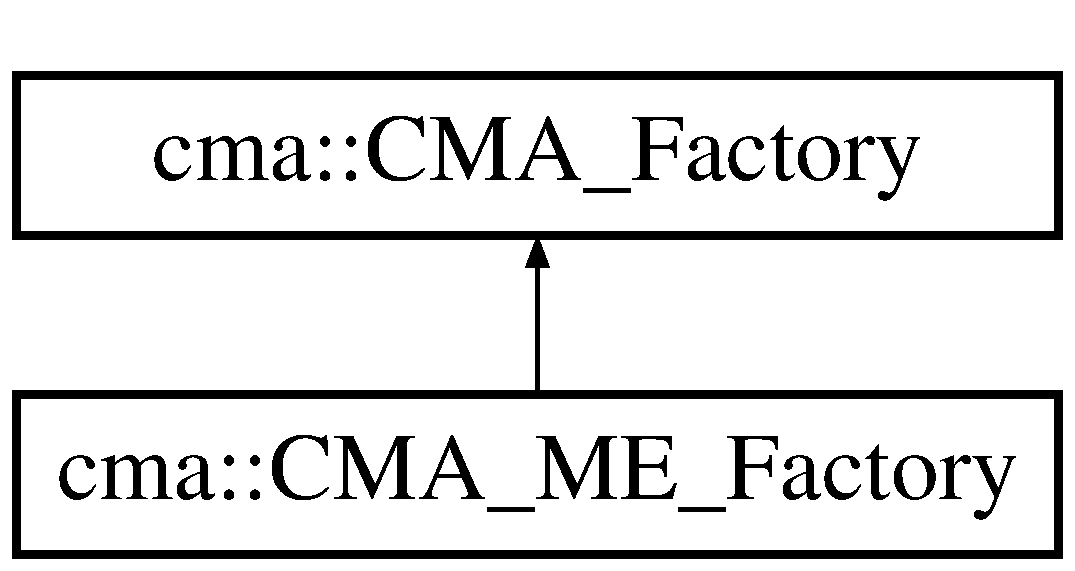
\includegraphics[height=2cm]{classcma_1_1CMA__ME__Factory}
\end{center}
\end{figure}
\subsection*{Public Member Functions}
\begin{CompactItemize}
\item 
virtual {\bf Analyzer} $\ast$ {\bf createAnalyzer} ()
\item 
virtual {\bf Knowledge} $\ast$ {\bf createKnowledge} ()
\end{CompactItemize}


\subsection{Detailed Description}
\doxyref{CMA\_\-ME\_\-Factory}{p.}{classcma_1_1CMA__ME__Factory} creates instances for Chinese morphological analysis. 

\subsection{Member Function Documentation}
\index{cma::CMA\_\-ME\_\-Factory@{cma::CMA\_\-ME\_\-Factory}!createAnalyzer@{createAnalyzer}}
\index{createAnalyzer@{createAnalyzer}!cma::CMA_ME_Factory@{cma::CMA\_\-ME\_\-Factory}}
\subsubsection[{createAnalyzer}]{\setlength{\rightskip}{0pt plus 5cm}{\bf Analyzer} $\ast$ cma::CMA\_\-ME\_\-Factory::createAnalyzer ()\hspace{0.3cm}{\tt  [virtual]}}\label{classcma_1_1CMA__ME__Factory_e315f718993b56cd9c884f10e2247da7}


Create an instance of {\em \doxyref{Analyzer}{p.}{classcma_1_1Analyzer}\/}. \begin{Desc}
\item[Returns:]the pointer to instance \end{Desc}


Implements {\bf cma::CMA\_\-Factory} \doxyref{}{p.}{classcma_1_1CMA__Factory_8657bc77b2eae6520cbae0526d0434e9}.\index{cma::CMA\_\-ME\_\-Factory@{cma::CMA\_\-ME\_\-Factory}!createKnowledge@{createKnowledge}}
\index{createKnowledge@{createKnowledge}!cma::CMA_ME_Factory@{cma::CMA\_\-ME\_\-Factory}}
\subsubsection[{createKnowledge}]{\setlength{\rightskip}{0pt plus 5cm}{\bf Knowledge} $\ast$ cma::CMA\_\-ME\_\-Factory::createKnowledge ()\hspace{0.3cm}{\tt  [virtual]}}\label{classcma_1_1CMA__ME__Factory_2a967832c088306b7c281c8bc3927555}


Create an instance of {\em \doxyref{Knowledge}{p.}{classcma_1_1Knowledge}\/}. \begin{Desc}
\item[Returns:]the pointer to instance \end{Desc}


Implements {\bf cma::CMA\_\-Factory} \doxyref{}{p.}{classcma_1_1CMA__Factory_a5d13d8795c258566d87782ada486214}.

The documentation for this class was generated from the following files:\begin{CompactItemize}
\item 
/home/vernkin/projects/chinese-ma-chen/source/include/{\bf CMA\_\-ME\_\-Factory.h}\item 
/home/vernkin/projects/chinese-ma-chen/source/src/{\bf CMA\_\-ME\_\-Factory.cc}\end{CompactItemize}

\section{cma::CMA\_\-ME\_\-Knowledge Class Reference}
\label{classcma_1_1CMA__ME__Knowledge}\index{cma::CMA\_\-ME\_\-Knowledge@{cma::CMA\_\-ME\_\-Knowledge}}
\doxyref{Knowledge}{p.}{classcma_1_1Knowledge} for the CMAC.  


{\tt \#include $<$CMA\_\-ME\_\-Knowledge.h$>$}

Inheritance diagram for cma::CMA\_\-ME\_\-Knowledge::\begin{figure}[H]
\begin{center}
\leavevmode
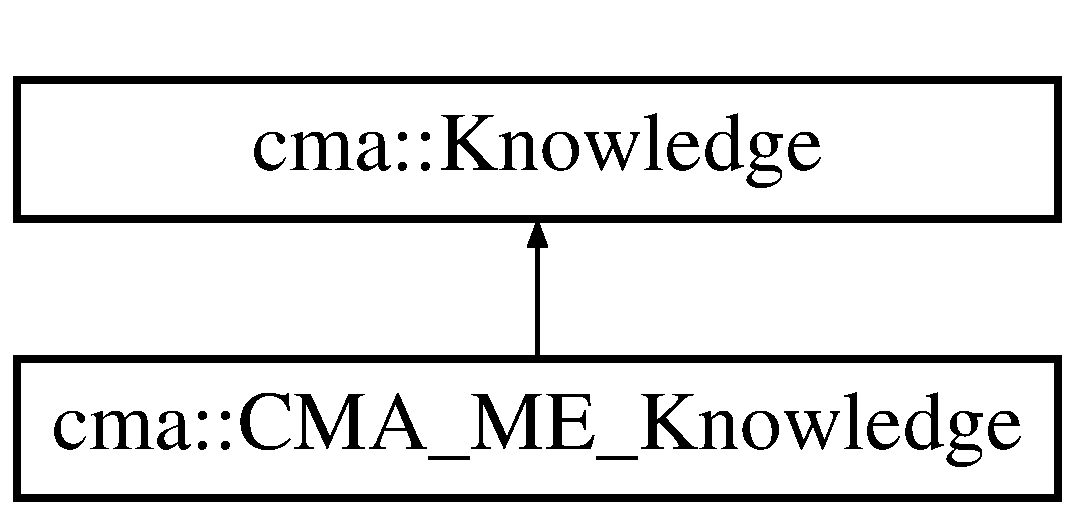
\includegraphics[height=2cm]{classcma_1_1CMA__ME__Knowledge}
\end{center}
\end{figure}
\subsection*{Public Member Functions}
\begin{CompactItemize}
\item 
virtual int {\bf loadSystemDict} (const char $\ast$binFileName)
\item 
virtual int {\bf loadUserDict} (const char $\ast$fileName)
\item 
virtual int {\bf loadSynonymDictionary} (const char $\ast$fileName)
\item 
virtual void {\bf getSynonyms} (const string \&word, {\bf VSynonym} \&synonym)
\item 
virtual int {\bf loadStopWordDict} (const char $\ast$fileName)
\item 
virtual int {\bf loadStatModel} (const char $\ast$cateName)
\item 
virtual int {\bf loadPOSModel} (const char $\ast$cateName)
\item 
virtual int {\bf loadConfig} (const char $\ast$fileName)
\item 
virtual int {\bf encodeSystemDict} (const char $\ast$txtFileName, const char $\ast$binFileName)
\item 
virtual int {\bf loadModel} (const char $\ast$encoding, const char $\ast$modelPath)
\item 
virtual bool {\bf isSupportPOS} () const 
\item 
{\bf SegTagger} $\ast$ {\bf getSegTagger} () const 
\item 
{\bf POSTagger} $\ast$ {\bf getPOSTagger} () const 
\item 
bool {\bf isStopWord} (const string \&word)
\item 
{\bf VTrie} $\ast$ {\bf getTrie} ()
\item 
const {\bf POSTable} $\ast$ {\bf getPOSTable} () const 
\item 
const string $\ast$ {\bf getSystemProperty} (const string \&key)
\end{CompactItemize}


\subsection{Detailed Description}
\doxyref{Knowledge}{p.}{classcma_1_1Knowledge} for the CMAC. 

\subsection{Member Function Documentation}
\index{cma::CMA\_\-ME\_\-Knowledge@{cma::CMA\_\-ME\_\-Knowledge}!encodeSystemDict@{encodeSystemDict}}
\index{encodeSystemDict@{encodeSystemDict}!cma::CMA_ME_Knowledge@{cma::CMA\_\-ME\_\-Knowledge}}
\subsubsection[{encodeSystemDict}]{\setlength{\rightskip}{0pt plus 5cm}int cma::CMA\_\-ME\_\-Knowledge::encodeSystemDict (const char $\ast$ {\em txtFileName}, \/  const char $\ast$ {\em binFileName})\hspace{0.3cm}{\tt  [virtual]}}\label{classcma_1_1CMA__ME__Knowledge_578eab67c328dcde77c359f54cb6557f}


Encode the system dictionary file from text to binary format. \begin{Desc}
\item[Parameters:]
\begin{description}
\item[{\em txtFileName}]the text file name \item[{\em binFileName}]the binary file name \end{description}
\end{Desc}
\begin{Desc}
\item[Returns:]0 for fail, 1 for success \end{Desc}


Implements {\bf cma::Knowledge} \doxyref{}{p.}{classcma_1_1Knowledge_7c89dffabc4e75961d760586db283d1d}.\index{cma::CMA\_\-ME\_\-Knowledge@{cma::CMA\_\-ME\_\-Knowledge}!getPOSTable@{getPOSTable}}
\index{getPOSTable@{getPOSTable}!cma::CMA_ME_Knowledge@{cma::CMA\_\-ME\_\-Knowledge}}
\subsubsection[{getPOSTable}]{\setlength{\rightskip}{0pt plus 5cm}const {\bf POSTable} $\ast$ cma::CMA\_\-ME\_\-Knowledge::getPOSTable () const}\label{classcma_1_1CMA__ME__Knowledge_19af09ab57d7d68495d6359d7fdf0a6b}


Get \doxyref{POSTable}{p.}{classcma_1_1POSTable} 

Referenced by cma::CMA\_\-ME\_\-Analyzer::runWithSentence().\index{cma::CMA\_\-ME\_\-Knowledge@{cma::CMA\_\-ME\_\-Knowledge}!getPOSTagger@{getPOSTagger}}
\index{getPOSTagger@{getPOSTagger}!cma::CMA_ME_Knowledge@{cma::CMA\_\-ME\_\-Knowledge}}
\subsubsection[{getPOSTagger}]{\setlength{\rightskip}{0pt plus 5cm}{\bf POSTagger} $\ast$ cma::CMA\_\-ME\_\-Knowledge::getPOSTagger () const}\label{classcma_1_1CMA__ME__Knowledge_860d74235119267a3c58344e53eabd32}


Get the segment tagger. \begin{Desc}
\item[Returns:]pointer to tagger \end{Desc}


Referenced by cma::CMA\_\-ME\_\-Analyzer::setKnowledge().\index{cma::CMA\_\-ME\_\-Knowledge@{cma::CMA\_\-ME\_\-Knowledge}!getSegTagger@{getSegTagger}}
\index{getSegTagger@{getSegTagger}!cma::CMA_ME_Knowledge@{cma::CMA\_\-ME\_\-Knowledge}}
\subsubsection[{getSegTagger}]{\setlength{\rightskip}{0pt plus 5cm}{\bf SegTagger} $\ast$ cma::CMA\_\-ME\_\-Knowledge::getSegTagger () const}\label{classcma_1_1CMA__ME__Knowledge_7f48d3975405b9e41217705142f85061}


Get the segment tagger. \begin{Desc}
\item[Returns:]pointer to tagger \end{Desc}


Referenced by cma::CMA\_\-ME\_\-Analyzer::setKnowledge().\index{cma::CMA\_\-ME\_\-Knowledge@{cma::CMA\_\-ME\_\-Knowledge}!getSynonyms@{getSynonyms}}
\index{getSynonyms@{getSynonyms}!cma::CMA_ME_Knowledge@{cma::CMA\_\-ME\_\-Knowledge}}
\subsubsection[{getSynonyms}]{\setlength{\rightskip}{0pt plus 5cm}void cma::CMA\_\-ME\_\-Knowledge::getSynonyms (const string \& {\em word}, \/  {\bf VSynonym} \& {\em synonym})\hspace{0.3cm}{\tt  [virtual]}}\label{classcma_1_1CMA__ME__Knowledge_1fad8852687c5489ea17f2d36e7e280a}


Get the Synonyms of the specific word \begin{Desc}
\item[Parameters:]
\begin{description}
\item[{\em word}]the specific word \item[{\em synonym}]the object to hold the synonym \end{description}
\end{Desc}


References VSynonymContainer::get\_\-synonyms().\index{cma::CMA\_\-ME\_\-Knowledge@{cma::CMA\_\-ME\_\-Knowledge}!getSystemProperty@{getSystemProperty}}
\index{getSystemProperty@{getSystemProperty}!cma::CMA_ME_Knowledge@{cma::CMA\_\-ME\_\-Knowledge}}
\subsubsection[{getSystemProperty}]{\setlength{\rightskip}{0pt plus 5cm}const string $\ast$ cma::CMA\_\-ME\_\-Knowledge::getSystemProperty (const string \& {\em key})}\label{classcma_1_1CMA__ME__Knowledge_a7b6f80e0598fd8e0db91b557550eb3f}


Get System Property \begin{Desc}
\item[Parameters:]
\begin{description}
\item[{\em key}]the name of that system property \end{description}
\end{Desc}
\begin{Desc}
\item[Returns:]if not exists, return 0. \end{Desc}


Referenced by cma::CMA\_\-ME\_\-Analyzer::setKnowledge().\index{cma::CMA\_\-ME\_\-Knowledge@{cma::CMA\_\-ME\_\-Knowledge}!getTrie@{getTrie}}
\index{getTrie@{getTrie}!cma::CMA_ME_Knowledge@{cma::CMA\_\-ME\_\-Knowledge}}
\subsubsection[{getTrie}]{\setlength{\rightskip}{0pt plus 5cm}{\bf VTrie} $\ast$ cma::CMA\_\-ME\_\-Knowledge::getTrie ()}\label{classcma_1_1CMA__ME__Knowledge_c02421f6bb9c214fc389d13aa04671b1}


Get the \doxyref{VTrie}{p.}{classVTrie} that \doxyref{Knowledge}{p.}{classcma_1_1Knowledge} holds

\begin{Desc}
\item[Returns:]the \doxyref{VTrie}{p.}{classVTrie} that \doxyref{Knowledge}{p.}{classcma_1_1Knowledge} holds \end{Desc}
\index{cma::CMA\_\-ME\_\-Knowledge@{cma::CMA\_\-ME\_\-Knowledge}!isStopWord@{isStopWord}}
\index{isStopWord@{isStopWord}!cma::CMA_ME_Knowledge@{cma::CMA\_\-ME\_\-Knowledge}}
\subsubsection[{isStopWord}]{\setlength{\rightskip}{0pt plus 5cm}bool cma::CMA\_\-ME\_\-Knowledge::isStopWord (const string \& {\em word})}\label{classcma_1_1CMA__ME__Knowledge_4a25b70f78ec7309cb5cab8f08cc1248}


Whether the specific word is stop word 

Referenced by cma::CMA\_\-ME\_\-Analyzer::runWithSentence(), cma::CMA\_\-ME\_\-Analyzer::runWithStream(), and cma::CMA\_\-ME\_\-Analyzer::runWithString().\index{cma::CMA\_\-ME\_\-Knowledge@{cma::CMA\_\-ME\_\-Knowledge}!isSupportPOS@{isSupportPOS}}
\index{isSupportPOS@{isSupportPOS}!cma::CMA_ME_Knowledge@{cma::CMA\_\-ME\_\-Knowledge}}
\subsubsection[{isSupportPOS}]{\setlength{\rightskip}{0pt plus 5cm}bool cma::CMA\_\-ME\_\-Knowledge::isSupportPOS () const\hspace{0.3cm}{\tt  [virtual]}}\label{classcma_1_1CMA__ME__Knowledge_85107400ebf7d621078103a76c586ca8}


Whether contains POS model \begin{Desc}
\item[Returns:]true if contains POS model \end{Desc}


Implements {\bf cma::Knowledge} \doxyref{}{p.}{classcma_1_1Knowledge_bd68fed5c90c2e04facc6a760670b0a4}.

Referenced by cma::CMA\_\-ME\_\-Analyzer::setKnowledge().\index{cma::CMA\_\-ME\_\-Knowledge@{cma::CMA\_\-ME\_\-Knowledge}!loadConfig@{loadConfig}}
\index{loadConfig@{loadConfig}!cma::CMA_ME_Knowledge@{cma::CMA\_\-ME\_\-Knowledge}}
\subsubsection[{loadConfig}]{\setlength{\rightskip}{0pt plus 5cm}int cma::CMA\_\-ME\_\-Knowledge::loadConfig (const char $\ast$ {\em fileName})\hspace{0.3cm}{\tt  [virtual]}}\label{classcma_1_1CMA__ME__Knowledge_74836fae9065f4c4869a2dde144a5f63}


Load the configuration file, which is in text format. This file contains the configuration used in morphological analysis, such as part-of-speech configuration, etc. \begin{Desc}
\item[Parameters:]
\begin{description}
\item[{\em fileName}]the file name \end{description}
\end{Desc}
\begin{Desc}
\item[Returns:]0 for fail, 1 for success \end{Desc}


Implements {\bf cma::Knowledge} \doxyref{}{p.}{classcma_1_1Knowledge_e4e24baf6f35004fd1d788b1b28a7ad1}.

Referenced by loadModel().\index{cma::CMA\_\-ME\_\-Knowledge@{cma::CMA\_\-ME\_\-Knowledge}!loadModel@{loadModel}}
\index{loadModel@{loadModel}!cma::CMA_ME_Knowledge@{cma::CMA\_\-ME\_\-Knowledge}}
\subsubsection[{loadModel}]{\setlength{\rightskip}{0pt plus 5cm}int cma::CMA\_\-ME\_\-Knowledge::loadModel (const char $\ast$ {\em encoding}, \/  const char $\ast$ {\em modelPath})\hspace{0.3cm}{\tt  [virtual]}}\label{classcma_1_1CMA__ME__Knowledge_a557407ae67263ecc163f3d199c8abed}


Auto load POS model, Stat Model and System Dictionaries. Encoding must be set here.  like gb18030 and utf8  the directory that contains all the models \begin{Desc}
\item[Returns:]whether perform success \end{Desc}


Implements {\bf cma::Knowledge} \doxyref{}{p.}{classcma_1_1Knowledge_ee11a77da864e824c55b9bf1b22c032c}.

References cma::Knowledge::decodeEncodeType(), cma::Knowledge::ENCODE\_\-TYPE\_\-NUM, loadConfig(), loadPOSModel(), loadStatModel(), loadUserDict(), and cma::Knowledge::setEncodeType().\index{cma::CMA\_\-ME\_\-Knowledge@{cma::CMA\_\-ME\_\-Knowledge}!loadPOSModel@{loadPOSModel}}
\index{loadPOSModel@{loadPOSModel}!cma::CMA_ME_Knowledge@{cma::CMA\_\-ME\_\-Knowledge}}
\subsubsection[{loadPOSModel}]{\setlength{\rightskip}{0pt plus 5cm}int cma::CMA\_\-ME\_\-Knowledge::loadPOSModel (const char $\ast$ {\em cateName})\hspace{0.3cm}{\tt  [virtual]}}\label{classcma_1_1CMA__ME__Knowledge_29a87c6902ebaf8364fbee0e4aa20127}


Load the model file in binary format, which contains statistical information for part-of-speech tagging. \begin{Desc}
\item[Parameters:]
\begin{description}
\item[{\em cateName}]the file name, it include two files, (cateName).model and (cateName).tag. For example, with cateName cate1, \char`\"{}cate1.model\char`\"{} and \char`\"{}cate1.tag\char`\"{} should exists \end{description}
\end{Desc}
\begin{Desc}
\item[Returns:]0 for fail, 1 for success \end{Desc}


Implements {\bf cma::Knowledge} \doxyref{}{p.}{classcma_1_1Knowledge_4ceb02d9154efd5bd8e35dfab9777644}.

References cma::POSTable::addPOS(), cma::POSTagger::datePOS, cma::POSTagger::defaultPOS, cma::POSTagger::letterPOS, cma::POSTagger::numberPOS, and cma::POSTagger::puncPOS.

Referenced by loadModel().\index{cma::CMA\_\-ME\_\-Knowledge@{cma::CMA\_\-ME\_\-Knowledge}!loadStatModel@{loadStatModel}}
\index{loadStatModel@{loadStatModel}!cma::CMA_ME_Knowledge@{cma::CMA\_\-ME\_\-Knowledge}}
\subsubsection[{loadStatModel}]{\setlength{\rightskip}{0pt plus 5cm}int cma::CMA\_\-ME\_\-Knowledge::loadStatModel (const char $\ast$ {\em cateName})\hspace{0.3cm}{\tt  [virtual]}}\label{classcma_1_1CMA__ME__Knowledge_cc8f15814d4e6a248f29636a29116756}


Load the model file in binary format, which contains statistical information for word segmentation. \begin{Desc}
\item[Parameters:]
\begin{description}
\item[{\em cateName}]the file name, it include two files, (cateName).model and (cateName).tag. For example, with cateName cate1, \char`\"{}cate1.model\char`\"{} and \char`\"{}cate1.tag\char`\"{} should exists \end{description}
\end{Desc}
\begin{Desc}
\item[Returns:]0 for fail, 1 for success \end{Desc}


Implements {\bf cma::Knowledge} \doxyref{}{p.}{classcma_1_1Knowledge_c54810dbc59c5c5df69c7bef38fb0d51}.

References cma::Knowledge::getEncodeType(), cma::CMA\_\-CType::instance(), and cma::CMA\_\-CType::loadConfiguration().

Referenced by loadModel().\index{cma::CMA\_\-ME\_\-Knowledge@{cma::CMA\_\-ME\_\-Knowledge}!loadStopWordDict@{loadStopWordDict}}
\index{loadStopWordDict@{loadStopWordDict}!cma::CMA_ME_Knowledge@{cma::CMA\_\-ME\_\-Knowledge}}
\subsubsection[{loadStopWordDict}]{\setlength{\rightskip}{0pt plus 5cm}int cma::CMA\_\-ME\_\-Knowledge::loadStopWordDict (const char $\ast$ {\em fileName})\hspace{0.3cm}{\tt  [virtual]}}\label{classcma_1_1CMA__ME__Knowledge_ef7750521cda2746bae8325f37dc9a48}


Load the stop-word dictionary file, which is in text format. The words in this file are ignored in the morphological analysis result. \begin{Desc}
\item[Parameters:]
\begin{description}
\item[{\em fileName}]the file name \end{description}
\end{Desc}
\begin{Desc}
\item[Returns:]0 for fail, 1 for success \end{Desc}


Implements {\bf cma::Knowledge} \doxyref{}{p.}{classcma_1_1Knowledge_992bf7b7cd77c8846bc1c6cd22067d07}.\index{cma::CMA\_\-ME\_\-Knowledge@{cma::CMA\_\-ME\_\-Knowledge}!loadSynonymDictionary@{loadSynonymDictionary}}
\index{loadSynonymDictionary@{loadSynonymDictionary}!cma::CMA_ME_Knowledge@{cma::CMA\_\-ME\_\-Knowledge}}
\subsubsection[{loadSynonymDictionary}]{\setlength{\rightskip}{0pt plus 5cm}int cma::CMA\_\-ME\_\-Knowledge::loadSynonymDictionary (const char $\ast$ {\em fileName})\hspace{0.3cm}{\tt  [virtual]}}\label{classcma_1_1CMA__ME__Knowledge_962ff06df53eefe2306fba200ed2c303}


Load the synonym dictionary \begin{Desc}
\item[Parameters:]
\begin{description}
\item[{\em fileName}]the file name \end{description}
\end{Desc}
\begin{Desc}
\item[Returns:]0 for fail, 1 for success \end{Desc}
\index{cma::CMA\_\-ME\_\-Knowledge@{cma::CMA\_\-ME\_\-Knowledge}!loadSystemDict@{loadSystemDict}}
\index{loadSystemDict@{loadSystemDict}!cma::CMA_ME_Knowledge@{cma::CMA\_\-ME\_\-Knowledge}}
\subsubsection[{loadSystemDict}]{\setlength{\rightskip}{0pt plus 5cm}int cma::CMA\_\-ME\_\-Knowledge::loadSystemDict (const char $\ast$ {\em binFileName})\hspace{0.3cm}{\tt  [virtual]}}\label{classcma_1_1CMA__ME__Knowledge_247a1219355019e39e7caecfb84a8636}


Load the system dictionary file, which is in binary format. \begin{Desc}
\item[Parameters:]
\begin{description}
\item[{\em binFileName}]the file name \end{description}
\end{Desc}
\begin{Desc}
\item[Returns:]0 for fail, 1 for success \end{Desc}


Implements {\bf cma::Knowledge} \doxyref{}{p.}{classcma_1_1Knowledge_920159ccb5752992ea7ac7e87eedd1c0}.\index{cma::CMA\_\-ME\_\-Knowledge@{cma::CMA\_\-ME\_\-Knowledge}!loadUserDict@{loadUserDict}}
\index{loadUserDict@{loadUserDict}!cma::CMA_ME_Knowledge@{cma::CMA\_\-ME\_\-Knowledge}}
\subsubsection[{loadUserDict}]{\setlength{\rightskip}{0pt plus 5cm}int cma::CMA\_\-ME\_\-Knowledge::loadUserDict (const char $\ast$ {\em fileName})\hspace{0.3cm}{\tt  [virtual]}}\label{classcma_1_1CMA__ME__Knowledge_d0dac8d22ab4c3c97a281f26c95ee9e2}


Load the user dictionary file, which is in text format. \begin{Desc}
\item[Parameters:]
\begin{description}
\item[{\em fileName}]the file name \end{description}
\end{Desc}
\begin{Desc}
\item[Returns:]0 for fail, 1 for success \end{Desc}


Implements {\bf cma::Knowledge} \doxyref{}{p.}{classcma_1_1Knowledge_739fb78f864bef65fbb70b728492311f}.

Referenced by loadModel().

The documentation for this class was generated from the following files:\begin{CompactItemize}
\item 
/home/vernkin/projects/chinese-ma-chen/source/include/{\bf CMA\_\-ME\_\-Knowledge.h}\item 
/home/vernkin/projects/chinese-ma-chen/source/src/{\bf CMA\_\-ME\_\-Knowledge.cc}\end{CompactItemize}

\section{cma::CMA\_\-WType Class Reference}
\label{classcma_1_1CMA__WType}\index{cma::CMA\_\-WType@{cma::CMA\_\-WType}}
\doxyref{CMA\_\-WType}{p.}{classcma_1_1CMA__WType} gives the word type information.  


{\tt \#include $<$cma\_\-wtype.h$>$}

\subsection*{Public Types}
\begin{CompactItemize}
\item 
enum {\bf WordType} \{ \par
{\bf WORD\_\-TYPE\_\-NUMBER} =  1, 
{\bf WORD\_\-TYPE\_\-DATE}, 
{\bf WORD\_\-TYPE\_\-LETTER}, 
\textbf{WORD\_\-TYPE\_\-PUNC}, 
\par
{\bf WORD\_\-TYPE\_\-OTHER}
 \}
\end{CompactItemize}
\subsection*{Public Member Functions}
\begin{CompactItemize}
\item 
{\bf CMA\_\-WType} (const {\bf CMA\_\-CType} $\ast$ctype)
\item 
{\bf WordType} {\bf getWordType} (const char $\ast$word)
\end{CompactItemize}


\subsection{Detailed Description}
\doxyref{CMA\_\-WType}{p.}{classcma_1_1CMA__WType} gives the word type information. 

\subsection{Member Enumeration Documentation}
\index{cma::CMA\_\-WType@{cma::CMA\_\-WType}!WordType@{WordType}}
\index{WordType@{WordType}!cma::CMA_WType@{cma::CMA\_\-WType}}
\subsubsection{\setlength{\rightskip}{0pt plus 5cm}enum {\bf cma::CMA\_\-WType::WordType}}\label{classcma_1_1CMA__WType_a59e535f8492ec7becc8531e8ce064d7}


Word type. \begin{Desc}
\item[Enumerator: ]\par
\begin{description}
\index{WORD\_\-TYPE\_\-NUMBER@{WORD\_\-TYPE\_\-NUMBER}!cma::CMA\_\-WType@{cma::CMA\_\-WType}}\index{cma::CMA\_\-WType@{cma::CMA\_\-WType}!WORD\_\-TYPE\_\-NUMBER@{WORD\_\-TYPE\_\-NUMBER}}\item[{\em 
WORD\_\-TYPE\_\-NUMBER\label{classcma_1_1CMA__WType_a59e535f8492ec7becc8531e8ce064d7717a15f2f40aad5dcda5f4efdd636481}
}]number word, example: 632, 三百八十 \index{WORD\_\-TYPE\_\-DATE@{WORD\_\-TYPE\_\-DATE}!cma::CMA\_\-WType@{cma::CMA\_\-WType}}\index{cma::CMA\_\-WType@{cma::CMA\_\-WType}!WORD\_\-TYPE\_\-DATE@{WORD\_\-TYPE\_\-DATE}}\item[{\em 
WORD\_\-TYPE\_\-DATE\label{classcma_1_1CMA__WType_a59e535f8492ec7becc8531e8ce064d774c95d180d0b3356d8dcd36024bb5e8f}
}]date word, example: 2009年, 二零零九年, 5月, 6日 \index{WORD\_\-TYPE\_\-LETTER@{WORD\_\-TYPE\_\-LETTER}!cma::CMA\_\-WType@{cma::CMA\_\-WType}}\index{cma::CMA\_\-WType@{cma::CMA\_\-WType}!WORD\_\-TYPE\_\-LETTER@{WORD\_\-TYPE\_\-LETTER}}\item[{\em 
WORD\_\-TYPE\_\-LETTER\label{classcma_1_1CMA__WType_a59e535f8492ec7becc8531e8ce064d7854fd29fff075753763980e891244e95}
}]letter word, example: Pentium4 \index{WORD\_\-TYPE\_\-OTHER@{WORD\_\-TYPE\_\-OTHER}!cma::CMA\_\-WType@{cma::CMA\_\-WType}}\index{cma::CMA\_\-WType@{cma::CMA\_\-WType}!WORD\_\-TYPE\_\-OTHER@{WORD\_\-TYPE\_\-OTHER}}\item[{\em 
WORD\_\-TYPE\_\-OTHER\label{classcma_1_1CMA__WType_a59e535f8492ec7becc8531e8ce064d7499bbbeb091637af51dd17aae304b1b7}
}]other word \end{description}
\end{Desc}



\subsection{Constructor \& Destructor Documentation}
\index{cma::CMA\_\-WType@{cma::CMA\_\-WType}!CMA\_\-WType@{CMA\_\-WType}}
\index{CMA\_\-WType@{CMA\_\-WType}!cma::CMA_WType@{cma::CMA\_\-WType}}
\subsubsection{\setlength{\rightskip}{0pt plus 5cm}cma::CMA\_\-WType::CMA\_\-WType (const {\bf CMA\_\-CType} $\ast$ {\em ctype})}\label{classcma_1_1CMA__WType_829e678628e4f4c1ee7ede857e7f890e}


Constructor. \begin{Desc}
\item[Parameters:]
\begin{description}
\item[{\em ctype}]reference to the specific character encoding \end{description}
\end{Desc}


\subsection{Member Function Documentation}
\index{cma::CMA\_\-WType@{cma::CMA\_\-WType}!getWordType@{getWordType}}
\index{getWordType@{getWordType}!cma::CMA_WType@{cma::CMA\_\-WType}}
\subsubsection{\setlength{\rightskip}{0pt plus 5cm}{\bf CMA\_\-WType::WordType} cma::CMA\_\-WType::getWordType (const char $\ast$ {\em word})}\label{classcma_1_1CMA__WType_296589f1bc4f6288797003315d4bfc49}


Get the word type. \begin{Desc}
\item[Parameters:]
\begin{description}
\item[{\em word}]pointer to the word string \end{description}
\end{Desc}
\begin{Desc}
\item[Returns:]the word type. \end{Desc}


References cma::CTypeTokenizer::assign(), cma::CMA\_\-CType::getCharType(), cma::CTypeTokenizer::next(), WORD\_\-TYPE\_\-DATE, WORD\_\-TYPE\_\-LETTER, WORD\_\-TYPE\_\-NUMBER, and WORD\_\-TYPE\_\-OTHER.

The documentation for this class was generated from the following files:\begin{CompactItemize}
\item 
source/include/{\bf cma\_\-wtype.h}\item 
source/src/{\bf cma\_\-wtype.cpp}\end{CompactItemize}

\section{cma::CTypeTokenizer Class Reference}
\label{classcma_1_1CTypeTokenizer}\index{cma::CTypeTokenizer@{cma::CTypeTokenizer}}
Tokenizer tokenizes a raw input string in specific encoding to a sequence of characters.  


{\tt \#include $<$tokenizer.h$>$}

\subsection*{Public Member Functions}
\begin{CompactItemize}
\item 
{\bf CTypeTokenizer} (const {\bf CMA\_\-CType} $\ast$ctype)
\item 
\textbf{CTypeTokenizer} (const {\bf CMA\_\-CType} $\ast$ctype, const char $\ast$str)\label{classcma_1_1CTypeTokenizer_d771e98721b46c07cb3702b547e746aa}

\item 
const {\bf CMA\_\-CType} $\ast$ {\bf getCType} () const 
\item 
void {\bf assign} (const char $\ast$str)
\item 
const char $\ast$ {\bf next} ()
\end{CompactItemize}


\subsection{Detailed Description}
Tokenizer tokenizes a raw input string in specific encoding to a sequence of characters. 

Tokenizer tokenizes a raw input string in specific encoding to a sequence of characters. Typically, the usage is like below:

// create instance of encoding type CMA\_\-CType$\ast$ ctype = \doxyref{CMA\_\-CType\_\-GB2312::instance()}{p.}{classcma_1_1CMA__CType__GB2312_f34c920bf4afbc1a764f97e8b8b6e8cd};

// create instance of Tokenizer Tokenizer tokenizer($\ast$ctype);

// set the raw input string tokenizer.assign(\char`\"{}...\char`\"{});

// get each character for(const char$\ast$ p=tokenizer.\doxyref{next()}{p.}{classcma_1_1CTypeTokenizer_df2de991ea5258b7237c7b2dca78efea}; p; p=tokenizer.\doxyref{next()}{p.}{classcma_1_1CTypeTokenizer_df2de991ea5258b7237c7b2dca78efea}) \{ // print the character cout $<$$<$ p $<$$<$ endl; \} 

\subsection{Constructor \& Destructor Documentation}
\index{cma::CTypeTokenizer@{cma::CTypeTokenizer}!CTypeTokenizer@{CTypeTokenizer}}
\index{CTypeTokenizer@{CTypeTokenizer}!cma::CTypeTokenizer@{cma::CTypeTokenizer}}
\subsubsection{\setlength{\rightskip}{0pt plus 5cm}cma::CTypeTokenizer::CTypeTokenizer (const {\bf CMA\_\-CType} $\ast$ {\em ctype})}\label{classcma_1_1CTypeTokenizer_635764b2db741e1a0b936e2abc206335}


Constructor.

\begin{Desc}
\item[Parameters:]
\begin{description}
\item[{\em ctype}]reference to the specific character encoding \end{description}
\end{Desc}


\subsection{Member Function Documentation}
\index{cma::CTypeTokenizer@{cma::CTypeTokenizer}!getCType@{getCType}}
\index{getCType@{getCType}!cma::CTypeTokenizer@{cma::CTypeTokenizer}}
\subsubsection{\setlength{\rightskip}{0pt plus 5cm}const {\bf CMA\_\-CType}$\ast$ cma::CTypeTokenizer::getCType () const\hspace{0.3cm}{\tt  [inline]}}\label{classcma_1_1CTypeTokenizer_fb77db9f2b7ca866104e986e1e6f8249}


Get the reference to the specific character encoding

\begin{Desc}
\item[Returns:]reference to the specific character encoding \end{Desc}
\index{cma::CTypeTokenizer@{cma::CTypeTokenizer}!assign@{assign}}
\index{assign@{assign}!cma::CTypeTokenizer@{cma::CTypeTokenizer}}
\subsubsection{\setlength{\rightskip}{0pt plus 5cm}void cma::CTypeTokenizer::assign (const char $\ast$ {\em str})}\label{classcma_1_1CTypeTokenizer_4004cc1f54cd714e57bb0534496239c5}


Set a raw input string. \begin{Desc}
\item[Parameters:]
\begin{description}
\item[{\em str}]pointer to the raw input string \end{description}
\end{Desc}
\begin{Desc}
\item[Attention:]The raw input string should be encoded in {\em ctype\/} of Constructor. As {\em Tokenizer\/} doesn't make a copy of {\em str\/}, the caller must ensure the life time of {\em str\/} in the calling of {\em \doxyref{next()}{p.}{classcma_1_1CTypeTokenizer_df2de991ea5258b7237c7b2dca78efea}\/} afterward. \end{Desc}


Referenced by cma::CMA\_\-WType::getWordType().\index{cma::CTypeTokenizer@{cma::CTypeTokenizer}!next@{next}}
\index{next@{next}!cma::CTypeTokenizer@{cma::CTypeTokenizer}}
\subsubsection{\setlength{\rightskip}{0pt plus 5cm}const char $\ast$ cma::CTypeTokenizer::next ()}\label{classcma_1_1CTypeTokenizer_df2de991ea5258b7237c7b2dca78efea}


Get the next character in specific encoding. \begin{Desc}
\item[Returns:]pointer to the next character \end{Desc}
\begin{Desc}
\item[Attention:]0 is returned if there is no character left. \end{Desc}


References cma::CMA\_\-CType::getByteCount().

Referenced by cma::CMA\_\-WType::getWordType().

The documentation for this class was generated from the following files:\begin{CompactItemize}
\item 
source/include/{\bf tokenizer.h}\item 
source/src/{\bf tokenizer.cpp}\end{CompactItemize}

\section{cma::Knowledge Class Reference}
\label{classcma_1_1Knowledge}\index{cma::Knowledge@{cma::Knowledge}}
\doxyref{Knowledge}{p.}{classcma_1_1Knowledge} manages the linguistic information for Chinese morphological analysis.  


{\tt \#include $<$knowledge.h$>$}

Inheritance diagram for cma::Knowledge::\begin{figure}[H]
\begin{center}
\leavevmode
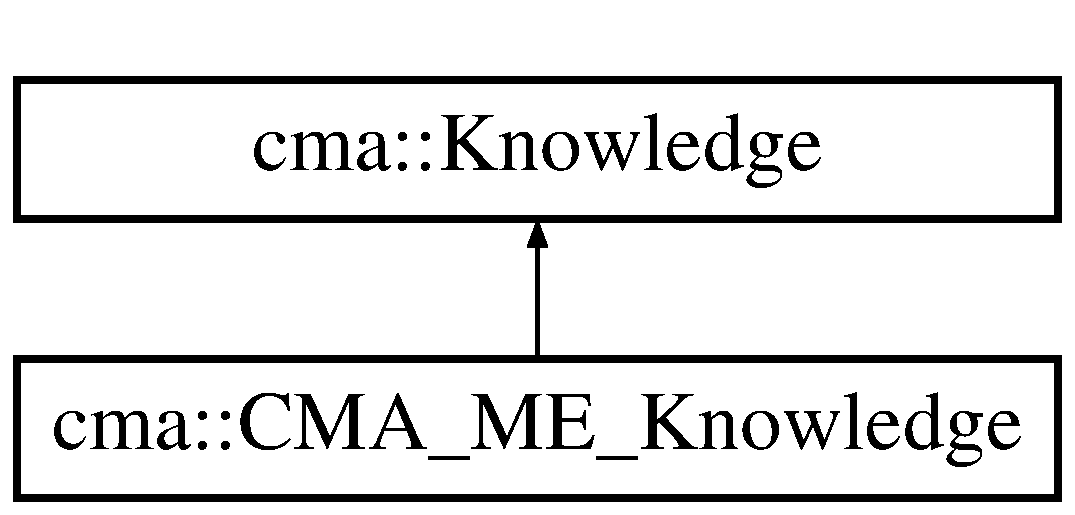
\includegraphics[height=2cm]{classcma_1_1Knowledge}
\end{center}
\end{figure}
\subsection*{Public Types}
\begin{CompactItemize}
\item 
enum {\bf EncodeType} \{ {\bf ENCODE\_\-TYPE\_\-GB2312}, 
{\bf ENCODE\_\-TYPE\_\-BIG5}, 
{\bf ENCODE\_\-TYPE\_\-UTF8}, 
{\bf ENCODE\_\-TYPE\_\-NUM}
 \}
\end{CompactItemize}
\subsection*{Public Member Functions}
\begin{CompactItemize}
\item 
virtual int {\bf loadSystemDict} (const char $\ast$binFileName)=0
\item 
virtual int {\bf loadUserDict} (const char $\ast$fileName)=0
\item 
virtual int {\bf loadStopWordDict} (const char $\ast$fileName)=0
\item 
virtual int {\bf loadStatModel} (const char $\ast$binFileName)=0
\item 
virtual int {\bf loadPOSModel} (const char $\ast$binFileName)=0
\item 
virtual int {\bf loadConfig} (const char $\ast$fileName)=0
\item 
virtual int {\bf encodeSystemDict} (const char $\ast$txtFileName, const char $\ast$binFileName)=0
\item 
void {\bf setEncodeType} ({\bf EncodeType} type)
\item 
{\bf EncodeType} {\bf getEncodeType} () const 
\end{CompactItemize}


\subsection{Detailed Description}
\doxyref{Knowledge}{p.}{classcma_1_1Knowledge} manages the linguistic information for Chinese morphological analysis. 

\subsection{Member Enumeration Documentation}
\index{cma::Knowledge@{cma::Knowledge}!EncodeType@{EncodeType}}
\index{EncodeType@{EncodeType}!cma::Knowledge@{cma::Knowledge}}
\subsubsection{\setlength{\rightskip}{0pt plus 5cm}enum {\bf cma::Knowledge::EncodeType}}\label{classcma_1_1Knowledge_2f725921dec755cdd496e81a95389f1d}


Encode type of characters. \begin{Desc}
\item[Enumerator: ]\par
\begin{description}
\index{ENCODE\_\-TYPE\_\-GB2312@{ENCODE\_\-TYPE\_\-GB2312}!cma::Knowledge@{cma::Knowledge}}\index{cma::Knowledge@{cma::Knowledge}!ENCODE\_\-TYPE\_\-GB2312@{ENCODE\_\-TYPE\_\-GB2312}}\item[{\em 
ENCODE\_\-TYPE\_\-GB2312\label{classcma_1_1Knowledge_2f725921dec755cdd496e81a95389f1d763b86f1378cda2ae30f3690a8c67b0d}
}]GB 2312 character type. \index{ENCODE\_\-TYPE\_\-BIG5@{ENCODE\_\-TYPE\_\-BIG5}!cma::Knowledge@{cma::Knowledge}}\index{cma::Knowledge@{cma::Knowledge}!ENCODE\_\-TYPE\_\-BIG5@{ENCODE\_\-TYPE\_\-BIG5}}\item[{\em 
ENCODE\_\-TYPE\_\-BIG5\label{classcma_1_1Knowledge_2f725921dec755cdd496e81a95389f1dfd187e4741157876b1a805c0c3ddec27}
}]Big 5 character type. \index{ENCODE\_\-TYPE\_\-UTF8@{ENCODE\_\-TYPE\_\-UTF8}!cma::Knowledge@{cma::Knowledge}}\index{cma::Knowledge@{cma::Knowledge}!ENCODE\_\-TYPE\_\-UTF8@{ENCODE\_\-TYPE\_\-UTF8}}\item[{\em 
ENCODE\_\-TYPE\_\-UTF8\label{classcma_1_1Knowledge_2f725921dec755cdd496e81a95389f1dc1a4019681243fa73708e4879f3b951d}
}]UTF8 character type. \index{ENCODE\_\-TYPE\_\-NUM@{ENCODE\_\-TYPE\_\-NUM}!cma::Knowledge@{cma::Knowledge}}\index{cma::Knowledge@{cma::Knowledge}!ENCODE\_\-TYPE\_\-NUM@{ENCODE\_\-TYPE\_\-NUM}}\item[{\em 
ENCODE\_\-TYPE\_\-NUM\label{classcma_1_1Knowledge_2f725921dec755cdd496e81a95389f1dfeaa8f94b6c57c430302ea94c41b1d8a}
}]the count of character types \end{description}
\end{Desc}



\subsection{Member Function Documentation}
\index{cma::Knowledge@{cma::Knowledge}!loadSystemDict@{loadSystemDict}}
\index{loadSystemDict@{loadSystemDict}!cma::Knowledge@{cma::Knowledge}}
\subsubsection{\setlength{\rightskip}{0pt plus 5cm}virtual int cma::Knowledge::loadSystemDict (const char $\ast$ {\em binFileName})\hspace{0.3cm}{\tt  [pure virtual]}}\label{classcma_1_1Knowledge_920159ccb5752992ea7ac7e87eedd1c0}


Load the system dictionary file, which is in binary format. \begin{Desc}
\item[Parameters:]
\begin{description}
\item[{\em binFileName}]the file name \end{description}
\end{Desc}
\begin{Desc}
\item[Returns:]0 for fail, 1 for success \end{Desc}


Implemented in {\bf cma::CMA\_\-ME\_\-Knowledge} \doxyref{}{p.}{classcma_1_1CMA__ME__Knowledge_247a1219355019e39e7caecfb84a8636}.\index{cma::Knowledge@{cma::Knowledge}!loadUserDict@{loadUserDict}}
\index{loadUserDict@{loadUserDict}!cma::Knowledge@{cma::Knowledge}}
\subsubsection{\setlength{\rightskip}{0pt plus 5cm}virtual int cma::Knowledge::loadUserDict (const char $\ast$ {\em fileName})\hspace{0.3cm}{\tt  [pure virtual]}}\label{classcma_1_1Knowledge_739fb78f864bef65fbb70b728492311f}


Load the user dictionary file, which is in text format. \begin{Desc}
\item[Parameters:]
\begin{description}
\item[{\em fileName}]the file name \end{description}
\end{Desc}
\begin{Desc}
\item[Returns:]0 for fail, 1 for success \end{Desc}


Implemented in {\bf cma::CMA\_\-ME\_\-Knowledge} \doxyref{}{p.}{classcma_1_1CMA__ME__Knowledge_d0dac8d22ab4c3c97a281f26c95ee9e2}.

Referenced by beginSeg().\index{cma::Knowledge@{cma::Knowledge}!loadStopWordDict@{loadStopWordDict}}
\index{loadStopWordDict@{loadStopWordDict}!cma::Knowledge@{cma::Knowledge}}
\subsubsection{\setlength{\rightskip}{0pt plus 5cm}virtual int cma::Knowledge::loadStopWordDict (const char $\ast$ {\em fileName})\hspace{0.3cm}{\tt  [pure virtual]}}\label{classcma_1_1Knowledge_992bf7b7cd77c8846bc1c6cd22067d07}


Load the stop-word dictionary file, which is in text format. The words in this file are ignored in the morphological analysis result. \begin{Desc}
\item[Parameters:]
\begin{description}
\item[{\em fileName}]the file name \end{description}
\end{Desc}
\begin{Desc}
\item[Returns:]0 for fail, 1 for success \end{Desc}


Implemented in {\bf cma::CMA\_\-ME\_\-Knowledge} \doxyref{}{p.}{classcma_1_1CMA__ME__Knowledge_ef7750521cda2746bae8325f37dc9a48}.\index{cma::Knowledge@{cma::Knowledge}!loadStatModel@{loadStatModel}}
\index{loadStatModel@{loadStatModel}!cma::Knowledge@{cma::Knowledge}}
\subsubsection{\setlength{\rightskip}{0pt plus 5cm}virtual int cma::Knowledge::loadStatModel (const char $\ast$ {\em binFileName})\hspace{0.3cm}{\tt  [pure virtual]}}\label{classcma_1_1Knowledge_c54810dbc59c5c5df69c7bef38fb0d51}


Load the model file in binary format, which contains statistical information for word segmentation. \begin{Desc}
\item[Parameters:]
\begin{description}
\item[{\em binFileName}]the file name \end{description}
\end{Desc}
\begin{Desc}
\item[Returns:]0 for fail, 1 for success \end{Desc}


Implemented in {\bf cma::CMA\_\-ME\_\-Knowledge} \doxyref{}{p.}{classcma_1_1CMA__ME__Knowledge_cc8f15814d4e6a248f29636a29116756}.

Referenced by beginSeg().\index{cma::Knowledge@{cma::Knowledge}!loadPOSModel@{loadPOSModel}}
\index{loadPOSModel@{loadPOSModel}!cma::Knowledge@{cma::Knowledge}}
\subsubsection{\setlength{\rightskip}{0pt plus 5cm}virtual int cma::Knowledge::loadPOSModel (const char $\ast$ {\em binFileName})\hspace{0.3cm}{\tt  [pure virtual]}}\label{classcma_1_1Knowledge_4ceb02d9154efd5bd8e35dfab9777644}


Load the model file in binary format, which contains statistical information for part-of-speech tagging. \begin{Desc}
\item[Parameters:]
\begin{description}
\item[{\em binFileName}]the file name \end{description}
\end{Desc}
\begin{Desc}
\item[Returns:]0 for fail, 1 for success \end{Desc}


Implemented in {\bf cma::CMA\_\-ME\_\-Knowledge} \doxyref{}{p.}{classcma_1_1CMA__ME__Knowledge_29a87c6902ebaf8364fbee0e4aa20127}.

Referenced by beginSeg().\index{cma::Knowledge@{cma::Knowledge}!loadConfig@{loadConfig}}
\index{loadConfig@{loadConfig}!cma::Knowledge@{cma::Knowledge}}
\subsubsection{\setlength{\rightskip}{0pt plus 5cm}virtual int cma::Knowledge::loadConfig (const char $\ast$ {\em fileName})\hspace{0.3cm}{\tt  [pure virtual]}}\label{classcma_1_1Knowledge_e4e24baf6f35004fd1d788b1b28a7ad1}


Load the configuration file, which is in text format. This file contains the configuration used in morphological analysis, such as part-of-speech configuration, etc. \begin{Desc}
\item[Parameters:]
\begin{description}
\item[{\em fileName}]the file name \end{description}
\end{Desc}
\begin{Desc}
\item[Returns:]0 for fail, 1 for success \end{Desc}


Implemented in {\bf cma::CMA\_\-ME\_\-Knowledge} \doxyref{}{p.}{classcma_1_1CMA__ME__Knowledge_74836fae9065f4c4869a2dde144a5f63}.\index{cma::Knowledge@{cma::Knowledge}!encodeSystemDict@{encodeSystemDict}}
\index{encodeSystemDict@{encodeSystemDict}!cma::Knowledge@{cma::Knowledge}}
\subsubsection{\setlength{\rightskip}{0pt plus 5cm}virtual int cma::Knowledge::encodeSystemDict (const char $\ast$ {\em txtFileName}, \/  const char $\ast$ {\em binFileName})\hspace{0.3cm}{\tt  [pure virtual]}}\label{classcma_1_1Knowledge_7c89dffabc4e75961d760586db283d1d}


Encode the system dictionary file from text to binary format. \begin{Desc}
\item[Parameters:]
\begin{description}
\item[{\em txtFileName}]the text file name \item[{\em binFileName}]the binary file name \end{description}
\end{Desc}
\begin{Desc}
\item[Returns:]0 for fail, 1 for success \end{Desc}


Implemented in {\bf cma::CMA\_\-ME\_\-Knowledge} \doxyref{}{p.}{classcma_1_1CMA__ME__Knowledge_578eab67c328dcde77c359f54cb6557f}.\index{cma::Knowledge@{cma::Knowledge}!setEncodeType@{setEncodeType}}
\index{setEncodeType@{setEncodeType}!cma::Knowledge@{cma::Knowledge}}
\subsubsection{\setlength{\rightskip}{0pt plus 5cm}void cma::Knowledge::setEncodeType ({\bf EncodeType} {\em type})}\label{classcma_1_1Knowledge_199293f2ec784e7883805117e59b109c}


Set the character encode type. If this function is not called, the default value returned by {\em \doxyref{getEncodeType()}{p.}{classcma_1_1Knowledge_26dac4378bb4192a598118abdef70ad9}\/} is {\em ENCODE\_\-TYPE\_\-GB2312\/}. \begin{Desc}
\item[Parameters:]
\begin{description}
\item[{\em type}]the encode type \end{description}
\end{Desc}


Referenced by beginSeg().\index{cma::Knowledge@{cma::Knowledge}!getEncodeType@{getEncodeType}}
\index{getEncodeType@{getEncodeType}!cma::Knowledge@{cma::Knowledge}}
\subsubsection{\setlength{\rightskip}{0pt plus 5cm}{\bf Knowledge::EncodeType} cma::Knowledge::getEncodeType () const}\label{classcma_1_1Knowledge_26dac4378bb4192a598118abdef70ad9}


Get the character encode type. \begin{Desc}
\item[Returns:]the encode type \end{Desc}


Referenced by cma::CMA\_\-ME\_\-Analyzer::setKnowledge().

The documentation for this class was generated from the following files:\begin{CompactItemize}
\item 
include/{\bf knowledge.h}\item 
source/src/{\bf knowledge.cpp}\end{CompactItemize}

\section{cma::Morpheme Struct Reference}
\label{structcma_1_1Morpheme}\index{cma::Morpheme@{cma::Morpheme}}
a pair of lexicon string and its part-of-speech tag.  


{\tt \#include $<$sentence.h$>$}

\subsection*{Public Member Functions}
\begin{CompactItemize}
\item 
{\bf Morpheme} ()
\end{CompactItemize}
\subsection*{Public Attributes}
\begin{CompactItemize}
\item 
std::string {\bf lexicon\_\-}
\item 
int {\bf posCode\_\-}
\end{CompactItemize}


\subsection{Detailed Description}
a pair of lexicon string and its part-of-speech tag. 

\doxyref{Morpheme}{p.}{structcma_1_1Morpheme} is a pair of lexicon string and its part-of-speech tag. 

\subsection{Constructor \& Destructor Documentation}
\index{cma::Morpheme@{cma::Morpheme}!Morpheme@{Morpheme}}
\index{Morpheme@{Morpheme}!cma::Morpheme@{cma::Morpheme}}
\subsubsection{\setlength{\rightskip}{0pt plus 5cm}cma::Morpheme::Morpheme ()}\label{structcma_1_1Morpheme_79ab5404cd959f89daadb8a7714334cb}


Constructor. The lexicon string value is initialized with empty string, and the index code of part-of-speech tag is initialized with -1, meaning that no part-of-speech tag is available. 

\subsection{Member Data Documentation}
\index{cma::Morpheme@{cma::Morpheme}!lexicon\_\-@{lexicon\_\-}}
\index{lexicon\_\-@{lexicon\_\-}!cma::Morpheme@{cma::Morpheme}}
\subsubsection{\setlength{\rightskip}{0pt plus 5cm}std::string {\bf cma::Morpheme::lexicon\_\-}}\label{structcma_1_1Morpheme_1054ad519e1ebb80ec71cd21b8ad2a78}


the lexicon string value 

Referenced by cma::CMA\_\-ME\_\-Analyzer::runWithSentence().\index{cma::Morpheme@{cma::Morpheme}!posCode\_\-@{posCode\_\-}}
\index{posCode\_\-@{posCode\_\-}!cma::Morpheme@{cma::Morpheme}}
\subsubsection{\setlength{\rightskip}{0pt plus 5cm}int {\bf cma::Morpheme::posCode\_\-}}\label{structcma_1_1Morpheme_883d0df2e303ce7bd5953bfa913a88ef}


the index code of part-of-speech tag 

Referenced by cma::CMA\_\-ME\_\-Analyzer::runWithSentence().

The documentation for this struct was generated from the following files:\begin{CompactItemize}
\item 
include/{\bf sentence.h}\item 
source/src/{\bf sentence.cpp}\end{CompactItemize}

\section{cma::Nocase Class Reference}
\label{classcma_1_1Nocase}\index{cma::Nocase@{cma::Nocase}}
Case-insensitive string compare.  


{\tt \#include $<$pos\_\-table.h$>$}

\subsection*{Public Member Functions}
\begin{CompactItemize}
\item 
bool {\bf operator()} (const std::string \&x, const std::string \&y) const 
\end{CompactItemize}


\subsection{Detailed Description}
Case-insensitive string compare. 

Case-insensitive string compare. 

\subsection{Member Function Documentation}
\index{cma::Nocase@{cma::Nocase}!operator()@{operator()}}
\index{operator()@{operator()}!cma::Nocase@{cma::Nocase}}
\subsubsection{\setlength{\rightskip}{0pt plus 5cm}bool cma::Nocase::operator() (const std::string \& {\em x}, \/  const std::string \& {\em y}) const}\label{classcma_1_1Nocase_26ede1cd9f2d4ee5796af335019014e1}


Compare string case-insensitively. \begin{Desc}
\item[Parameters:]
\begin{description}
\item[{\em x}]the first string \item[{\em y}]the second string \end{description}
\end{Desc}
\begin{Desc}
\item[Returns:]true if {\em x\/} is lexicographically less than {\em y\/}, not taking case into account \end{Desc}


The documentation for this class was generated from the following files:\begin{CompactItemize}
\item 
source/include/{\bf pos\_\-table.h}\item 
source/src/{\bf pos\_\-table.cpp}\end{CompactItemize}

\section{cma::POSTable Class Reference}
\label{classcma_1_1POSTable}\index{cma::POSTable@{cma::POSTable}}
\doxyref{POSTable}{p.}{classcma_1_1POSTable} stores the global table of part-of-speech tags.  


{\tt \#include $<$pos\_\-table.h$>$}

\subsection*{Public Member Functions}
\begin{CompactItemize}
\item 
int {\bf addPOS} (const std::string \&pos)
\item 
int {\bf getCodeFromStr} (const std::string \&pos) const 
\item 
const char $\ast$ {\bf getStrFromCode} (int index) const 
\item 
int {\bf size} () const 
\end{CompactItemize}
\subsection*{Static Public Member Functions}
\begin{CompactItemize}
\item 
static {\bf POSTable} $\ast$ {\bf instance} ()
\end{CompactItemize}


\subsection{Detailed Description}
\doxyref{POSTable}{p.}{classcma_1_1POSTable} stores the global table of part-of-speech tags. 

\doxyref{POSTable}{p.}{classcma_1_1POSTable} stores the global table of part-of-speech tags, each tag includes a string value and its index code. Note that the string value of part-of-speech tag is case-insensitive. For example, 'Ng' equals to 'ng'. 

\subsection{Member Function Documentation}
\index{cma::POSTable@{cma::POSTable}!instance@{instance}}
\index{instance@{instance}!cma::POSTable@{cma::POSTable}}
\subsubsection{\setlength{\rightskip}{0pt plus 5cm}{\bf POSTable} $\ast$ cma::POSTable::instance ()\hspace{0.3cm}{\tt  [static]}}\label{classcma_1_1POSTable_8ce731b2b76aced0b76092b5b216aa1d}


Create an instance of {\em \doxyref{POSTable}{p.}{classcma_1_1POSTable}\/}. \begin{Desc}
\item[Returns:]the pointer to instance \end{Desc}


Referenced by cma::Sentence::getStrPOS(), cma::CMA\_\-ME\_\-Knowledge::loadPOSModel(), and cma::CMA\_\-ME\_\-Analyzer::runWithSentence().\index{cma::POSTable@{cma::POSTable}!addPOS@{addPOS}}
\index{addPOS@{addPOS}!cma::POSTable@{cma::POSTable}}
\subsubsection{\setlength{\rightskip}{0pt plus 5cm}int cma::POSTable::addPOS (const std::string \& {\em pos})}\label{classcma_1_1POSTable_77898a33965a0eee826c41b7916d80ce}


Add the POS string to the global part-of-speech table. \begin{Desc}
\item[Parameters:]
\begin{description}
\item[{\em pos}]the POS string \end{description}
\end{Desc}
\begin{Desc}
\item[Returns:]the index code of the POS string added, if the POS string has been added before, its index code previously added is returned. \end{Desc}
\begin{Desc}
\item[Attention:]Note that the POS string is case-insensitively. \end{Desc}


Referenced by cma::CMA\_\-ME\_\-Knowledge::loadPOSModel().\index{cma::POSTable@{cma::POSTable}!getCodeFromStr@{getCodeFromStr}}
\index{getCodeFromStr@{getCodeFromStr}!cma::POSTable@{cma::POSTable}}
\subsubsection{\setlength{\rightskip}{0pt plus 5cm}int cma::POSTable::getCodeFromStr (const std::string \& {\em pos}) const}\label{classcma_1_1POSTable_1692f43e2154d408265e09affd64d70a}


Get the POS index code from the POS string in the global part-of-speech table. \begin{Desc}
\item[Parameters:]
\begin{description}
\item[{\em pos}]the POS string \end{description}
\end{Desc}
\begin{Desc}
\item[Returns:]POS index code, -1 for non POS available \end{Desc}


Referenced by cma::CMA\_\-ME\_\-Analyzer::runWithSentence().\index{cma::POSTable@{cma::POSTable}!getStrFromCode@{getStrFromCode}}
\index{getStrFromCode@{getStrFromCode}!cma::POSTable@{cma::POSTable}}
\subsubsection{\setlength{\rightskip}{0pt plus 5cm}const char $\ast$ cma::POSTable::getStrFromCode (int {\em index}) const}\label{classcma_1_1POSTable_cf9611088b3484dbaad11ef2b5b24f52}


Get the POS string from the POS index code in the global part-of-speech table. \begin{Desc}
\item[Parameters:]
\begin{description}
\item[{\em index}]the POS index code \end{description}
\end{Desc}
\begin{Desc}
\item[Returns:]POS string, null pointer for non POS available \end{Desc}


Referenced by cma::Sentence::getStrPOS().\index{cma::POSTable@{cma::POSTable}!size@{size}}
\index{size@{size}!cma::POSTable@{cma::POSTable}}
\subsubsection{\setlength{\rightskip}{0pt plus 5cm}int cma::POSTable::size () const}\label{classcma_1_1POSTable_eb70793af427c7dd545f132e177ca26e}


Get the number of POS tags in the global part-of-speech table. \begin{Desc}
\item[Returns:]the number of POS tags \end{Desc}


The documentation for this class was generated from the following files:\begin{CompactItemize}
\item 
source/include/{\bf pos\_\-table.h}\item 
source/src/{\bf pos\_\-table.cpp}\end{CompactItemize}

\section{cma::POSTagger Class Reference}
\label{classcma_1_1POSTagger}\index{cma::POSTagger@{cma::POSTagger}}
Tagging the POS Information Tagging the POS using the maxent model.  


{\tt \#include $<$CMAPOSTagger.h$>$}

\subsection*{Public Member Functions}
\begin{CompactItemize}
\item 
{\bf POSTagger} (const string \&model, {\bf VTrie} $\ast$pTrie)
\item 
{\bf POSTagger} (const string \&model, const char $\ast$dictFile)
\item 
void {\bf tag\_\-file} (const char $\ast$inFile, const char $\ast$outFile)
\item 
void {\bf tag\_\-sentence} (vector$<$ string $>$ \&words, size\_\-t N, size\_\-t retSize, vector$<$ pair$<$ vector$<$ string $>$, double $>$ $>$ \&segment)
\item 
void {\bf tag\_\-sentence\_\-best} (vector$<$ string $>$ \&words, vector$<$ string $>$ \&posRet, int begin, int end)
\item 
double {\bf tag\_\-word\_\-best} (vector$<$ string $>$ \&words, vector$<$ string $>$ \&poses, int index, string \&pos)
\item 
bool {\bf appendWordPOS} (string \&line)
\item 
void {\bf setCType} ({\bf CMA\_\-CType} $\ast$ctype)
\end{CompactItemize}


\subsection{Detailed Description}
Tagging the POS Information Tagging the POS using the maxent model. 

\subsection{Constructor \& Destructor Documentation}
\index{cma::POSTagger@{cma::POSTagger}!POSTagger@{POSTagger}}
\index{POSTagger@{POSTagger}!cma::POSTagger@{cma::POSTagger}}
\subsubsection{\setlength{\rightskip}{0pt plus 5cm}cma::POSTagger::POSTagger (const string \& {\em model}, \/  {\bf VTrie} $\ast$ {\em pTrie})}\label{classcma_1_1POSTagger_dd40a3098429d2febe81df1d943cc486}


Construct the \doxyref{POSTagger}{p.}{classcma_1_1POSTagger} with outer \doxyref{VTrie}{p.}{classVTrie} \begin{Desc}
\item[Parameters:]
\begin{description}
\item[{\em model}]POS model name \end{description}
\end{Desc}
\index{cma::POSTagger@{cma::POSTagger}!POSTagger@{POSTagger}}
\index{POSTagger@{POSTagger}!cma::POSTagger@{cma::POSTagger}}
\subsubsection{\setlength{\rightskip}{0pt plus 5cm}cma::POSTagger::POSTagger (const string \& {\em model}, \/  const char $\ast$ {\em dictFile})}\label{classcma_1_1POSTagger_678c73558ec8fb6f3ae1adc5a4d904bb}


Construct the \doxyref{POSTagger}{p.}{classcma_1_1POSTagger} with inner \doxyref{VTrie}{p.}{classVTrie} (read from dictFile) 

References appendWordPOS().

\subsection{Member Function Documentation}
\index{cma::POSTagger@{cma::POSTagger}!tag\_\-file@{tag\_\-file}}
\index{tag\_\-file@{tag\_\-file}!cma::POSTagger@{cma::POSTagger}}
\subsubsection{\setlength{\rightskip}{0pt plus 5cm}void cma::POSTagger::tag\_\-file (const char $\ast$ {\em inFile}, \/  const char $\ast$ {\em outFile})}\label{classcma_1_1POSTagger_95aa58e81425e379ef7100c5311a003b}


Tag the segmented file with pos (In UTF8 Encoding) \begin{Desc}
\item[Parameters:]
\begin{description}
\item[{\em inFile}]the input file \item[{\em outFile}]the output file \end{description}
\end{Desc}


References tag\_\-sentence\_\-best().\index{cma::POSTagger@{cma::POSTagger}!tag\_\-sentence@{tag\_\-sentence}}
\index{tag\_\-sentence@{tag\_\-sentence}!cma::POSTagger@{cma::POSTagger}}
\subsubsection{\setlength{\rightskip}{0pt plus 5cm}void cma::POSTagger::tag\_\-sentence (vector$<$ string $>$ \& {\em words}, \/  size\_\-t {\em N}, \/  size\_\-t {\em retSize}, \/  vector$<$ pair$<$ vector$<$ string $>$, double $>$ $>$ \& {\em segment})}\label{classcma_1_1POSTagger_17818fb91478d21edcaa741c9d43d295}


tagging given words list and return N best \begin{Desc}
\item[Parameters:]
\begin{description}
\item[{\em words}]the given words list \item[{\em N}]return N best \item[{\em retSize}]retSize $<$= N, the size of segment \item[{\em to}]store the result value \end{description}
\end{Desc}


References cma::POSTagUnit::index, cma::POSTagUnit::pos, cma::POSTagUnit::previous, and cma::POSTagUnit::score.\index{cma::POSTagger@{cma::POSTagger}!tag\_\-sentence\_\-best@{tag\_\-sentence\_\-best}}
\index{tag\_\-sentence\_\-best@{tag\_\-sentence\_\-best}!cma::POSTagger@{cma::POSTagger}}
\subsubsection{\setlength{\rightskip}{0pt plus 5cm}void cma::POSTagger::tag\_\-sentence\_\-best (vector$<$ string $>$ \& {\em words}, \/  vector$<$ string $>$ \& {\em posRet}, \/  int {\em begin}, \/  int {\em end})}\label{classcma_1_1POSTagger_efb7b6cfd52c11d289fb8f2332dde7c4}


Only return the best result \begin{Desc}
\item[Parameters:]
\begin{description}
\item[{\em words}]words vector \item[{\em posRet}]to hold the result value \item[{\em begin}]the begin index (include) to check \item[{\em end}]the first index that should not check \end{description}
\end{Desc}


Referenced by tag\_\-file().\index{cma::POSTagger@{cma::POSTagger}!tag\_\-word\_\-best@{tag\_\-word\_\-best}}
\index{tag\_\-word\_\-best@{tag\_\-word\_\-best}!cma::POSTagger@{cma::POSTagger}}
\subsubsection{\setlength{\rightskip}{0pt plus 5cm}double cma::POSTagger::tag\_\-word\_\-best (vector$<$ string $>$ \& {\em words}, \/  vector$<$ string $>$ \& {\em poses}, \/  int {\em index}, \/  string \& {\em pos})}\label{classcma_1_1POSTagger_c7d4c9b62c95e138f39dc84624f11b2e}


tag the word with the best POS and return its score \begin{Desc}
\item[Parameters:]
\begin{description}
\item[{\em words}]words vector \item[{\em poses}]the previous pos vector, but the current pos won't store into the poses \item[{\em index}]the current index to check \item[{\em pos}]to store the best pos \end{description}
\end{Desc}
\begin{Desc}
\item[Returns:]return the score of the best pos \end{Desc}
\index{cma::POSTagger@{cma::POSTagger}!appendWordPOS@{appendWordPOS}}
\index{appendWordPOS@{appendWordPOS}!cma::POSTagger@{cma::POSTagger}}
\subsubsection{\setlength{\rightskip}{0pt plus 5cm}bool cma::POSTagger::appendWordPOS (string \& {\em line})}\label{classcma_1_1POSTagger_e3a219f6213b4ec917255af7f508f343}


Append the POS Information into Trie and POS Vector \begin{Desc}
\item[Parameters:]
\begin{description}
\item[{\em line}]a line like: word1 pos1 pos2 ... posN \end{description}
\end{Desc}
\begin{Desc}
\item[Returns:]whether add successfully \end{Desc}


References VTrieNode::data, VTrie::insert(), and VTrie::search().

Referenced by cma::CMA\_\-ME\_\-Knowledge::loadSystemDict(), cma::CMA\_\-ME\_\-Knowledge::loadUserDict(), and POSTagger().\index{cma::POSTagger@{cma::POSTagger}!setCType@{setCType}}
\index{setCType@{setCType}!cma::POSTagger@{cma::POSTagger}}
\subsubsection{\setlength{\rightskip}{0pt plus 5cm}void cma::POSTagger::setCType ({\bf CMA\_\-CType} $\ast$ {\em ctype})\hspace{0.3cm}{\tt  [inline]}}\label{classcma_1_1POSTagger_cf191ab0490ea004e681c93c901de355}


Set the reference to the specific character encoding

\begin{Desc}
\item[Parameters:]
\begin{description}
\item[{\em ctype}]new specific character encoding \end{description}
\end{Desc}


Referenced by cma::CMA\_\-ME\_\-Analyzer::setKnowledge().

The documentation for this class was generated from the following files:\begin{CompactItemize}
\item 
source/include/CMAPOSTagger.h\item 
source/src/CMAPOSTagger.cc\end{CompactItemize}

\section{cma::SegTagger Class Reference}
\label{classcma_1_1SegTagger}\index{cma::SegTagger@{cma::SegTagger}}
segment the string segment the string using maxent model  


{\tt \#include $<$CMAPOCTagger.h$>$}

\subsection*{Public Member Functions}
\begin{CompactItemize}
\item 
{\bf SegTagger} (const string \&cateName, {\bf VTrie} $\ast$posTrie, double eScore=0.7)
\item 
void \textbf{tag\_\-file} (const char $\ast$inFile, const char $\ast$outFile, string encType=\char`\"{}gb2312\char`\"{})\label{classcma_1_1SegTagger_a25c24f24bbd54dac4e77cef92cf1e11}

\item 
void {\bf seg\_\-sentence} (vector$<$ string $>$ \&words, CharType $\ast$types, size\_\-t N, size\_\-t retSize, vector$<$ pair$<$ vector$<$ string $>$, double $>$ $>$ \&segment)
\item 
void {\bf seg\_\-sentence\_\-best} (vector$<$ string $>$ \&words, CharType $\ast$types, vector$<$ string $>$ \&segment)
\item 
void \textbf{setCType} ({\bf CMA\_\-CType} $\ast$ctype)\label{classcma_1_1SegTagger_a2c314b48a8fdb5ddc09df9a244dae91}

\item 
void {\bf setEScore} (double eScore)
\item 
double {\bf getEScore} ()
\end{CompactItemize}
\subsection*{Static Public Member Functions}
\begin{CompactItemize}
\item 
static void {\bf initialize} ()
\end{CompactItemize}


\subsection{Detailed Description}
segment the string segment the string using maxent model 

\subsection{Constructor \& Destructor Documentation}
\index{cma::SegTagger@{cma::SegTagger}!SegTagger@{SegTagger}}
\index{SegTagger@{SegTagger}!cma::SegTagger@{cma::SegTagger}}
\subsubsection{\setlength{\rightskip}{0pt plus 5cm}cma::SegTagger::SegTagger (const string \& {\em cateName}, \/  {\bf VTrie} $\ast$ {\em posTrie}, \/  double {\em eScore} = {\tt 0.7})}\label{classcma_1_1SegTagger_f43fe12512609241653aeb28d02a3811}


Create the \doxyref{SegTagger}{p.}{classcma_1_1SegTagger} \begin{Desc}
\item[Parameters:]
\begin{description}
\item[{\em cateName}]the poc category name, the model file(cateName + \char`\"{}.model\char`\"{}) should exists. \item[{\em posTrie}]the \doxyref{VTrie}{p.}{classVTrie} to hold the POS Information \item[{\em eScore}]is a double value between 0.5 and 1.0, if the POC tag B has possiblity more the eScore, it will be tagged with E. EScore's default value is 0.7. \end{description}
\end{Desc}


References initialize(), and setEScore().

\subsection{Member Function Documentation}
\index{cma::SegTagger@{cma::SegTagger}!seg\_\-sentence@{seg\_\-sentence}}
\index{seg\_\-sentence@{seg\_\-sentence}!cma::SegTagger@{cma::SegTagger}}
\subsubsection{\setlength{\rightskip}{0pt plus 5cm}void cma::SegTagger::seg\_\-sentence (vector$<$ string $>$ \& {\em words}, \/  CharType $\ast$ {\em types}, \/  size\_\-t {\em N}, \/  size\_\-t {\em retSize}, \/  vector$<$ pair$<$ vector$<$ string $>$, double $>$ $>$ \& {\em segment})}\label{classcma_1_1SegTagger_1bc4a830d793b5e0bb142ea5061fff09}


tagging given words list and return N best \begin{Desc}
\item[Parameters:]
\begin{description}
\item[{\em words}]the given words list \item[{\em N}]return N best \item[{\em retSize}]retSize $<$= N, the size of segment \end{description}
\end{Desc}
\index{cma::SegTagger@{cma::SegTagger}!seg\_\-sentence\_\-best@{seg\_\-sentence\_\-best}}
\index{seg\_\-sentence\_\-best@{seg\_\-sentence\_\-best}!cma::SegTagger@{cma::SegTagger}}
\subsubsection{\setlength{\rightskip}{0pt plus 5cm}void cma::SegTagger::seg\_\-sentence\_\-best (vector$<$ string $>$ \& {\em words}, \/  CharType $\ast$ {\em types}, \/  vector$<$ string $>$ \& {\em segment})}\label{classcma_1_1SegTagger_c2b95d3cfb82743cf5cc29f8e196a6e1}


only return the best segment result, no scores is used here \begin{Desc}
\item[Parameters:]
\begin{description}
\item[{\em words}]the word list \item[{\em segment}]to store the segmented words \end{description}
\end{Desc}


References cma::pocinner::StrBasedVTrie::completeSearch, cma::pocinner::StrBasedVTrie::firstSearch(), and cma::pocinner::StrBasedVTrie::search().\index{cma::SegTagger@{cma::SegTagger}!initialize@{initialize}}
\index{initialize@{initialize}!cma::SegTagger@{cma::SegTagger}}
\subsubsection{\setlength{\rightskip}{0pt plus 5cm}void cma::SegTagger::initialize ()\hspace{0.3cm}{\tt  [static]}}\label{classcma_1_1SegTagger_03888848517344bd7e221d61aa7954d4}


Would be invoked by the SegTagger's Constructor 

Referenced by SegTagger().\index{cma::SegTagger@{cma::SegTagger}!setEScore@{setEScore}}
\index{setEScore@{setEScore}!cma::SegTagger@{cma::SegTagger}}
\subsubsection{\setlength{\rightskip}{0pt plus 5cm}void cma::SegTagger::setEScore (double {\em eScore})\hspace{0.3cm}{\tt  [inline]}}\label{classcma_1_1SegTagger_695b30814b6c10cbdfb92434979a284c}


Set the EScore\par
 EScore is a double value between 0.5 and 1.0, if the POC tag B has possiblity more the eScore, it will be tagged with E. \par
 EScore's default value is 0.7.

\begin{Desc}
\item[Returns:]eScore the new eScore \end{Desc}


Referenced by SegTagger().\index{cma::SegTagger@{cma::SegTagger}!getEScore@{getEScore}}
\index{getEScore@{getEScore}!cma::SegTagger@{cma::SegTagger}}
\subsubsection{\setlength{\rightskip}{0pt plus 5cm}double cma::SegTagger::getEScore ()\hspace{0.3cm}{\tt  [inline]}}\label{classcma_1_1SegTagger_864f555f4a72d46a6f395b1e4bfe1459}


Get the EScore \par
 EScore is a double value between 0.5 and 1.0, if the POC tag B has possiblity more the eScore, it will be tagged with E. \par
 EScore's default value is 0.7.

\begin{Desc}
\item[Returns:]the EScore \end{Desc}


The documentation for this class was generated from the following files:\begin{CompactItemize}
\item 
source/include/CMAPOCTagger.h\item 
source/src/CMAPOCTagger.cc\end{CompactItemize}

\section{cma::Sentence Class Reference}
\label{classcma_1_1Sentence}\index{cma::Sentence@{cma::Sentence}}
\doxyref{Sentence}{p.}{classcma_1_1Sentence} saves the results of Chinese morphological analysis.  


{\tt \#include $<$sentence.h$>$}

\subsection*{Public Member Functions}
\begin{CompactItemize}
\item 
void {\bf setString} (const char $\ast$pString)
\item 
const char $\ast$ {\bf getString} (void) const 
\item 
int {\bf getListSize} (void) const 
\item 
int {\bf getCount} (int nPos) const 
\item 
const char $\ast$ {\bf getLexicon} (int nPos, int nIdx) const 
\item 
int {\bf getPOS} (int nPos, int nIdx) const 
\item 
const char $\ast$ {\bf getStrPOS} (int nPos, int nIdx) const 
\item 
double {\bf getScore} (int nPos) const 
\item 
int {\bf getOneBestIndex} (void) const 
\item 
void {\bf addList} (const MorphemeList \&morphemeList, double score=0.0)
\end{CompactItemize}


\subsection{Detailed Description}
\doxyref{Sentence}{p.}{classcma_1_1Sentence} saves the results of Chinese morphological analysis. 

\doxyref{Sentence}{p.}{classcma_1_1Sentence} saves the results of Chinese morphological analysis. Typically, the usage is like below:

\doxyref{Sentence}{p.}{classcma_1_1Sentence} s; s.setString(\char`\"{}...\char`\"{});

Analyzer$\ast$ analyzer = ...; analyzer-$>$runWithSentence(s);

// get n-best results for(int i=0; i$<$s.getListSize(); ++i) \{ for(int j=0; j$<$s.getCount(i); ++j) \{ const char$\ast$ pLexicon = s.getLexicon(i, j); const char$\ast$ strPOS = s.getStrPOS(i, j); ... \} double score = s.getScore(i); ... \}

// get one-best result int i= s.getOneBestIndex(); ... 

\subsection{Member Function Documentation}
\index{cma::Sentence@{cma::Sentence}!setString@{setString}}
\index{setString@{setString}!cma::Sentence@{cma::Sentence}}
\subsubsection{\setlength{\rightskip}{0pt plus 5cm}void cma::Sentence::setString (const char $\ast$ {\em pString})}\label{classcma_1_1Sentence_40fb665bd2b2a19e430d4e474f3534a3}


Set the raw sentence string. \begin{Desc}
\item[Parameters:]
\begin{description}
\item[{\em pString}]value of the raw string \end{description}
\end{Desc}
\begin{Desc}
\item[Attention:]the previous analysis results will be removed. \end{Desc}
\index{cma::Sentence@{cma::Sentence}!getString@{getString}}
\index{getString@{getString}!cma::Sentence@{cma::Sentence}}
\subsubsection{\setlength{\rightskip}{0pt plus 5cm}const char $\ast$ cma::Sentence::getString (void) const}\label{classcma_1_1Sentence_ee44e192f67dacbe6bc0cfc433cabb30}


Get the raw sentence string. \begin{Desc}
\item[Returns:]value of the raw string \end{Desc}


Referenced by cma::CMA\_\-ME\_\-Analyzer::runWithSentence().\index{cma::Sentence@{cma::Sentence}!getListSize@{getListSize}}
\index{getListSize@{getListSize}!cma::Sentence@{cma::Sentence}}
\subsubsection{\setlength{\rightskip}{0pt plus 5cm}int cma::Sentence::getListSize (void) const}\label{classcma_1_1Sentence_883c3773c3f2a82f3b3b9fcae13ceb66}


Get the number of candidates of morphological analysis result. \begin{Desc}
\item[Returns:]the number of candidates \end{Desc}
\index{cma::Sentence@{cma::Sentence}!getCount@{getCount}}
\index{getCount@{getCount}!cma::Sentence@{cma::Sentence}}
\subsubsection{\setlength{\rightskip}{0pt plus 5cm}int cma::Sentence::getCount (int {\em nPos}) const}\label{classcma_1_1Sentence_5dd92e59708ea8cc61d3edc0d1fd830d}


Get the number of morphemes in candidate result {\em nPos\/}. \begin{Desc}
\item[Parameters:]
\begin{description}
\item[{\em nPos}]candidate result index \end{description}
\end{Desc}
\begin{Desc}
\item[Returns:]the number of morphemes \end{Desc}
\index{cma::Sentence@{cma::Sentence}!getLexicon@{getLexicon}}
\index{getLexicon@{getLexicon}!cma::Sentence@{cma::Sentence}}
\subsubsection{\setlength{\rightskip}{0pt plus 5cm}const char $\ast$ cma::Sentence::getLexicon (int {\em nPos}, \/  int {\em nIdx}) const}\label{classcma_1_1Sentence_c8fd1b3aa8062fff6e88a31e723802ae}


Get the string of morpheme {\em nIdx\/} in candidate result {\em nPos\/}. \begin{Desc}
\item[Parameters:]
\begin{description}
\item[{\em nPos}]candidate result index \item[{\em nIdx}]morpheme index \end{description}
\end{Desc}
\begin{Desc}
\item[Returns:]morpheme string \end{Desc}
\index{cma::Sentence@{cma::Sentence}!getPOS@{getPOS}}
\index{getPOS@{getPOS}!cma::Sentence@{cma::Sentence}}
\subsubsection{\setlength{\rightskip}{0pt plus 5cm}int cma::Sentence::getPOS (int {\em nPos}, \/  int {\em nIdx}) const}\label{classcma_1_1Sentence_7e03360cc524ea35245c1b5a61c348e0}


Get the POS index code of morpheme {\em nIdx\/} in candidate result {\em nPos\/}. \begin{Desc}
\item[Parameters:]
\begin{description}
\item[{\em nPos}]candidate result index \item[{\em nIdx}]morpheme index \end{description}
\end{Desc}
\begin{Desc}
\item[Returns:]POS index code, -1 for non POS available \end{Desc}


Referenced by getStrPOS().\index{cma::Sentence@{cma::Sentence}!getStrPOS@{getStrPOS}}
\index{getStrPOS@{getStrPOS}!cma::Sentence@{cma::Sentence}}
\subsubsection{\setlength{\rightskip}{0pt plus 5cm}const char $\ast$ cma::Sentence::getStrPOS (int {\em nPos}, \/  int {\em nIdx}) const}\label{classcma_1_1Sentence_6cb05837a84acf7d30fadb5bca6314db}


Get the POS string of morpheme {\em nIdx\/} in candidate result {\em nPos\/}. \begin{Desc}
\item[Parameters:]
\begin{description}
\item[{\em nPos}]candidate result index \item[{\em nIdx}]morpheme index \end{description}
\end{Desc}
\begin{Desc}
\item[Returns:]POS string, null pointer for non POS available \end{Desc}


References getPOS(), cma::POSTable::getStrFromCode(), and cma::POSTable::instance().\index{cma::Sentence@{cma::Sentence}!getScore@{getScore}}
\index{getScore@{getScore}!cma::Sentence@{cma::Sentence}}
\subsubsection{\setlength{\rightskip}{0pt plus 5cm}double cma::Sentence::getScore (int {\em nPos}) const}\label{classcma_1_1Sentence_850f236efa3fa2b75b5b40cf35fbdd95}


Get the score of candidate result {\em nPos\/}. \begin{Desc}
\item[Parameters:]
\begin{description}
\item[{\em nPos}]candidate result index \end{description}
\end{Desc}
\begin{Desc}
\item[Returns:]the score value \end{Desc}
\index{cma::Sentence@{cma::Sentence}!getOneBestIndex@{getOneBestIndex}}
\index{getOneBestIndex@{getOneBestIndex}!cma::Sentence@{cma::Sentence}}
\subsubsection{\setlength{\rightskip}{0pt plus 5cm}int cma::Sentence::getOneBestIndex (void) const}\label{classcma_1_1Sentence_f1ccc0e78beb1f7b8bd22e0c10efa8d4}


Get the index of the candidate result, which has the highest score. \begin{Desc}
\item[Returns:]candidate result index, -1 is returned if there is no candidate result. \end{Desc}
\index{cma::Sentence@{cma::Sentence}!addList@{addList}}
\index{addList@{addList}!cma::Sentence@{cma::Sentence}}
\subsubsection{\setlength{\rightskip}{0pt plus 5cm}void cma::Sentence::addList (const MorphemeList \& {\em morphemeList}, \/  double {\em score} = {\tt 0.0})}\label{classcma_1_1Sentence_39f0e77ac6f3705ae6dc1b8e15118760}


Add a candidate result of morphological analysis. \begin{Desc}
\item[Parameters:]
\begin{description}
\item[{\em morphemeList}]the candidate result \item[{\em score}]the score value of the candidate \end{description}
\end{Desc}


Referenced by cma::CMA\_\-ME\_\-Analyzer::runWithSentence().

The documentation for this class was generated from the following files:\begin{CompactItemize}
\item 
include/{\bf sentence.h}\item 
source/src/{\bf sentence.cpp}\end{CompactItemize}

\section{cma::pocinner::StrBasedVTrie Class Reference}
\label{classcma_1_1pocinner_1_1StrBasedVTrie}\index{cma::pocinner::StrBasedVTrie@{cma::pocinner::StrBasedVTrie}}
The utility class to search the string one by one.  


\subsection*{Public Member Functions}
\begin{CompactItemize}
\item 
{\bf StrBasedVTrie} ({\bf VTrie} $\ast$pTrie)
\item 
void {\bf reset} ()
\item 
bool {\bf search} (const char $\ast$p)
\item 
bool {\bf firstSearch} (const char $\ast$p)
\end{CompactItemize}
\subsection*{Public Attributes}
\begin{CompactItemize}
\item 
{\bf VTrie} $\ast$ {\bf trie}
\item 
{\bf VTrieNode} {\bf node}
\item 
bool {\bf completeSearch}
\end{CompactItemize}


\subsection{Detailed Description}
The utility class to search the string one by one. 

The utility class to search the string one by one 

\subsection{Constructor \& Destructor Documentation}
\index{cma::pocinner::StrBasedVTrie@{cma::pocinner::StrBasedVTrie}!StrBasedVTrie@{StrBasedVTrie}}
\index{StrBasedVTrie@{StrBasedVTrie}!cma::pocinner::StrBasedVTrie@{cma::pocinner::StrBasedVTrie}}
\subsubsection[{StrBasedVTrie}]{\setlength{\rightskip}{0pt plus 5cm}cma::pocinner::StrBasedVTrie::StrBasedVTrie ({\bf VTrie} $\ast$ {\em pTrie})\hspace{0.3cm}{\tt  [inline]}}\label{classcma_1_1pocinner_1_1StrBasedVTrie_8fea04163cec0e1ca5c55f024549f2cd}


Create an instance

\begin{Desc}
\item[Parameters:]
\begin{description}
\item[{\em pTrie}]the \doxyref{VTrie}{p.}{classVTrie} \end{description}
\end{Desc}


\subsection{Member Function Documentation}
\index{cma::pocinner::StrBasedVTrie@{cma::pocinner::StrBasedVTrie}!firstSearch@{firstSearch}}
\index{firstSearch@{firstSearch}!cma::pocinner::StrBasedVTrie@{cma::pocinner::StrBasedVTrie}}
\subsubsection[{firstSearch}]{\setlength{\rightskip}{0pt plus 5cm}bool cma::pocinner::StrBasedVTrie::firstSearch (const char $\ast$ {\em p})\hspace{0.3cm}{\tt  [inline]}}\label{classcma_1_1pocinner_1_1StrBasedVTrie_587a002d4d1945a9a474ccc22c42a305}


First reset then search 

References reset(), and search().

Referenced by cma::SegTagger::seg\_\-sentence\_\-best().\index{cma::pocinner::StrBasedVTrie@{cma::pocinner::StrBasedVTrie}!reset@{reset}}
\index{reset@{reset}!cma::pocinner::StrBasedVTrie@{cma::pocinner::StrBasedVTrie}}
\subsubsection[{reset}]{\setlength{\rightskip}{0pt plus 5cm}void cma::pocinner::StrBasedVTrie::reset ()\hspace{0.3cm}{\tt  [inline]}}\label{classcma_1_1pocinner_1_1StrBasedVTrie_12448a8164d4d071bcd2090bf945dbf2}


Reset all the status 

References completeSearch, VTrieNode::init(), and node.

Referenced by firstSearch().\index{cma::pocinner::StrBasedVTrie@{cma::pocinner::StrBasedVTrie}!search@{search}}
\index{search@{search}!cma::pocinner::StrBasedVTrie@{cma::pocinner::StrBasedVTrie}}
\subsubsection[{search}]{\setlength{\rightskip}{0pt plus 5cm}bool cma::pocinner::StrBasedVTrie::search (const char $\ast$ {\em p})\hspace{0.3cm}{\tt  [inline]}}\label{classcma_1_1pocinner_1_1StrBasedVTrie_08fd893cb4f417024805987870fe2de3}


search the specific string

\begin{Desc}
\item[Parameters:]
\begin{description}
\item[{\em p}]point to the specific string \end{description}
\end{Desc}
\begin{Desc}
\item[Returns:]true if have extending string or just the right string, here string is the combination of the previous strings and p \end{Desc}


References completeSearch, VTrieNode::data, VTrie::find(), VTrieNode::moreLong, node, and trie.

Referenced by firstSearch(), and cma::SegTagger::seg\_\-sentence\_\-best().

\subsection{Member Data Documentation}
\index{cma::pocinner::StrBasedVTrie@{cma::pocinner::StrBasedVTrie}!completeSearch@{completeSearch}}
\index{completeSearch@{completeSearch}!cma::pocinner::StrBasedVTrie@{cma::pocinner::StrBasedVTrie}}
\subsubsection[{completeSearch}]{\setlength{\rightskip}{0pt plus 5cm}bool {\bf cma::pocinner::StrBasedVTrie::completeSearch}}\label{classcma_1_1pocinner_1_1StrBasedVTrie_a94ba15372c5ed9f4b4e56a0b03cda88}


true if the search over all the characters in the input string 

Referenced by reset(), search(), and cma::SegTagger::seg\_\-sentence\_\-best().\index{cma::pocinner::StrBasedVTrie@{cma::pocinner::StrBasedVTrie}!node@{node}}
\index{node@{node}!cma::pocinner::StrBasedVTrie@{cma::pocinner::StrBasedVTrie}}
\subsubsection[{node}]{\setlength{\rightskip}{0pt plus 5cm}{\bf VTrieNode} {\bf cma::pocinner::StrBasedVTrie::node}}\label{classcma_1_1pocinner_1_1StrBasedVTrie_2ec5c19acfe8fc118535d0e7914e4e6d}


The \doxyref{VTrieNode}{p.}{classVTrieNode} 

Referenced by reset(), and search().\index{cma::pocinner::StrBasedVTrie@{cma::pocinner::StrBasedVTrie}!trie@{trie}}
\index{trie@{trie}!cma::pocinner::StrBasedVTrie@{cma::pocinner::StrBasedVTrie}}
\subsubsection[{trie}]{\setlength{\rightskip}{0pt plus 5cm}{\bf VTrie}$\ast$ {\bf cma::pocinner::StrBasedVTrie::trie}}\label{classcma_1_1pocinner_1_1StrBasedVTrie_82eb8f8fc465d8a163c2391d54385a1d}


The \doxyref{VTrie}{p.}{classVTrie} 

Referenced by search().

The documentation for this class was generated from the following file:\begin{CompactItemize}
\item 
source/src/{\bf CMAPOCTagger.cc}\end{CompactItemize}

\section{cma::TrainerData Class Reference}
\label{classcma_1_1TrainerData}\index{cma::TrainerData@{cma::TrainerData}}


The class to hold data required in the training process.  


{\ttfamily \#include $<$CMABasicTrainer.h$>$}\subsection*{Public Member Functions}
\begin{DoxyCompactItemize}
\item 
{\bfseries TrainerData} (context\_\-t pGet\_\-context, {\bf Knowledge::EncodeType} encType, string pPosDelimiter=\char`\"{}/\char`\"{})\label{classcma_1_1TrainerData_a52479f4d8dfb9764cc59b226c06658da}

\item 
bool {\bfseries isRareWord} (string \&word)\label{classcma_1_1TrainerData_a309417a7099ac688be954c81a9c98742}

\end{DoxyCompactItemize}
\subsection*{Public Attributes}
\begin{DoxyCompactItemize}
\item 
map$<$ string, int $>$ {\bf wordFreq\_\-}
\item 
map$<$ string, int $>$ {\bf featDict\_\-}
\item 
map$<$ string, map$<$ string, int $>$ $>$ {\bf tagDict\_\-}
\item 
int {\bf rareFreq\_\-}
\item 
int {\bf cutoff\_\-}
\item 
int {\bf evCutoff\_\-}
\item 
int {\bfseries rareCutoff\_\-}\label{classcma_1_1TrainerData_a29cc800fcc110731293ef351c7a7bfdf}

\item 
MaxentModel {\bf me}
\item 
ofstream $\ast$ {\bf training\_\-data}
\item 
context\_\-t {\bf get\_\-context}
\item 
{\bf CMA\_\-CType} $\ast$ {\bf ctype\_\-}
\item 
string {\bf posDelimiter}
\end{DoxyCompactItemize}


\subsection{Detailed Description}
The class to hold data required in the training process. The class to hold data required in the training process 

\subsection{Member Data Documentation}
\index{cma::TrainerData@{cma::TrainerData}!ctype\_\-@{ctype\_\-}}
\index{ctype\_\-@{ctype\_\-}!cma::TrainerData@{cma::TrainerData}}
\subsubsection[{ctype\_\-}]{\setlength{\rightskip}{0pt plus 5cm}{\bf CMA\_\-CType}$\ast$ {\bf cma::TrainerData::ctype\_\-}}\label{classcma_1_1TrainerData_aa415bd191302d39887f15f1511392ab3}
the encoding type \index{cma::TrainerData@{cma::TrainerData}!cutoff\_\-@{cutoff\_\-}}
\index{cutoff\_\-@{cutoff\_\-}!cma::TrainerData@{cma::TrainerData}}
\subsubsection[{cutoff\_\-}]{\setlength{\rightskip}{0pt plus 5cm}int {\bf cma::TrainerData::cutoff\_\-}}\label{classcma_1_1TrainerData_a23c70e451c8ba9cf53e2eccec8fc421d}
discard feature with frequency $<$ CUTOFF when training [default=5] \index{cma::TrainerData@{cma::TrainerData}!evCutoff\_\-@{evCutoff\_\-}}
\index{evCutoff\_\-@{evCutoff\_\-}!cma::TrainerData@{cma::TrainerData}}
\subsubsection[{evCutoff\_\-}]{\setlength{\rightskip}{0pt plus 5cm}int {\bf cma::TrainerData::evCutoff\_\-}}\label{classcma_1_1TrainerData_a22eca27d2b88fc89251ed74fa9b1a255}
discard event with frequency $<$ evCutoff when training [default=1] \index{cma::TrainerData@{cma::TrainerData}!featDict\_\-@{featDict\_\-}}
\index{featDict\_\-@{featDict\_\-}!cma::TrainerData@{cma::TrainerData}}
\subsubsection[{featDict\_\-}]{\setlength{\rightskip}{0pt plus 5cm}map$<$string, int$>$ {\bf cma::TrainerData::featDict\_\-}}\label{classcma_1_1TrainerData_a565db4b9101b4c17c9a6f8530a19d2f6}
Feature Dictionary and its counter \index{cma::TrainerData@{cma::TrainerData}!get\_\-context@{get\_\-context}}
\index{get\_\-context@{get\_\-context}!cma::TrainerData@{cma::TrainerData}}
\subsubsection[{get\_\-context}]{\setlength{\rightskip}{0pt plus 5cm}context\_\-t {\bf cma::TrainerData::get\_\-context}}\label{classcma_1_1TrainerData_a6a4496484d04a90c61f201011536d8c2}
words, tags, i, rare\_\-word, ret \index{cma::TrainerData@{cma::TrainerData}!me@{me}}
\index{me@{me}!cma::TrainerData@{cma::TrainerData}}
\subsubsection[{me}]{\setlength{\rightskip}{0pt plus 5cm}MaxentModel {\bf cma::TrainerData::me}}\label{classcma_1_1TrainerData_aeebdd898115e74ed985c5b776bbb3074}
The maxent model \index{cma::TrainerData@{cma::TrainerData}!posDelimiter@{posDelimiter}}
\index{posDelimiter@{posDelimiter}!cma::TrainerData@{cma::TrainerData}}
\subsubsection[{posDelimiter}]{\setlength{\rightskip}{0pt plus 5cm}string {\bf cma::TrainerData::posDelimiter}}\label{classcma_1_1TrainerData_a24b6c6f09b1ffe2c5228730901147224}
the pos delimiter \index{cma::TrainerData@{cma::TrainerData}!rareFreq\_\-@{rareFreq\_\-}}
\index{rareFreq\_\-@{rareFreq\_\-}!cma::TrainerData@{cma::TrainerData}}
\subsubsection[{rareFreq\_\-}]{\setlength{\rightskip}{0pt plus 5cm}int {\bf cma::TrainerData::rareFreq\_\-}}\label{classcma_1_1TrainerData_ac13b7242d3736c2d40772d093fc91a18}
use special feature for rare word with frequency $<$ RARE [default=2] \index{cma::TrainerData@{cma::TrainerData}!tagDict\_\-@{tagDict\_\-}}
\index{tagDict\_\-@{tagDict\_\-}!cma::TrainerData@{cma::TrainerData}}
\subsubsection[{tagDict\_\-}]{\setlength{\rightskip}{0pt plus 5cm}map$<$string, map$<$string, int$>$ $>$ {\bf cma::TrainerData::tagDict\_\-}}\label{classcma_1_1TrainerData_a9ecba8810e62c9a6bfb7446264654a28}
Tag Dictionary for each word \index{cma::TrainerData@{cma::TrainerData}!training\_\-data@{training\_\-data}}
\index{training\_\-data@{training\_\-data}!cma::TrainerData@{cma::TrainerData}}
\subsubsection[{training\_\-data}]{\setlength{\rightskip}{0pt plus 5cm}ofstream$\ast$ {\bf cma::TrainerData::training\_\-data}}\label{classcma_1_1TrainerData_abeca151a5af14873ecd25be4ff926d24}
output stream for the \index{cma::TrainerData@{cma::TrainerData}!wordFreq\_\-@{wordFreq\_\-}}
\index{wordFreq\_\-@{wordFreq\_\-}!cma::TrainerData@{cma::TrainerData}}
\subsubsection[{wordFreq\_\-}]{\setlength{\rightskip}{0pt plus 5cm}map$<$string, int$>$ {\bf cma::TrainerData::wordFreq\_\-}}\label{classcma_1_1TrainerData_a1d9d4c16f23c5885d8dfa8c4989be181}
Word Frequenty Map and its counter 

The documentation for this class was generated from the following file:\begin{DoxyCompactItemize}
\item 
/home/vernkin/projects/chinese-\/ma-\/chen/source/include/{\bf CMABasicTrainer.h}\end{DoxyCompactItemize}

\section{VExpandedQuery Class Reference}
\label{classVExpandedQuery}\index{VExpandedQuery@{VExpandedQuery}}


The type the of Expanded Query.  


{\ttfamily \#include $<$VSynonym.h$>$}\subsection*{Public Member Functions}
\begin{DoxyCompactItemize}
\item 
void {\bfseries addUnit} ({\bf VSynRetUnit} $\ast$unit)\label{classVExpandedQuery_ad13ed3fc1ae333fe4f2266728dfbd662}

\end{DoxyCompactItemize}
\subsection*{Friends}
\begin{DoxyCompactItemize}
\item 
ostream \& {\bfseries operator$<$$<$} (ostream \&sout, {\bf VExpandedQuery} \&query)\label{classVExpandedQuery_a7708d9974c3dd3cffb5a3aa3e5142ae4}

\end{DoxyCompactItemize}


\subsection{Detailed Description}
The type the of Expanded Query. \doxyref{VExpandedQuery}{p.}{classVExpandedQuery} is a combination of the \doxyref{VSynRetUnit}{p.}{classVSynRetUnit} 

The documentation for this class was generated from the following file:\begin{DoxyCompactItemize}
\item 
/home/vernkin/projects/chinese-\/ma-\/chen/source/vsynonym/{\bf VSynonym.h}\end{DoxyCompactItemize}

\section{VSynonym Class Reference}
\label{classVSynonym}\index{VSynonym@{VSynonym}}
\doxyref{VSynonym}{p.}{classVSynonym} the Param Type of the VSynonymDictionary.  


{\tt \#include $<$VSynonym.h$>$}

\subsection*{Public Member Functions}
\begin{CompactItemize}
\item 
\textbf{VSynonym} (uint8\_\-t $\ast$start)\label{classVSynonym_8907470244ab22fb8d653bb2639d2af6}

\item 
void \textbf{setData} (uint8\_\-t $\ast$start)\label{classVSynonym_12682108420cca9e98bec000d9c01b16}

\item 
vtnum\_\-t {\bf getMatchedCount} ()
\item 
vtnum\_\-t {\bf getSynonymCount} (int index)
\item 
char $\ast$ {\bf getWord} (int index, int offset)
\item 
char $\ast$ {\bf getHeadWord} (int index)
\item 
vtnum\_\-t {\bf size} ()
\item 
void {\bf testLoop} ()
\end{CompactItemize}
\subsection*{Friends}
\begin{CompactItemize}
\item 
ostream \& \textbf{operator$<$$<$} (ostream \&sout, {\bf VSynonym} \&retUnit)\label{classVSynonym_87f9012788f0eae6d43007c9d137c223}

\end{CompactItemize}


\subsection{Detailed Description}
\doxyref{VSynonym}{p.}{classVSynonym} the Param Type of the VSynonymDictionary. 

It can hold the Synonym Entry list after query synonym from \doxyref{VSynonymContainer}{p.}{classVSynonymContainer}.

\begin{Desc}
\item[Author:]vernkin \end{Desc}


\subsection{Member Function Documentation}
\index{VSynonym@{VSynonym}!getHeadWord@{getHeadWord}}
\index{getHeadWord@{getHeadWord}!VSynonym@{VSynonym}}
\subsubsection[{getHeadWord}]{\setlength{\rightskip}{0pt plus 5cm}char$\ast$ VSynonym::getHeadWord (int {\em index})\hspace{0.3cm}{\tt  [inline]}}\label{classVSynonym_e02e32b069b99cfe91ed7cf19ca3e4de}


Return the head word(entry word or first word in a line) which is placed on index. In fact, It is exactly same with getWord( index, 0 ).

\begin{Desc}
\item[Parameters:]
\begin{description}
\item[{\em index}]in range of 0 to \doxyref{getMatchedCount()}{p.}{classVSynonym_fc7a33f76776609d882367817145c173}-1 \end{description}
\end{Desc}
\begin{Desc}
\item[Returns:]first word in the ith lap. \end{Desc}


References getWord().\index{VSynonym@{VSynonym}!getMatchedCount@{getMatchedCount}}
\index{getMatchedCount@{getMatchedCount}!VSynonym@{VSynonym}}
\subsubsection[{getMatchedCount}]{\setlength{\rightskip}{0pt plus 5cm}vtnum\_\-t VSynonym::getMatchedCount ()\hspace{0.3cm}{\tt  [inline]}}\label{classVSynonym_fc7a33f76776609d882367817145c173}


Return the count of lines including query used in searching. \begin{Desc}
\item[Returns:]number of the synonym entries matched \end{Desc}


Referenced by size(), and testLoop().\index{VSynonym@{VSynonym}!getSynonymCount@{getSynonymCount}}
\index{getSynonymCount@{getSynonymCount}!VSynonym@{VSynonym}}
\subsubsection[{getSynonymCount}]{\setlength{\rightskip}{0pt plus 5cm}vtnum\_\-t VSynonym::getSynonymCount (int {\em index})\hspace{0.3cm}{\tt  [inline]}}\label{classVSynonym_118176f00c7c841b7de52a47ad2f8fa7}


After calling \doxyref{getMatchedCount( )}{p.}{classVSynonym_fc7a33f76776609d882367817145c173}, it is called for iterating whole synonyms within a line. This method won't take bound check.

\begin{Desc}
\item[Parameters:]
\begin{description}
\item[{\em index}]in range of 0 to \doxyref{getMatchedCount()}{p.}{classVSynonym_fc7a33f76776609d882367817145c173}-1 \end{description}
\end{Desc}
\begin{Desc}
\item[Returns:]the num of synonyms in the indexth synonym entry \end{Desc}


References VT\_\-NUM\_\-LEN, and VT\_\-OFFSET\_\-LEN.

Referenced by size(), and testLoop().\index{VSynonym@{VSynonym}!getWord@{getWord}}
\index{getWord@{getWord}!VSynonym@{VSynonym}}
\subsubsection[{getWord}]{\setlength{\rightskip}{0pt plus 5cm}char$\ast$ VSynonym::getWord (int {\em index}, \/  int {\em offset})\hspace{0.3cm}{\tt  [inline]}}\label{classVSynonym_67470a91b7c8e2f4b8f7240bbef78281}


Return the string which is placed on index and offset. This method won't take bound check 

References VT\_\-NUM\_\-LEN, and VT\_\-OFFSET\_\-LEN.

Referenced by getHeadWord(), size(), and testLoop().\index{VSynonym@{VSynonym}!size@{size}}
\index{size@{size}!VSynonym@{VSynonym}}
\subsubsection[{size}]{\setlength{\rightskip}{0pt plus 5cm}vtnum\_\-t VSynonym::size ()\hspace{0.3cm}{\tt  [inline]}}\label{classVSynonym_e561362558126ca3aab5c81ec599c427}


Get the size of the \doxyref{VSynonym}{p.}{classVSynonym} \begin{Desc}
\item[Returns:]the size of the \doxyref{VSynonym}{p.}{classVSynonym} \end{Desc}


References getMatchedCount(), getSynonymCount(), getWord(), VT\_\-NUM\_\-LEN, and VT\_\-OFFSET\_\-LEN.\index{VSynonym@{VSynonym}!testLoop@{testLoop}}
\index{testLoop@{testLoop}!VSynonym@{VSynonym}}
\subsubsection[{testLoop}]{\setlength{\rightskip}{0pt plus 5cm}void VSynonym::testLoop ()\hspace{0.3cm}{\tt  [inline]}}\label{classVSynonym_a66ade66fd6f36fa46b995e40c6a78b9}


For testing the speed of iterating all the words 

References getMatchedCount(), getSynonymCount(), and getWord().

The documentation for this class was generated from the following file:\begin{CompactItemize}
\item 
source/vsynonym/{\bf VSynonym.h}\end{CompactItemize}

\section{VSynonymContainer Class Reference}
\label{classVSynonymContainer}\index{VSynonymContainer@{VSynonymContainer}}
the \doxyref{VTrie}{p.}{classVTrie} version of the Synonym Dictionary  


{\tt \#include $<$VSynonym.h$>$}

\subsection*{Public Member Functions}
\begin{CompactItemize}
\item 
{\bf VSynonymContainer} ()
\item 
{\bf VSynonymContainer} (string nameFile, const char $\ast$sep\_\-synonyms=\char`\"{},\char`\"{}, const char $\ast$sep\_\-words=\char`\"{}\_\-\char`\"{})
\item 
void {\bf setSynonymDelimiter} (const char $\ast$delim)
\item 
void {\bf setWordDelimiter} (const char $\ast$delim)
\item 
void {\bf get\_\-synonyms} (const string \&key, {\bf VSynonym} \&synonym)
\item 
void {\bf searchNgetSynonym} (char $\ast$query, {\bf VSynonym} $\ast$synonym)
\item 
{\bf VSynonym} $\ast$ {\bf get\_\-synonyms} (const string \&key)
\item 
{\bf VExpandedQuery} $\ast$ {\bf expandQuery} (const string \&query)
\item 
{\bf VTrie} $\ast$ \textbf{getData} ()\label{classVSynonymContainer_aedd50ac665c2a8417205db29fa8ff2b}

\item 
int {\bf loadSynonyms} (const char $\ast$pathDic)
\item 
size\_\-t {\bf size} ()
\end{CompactItemize}
\subsection*{Static Public Attributes}
\begin{CompactItemize}
\item 
static const size\_\-t {\bf MinLen} = 5
\end{CompactItemize}


\subsection{Detailed Description}
the \doxyref{VTrie}{p.}{classVTrie} version of the Synonym Dictionary 

The class keep the relation between the synonym and macthed synonym lists. \doxyref{VTrie}{p.}{classVTrie} is used to hold the all the synonyms, and a extra array to hold all the synonym entry lists.

\begin{Desc}
\item[Author:]Vernkin \end{Desc}


\subsection{Constructor \& Destructor Documentation}
\index{VSynonymContainer@{VSynonymContainer}!VSynonymContainer@{VSynonymContainer}}
\index{VSynonymContainer@{VSynonymContainer}!VSynonymContainer@{VSynonymContainer}}
\subsubsection{\setlength{\rightskip}{0pt plus 5cm}VSynonymContainer::VSynonymContainer ()\hspace{0.3cm}{\tt  [inline]}}\label{classVSynonymContainer_88ad1a260428ee734f860ba9c187697a}


Create the PHSynonymCntainer with default synonym delimiter (',') and word delimiter ('\_\-') 

References setSynonymDelimiter(), and setWordDelimiter().\index{VSynonymContainer@{VSynonymContainer}!VSynonymContainer@{VSynonymContainer}}
\index{VSynonymContainer@{VSynonymContainer}!VSynonymContainer@{VSynonymContainer}}
\subsubsection{\setlength{\rightskip}{0pt plus 5cm}VSynonymContainer::VSynonymContainer (string {\em nameFile}, \/  const char $\ast$ {\em sep\_\-synonyms} = {\tt \char`\"{},\char`\"{}}, \/  const char $\ast$ {\em sep\_\-words} = {\tt \char`\"{}\_\-\char`\"{}})\hspace{0.3cm}{\tt  [inline]}}\label{classVSynonymContainer_a593d62e58c8f58b7a15f83830298200}


Create the PHSynonymCntainer with specific synonym and word delimiter, and the resource file \begin{Desc}
\item[Parameters:]
\begin{description}
\item[{\em nameFile}]specific synonym resource file, each line is a synonym, each synonym is separated by sep\_\-synonyms in a synonym, and each individal word is separated by sep\_\-synonyms in a synonym entry. \item[{\em sep\_\-synonyms}]synonym entry delimiter in a synonym \item[{\em sep\_\-words}]word delimiter in a synonym entry \end{description}
\end{Desc}


References loadSynonyms(), setSynonymDelimiter(), and setWordDelimiter().

\subsection{Member Function Documentation}
\index{VSynonymContainer@{VSynonymContainer}!setSynonymDelimiter@{setSynonymDelimiter}}
\index{setSynonymDelimiter@{setSynonymDelimiter}!VSynonymContainer@{VSynonymContainer}}
\subsubsection{\setlength{\rightskip}{0pt plus 5cm}void VSynonymContainer::setSynonymDelimiter (const char $\ast$ {\em delim})\hspace{0.3cm}{\tt  [inline]}}\label{classVSynonymContainer_3030aaabe05a63bb27986b15e31383fb}


Set the synonym delimiter \begin{Desc}
\item[Parameters:]
\begin{description}
\item[{\em delim}]new synonym delimiter \end{description}
\end{Desc}


Referenced by VSynonymContainer().\index{VSynonymContainer@{VSynonymContainer}!setWordDelimiter@{setWordDelimiter}}
\index{setWordDelimiter@{setWordDelimiter}!VSynonymContainer@{VSynonymContainer}}
\subsubsection{\setlength{\rightskip}{0pt plus 5cm}void VSynonymContainer::setWordDelimiter (const char $\ast$ {\em delim})\hspace{0.3cm}{\tt  [inline]}}\label{classVSynonymContainer_f2e5c17faaace70ce513ebb15bd41969}


Set the word delimiter \begin{Desc}
\item[Parameters:]
\begin{description}
\item[{\em delim}]new word delimiter \end{description}
\end{Desc}


Referenced by VSynonymContainer().\index{VSynonymContainer@{VSynonymContainer}!get\_\-synonyms@{get\_\-synonyms}}
\index{get\_\-synonyms@{get\_\-synonyms}!VSynonymContainer@{VSynonymContainer}}
\subsubsection{\setlength{\rightskip}{0pt plus 5cm}void VSynonymContainer::get\_\-synonyms (const string \& {\em key}, \/  {\bf VSynonym} \& {\em synonym})\hspace{0.3cm}{\tt  [inline]}}\label{classVSynonymContainer_27f62dcf8f9ba4159012cacb30598bd7}


Get the synonyms with specific key, if found nothing, data in the PHSynonym is set NULL. \begin{Desc}
\item[Parameters:]
\begin{description}
\item[{\em key}]specific key to find the synonyms \item[{\em synonym}]PHSynonym object to store the data \end{description}
\end{Desc}


References VTrieNode::data, VTrie::search(), and VSynonym::setData().

Referenced by expandQuery(), and cma::CMA\_\-ME\_\-Knowledge::getSynonyms().\index{VSynonymContainer@{VSynonymContainer}!searchNgetSynonym@{searchNgetSynonym}}
\index{searchNgetSynonym@{searchNgetSynonym}!VSynonymContainer@{VSynonymContainer}}
\subsubsection{\setlength{\rightskip}{0pt plus 5cm}void VSynonymContainer::searchNgetSynonym (char $\ast$ {\em query}, \/  {\bf VSynonym} $\ast$ {\em synonym})\hspace{0.3cm}{\tt  [inline]}}\label{classVSynonymContainer_594863219aefd10e84dba6c7db267d34}


Search the query from \doxyref{VSynonymContainer}{p.}{classVSynonymContainer}. if searching fail, assign 0 or NULL to synonym parameter. otherwise, synonym parameter has a proper value.

\begin{Desc}
\item[Parameters:]
\begin{description}
\item[{\em query}]word to be queried \item[{\em synonym}]to store the returned information \end{description}
\end{Desc}


References VTrieNode::data, VTrie::search(), and VSynonym::setData().\index{VSynonymContainer@{VSynonymContainer}!get\_\-synonyms@{get\_\-synonyms}}
\index{get\_\-synonyms@{get\_\-synonyms}!VSynonymContainer@{VSynonymContainer}}
\subsubsection{\setlength{\rightskip}{0pt plus 5cm}{\bf VSynonym}$\ast$ VSynonymContainer::get\_\-synonyms (const string \& {\em key})\hspace{0.3cm}{\tt  [inline]}}\label{classVSynonymContainer_70ae7fc4bdaa567c372c2850d67d8e00}


Get the synonyms with specific key, if found nothing, return NULL. \begin{Desc}
\item[Parameters:]
\begin{description}
\item[{\em key}]specific key to find the synonyms \end{description}
\end{Desc}
\begin{Desc}
\item[Returns:]synonym \doxyref{VSynonym}{p.}{classVSynonym} object to store the data; return NULL if the key is not exists. \end{Desc}


References VTrieNode::data, and VTrie::search().\index{VSynonymContainer@{VSynonymContainer}!expandQuery@{expandQuery}}
\index{expandQuery@{expandQuery}!VSynonymContainer@{VSynonymContainer}}
\subsubsection{\setlength{\rightskip}{0pt plus 5cm}{\bf VExpandedQuery}$\ast$ VSynonymContainer::expandQuery (const string \& {\em query})\hspace{0.3cm}{\tt  [inline]}}\label{classVSynonymContainer_aed11605a29796a0aa3288ace86556cc}


Expand the query with all the possible synonyms 

References VExpandedQuery::addUnit(), get\_\-synonyms(), and size().\index{VSynonymContainer@{VSynonymContainer}!loadSynonyms@{loadSynonyms}}
\index{loadSynonyms@{loadSynonyms}!VSynonymContainer@{VSynonymContainer}}
\subsubsection{\setlength{\rightskip}{0pt plus 5cm}int VSynonymContainer::loadSynonyms (const char $\ast$ {\em pathDic})\hspace{0.3cm}{\tt  [inline]}}\label{classVSynonymContainer_2850295b0b57d3e9d1dedad15f1ca766}


load the data from the file \begin{Desc}
\item[Parameters:]
\begin{description}
\item[{\em pathDic}]the path of the synonym dictionary file \end{description}
\end{Desc}
\begin{Desc}
\item[Returns:]0 if occur error and 1 if works fine \end{Desc}


References VTrieNode::data, VTrieNode::init(), VTrie::insert(), MinLen, and VTrie::search().

Referenced by VSynonymContainer().\index{VSynonymContainer@{VSynonymContainer}!size@{size}}
\index{size@{size}!VSynonymContainer@{VSynonymContainer}}
\subsubsection{\setlength{\rightskip}{0pt plus 5cm}size\_\-t VSynonymContainer::size ()\hspace{0.3cm}{\tt  [inline]}}\label{classVSynonymContainer_738b00b0a69c58cd17707d597b5dd984}


Get the size of the whole \doxyref{VSynonymContainer}{p.}{classVSynonymContainer} used 

References VTrie::size().

Referenced by expandQuery().

\subsection{Member Data Documentation}
\index{VSynonymContainer@{VSynonymContainer}!MinLen@{MinLen}}
\index{MinLen@{MinLen}!VSynonymContainer@{VSynonymContainer}}
\subsubsection{\setlength{\rightskip}{0pt plus 5cm}const size\_\-t {\bf VSynonymContainer::MinLen} = 5\hspace{0.3cm}{\tt  [static]}}\label{classVSynonymContainer_2ede03846c4411ca0e06c7766c94d9b6}


The Mininum Length starts to record for the length map 

Referenced by loadSynonyms().

The documentation for this class was generated from the following file:\begin{CompactItemize}
\item 
source/vsynonym/VSynonym.h\end{CompactItemize}

\section{VSynRetUnit Class Reference}
\label{classVSynRetUnit}\index{VSynRetUnit@{VSynRetUnit}}
The Unit of the \doxyref{VExpandedQuery}{p.}{classVExpandedQuery}.  


{\tt \#include $<$VSynonym.h$>$}

\subsection*{Public Member Functions}
\begin{CompactItemize}
\item 
\textbf{VSynRetUnit} (string $\ast${\bf fragment})\label{classVSynRetUnit_f594894ee68dc1ed941abc08b1d75377}

\item 
\textbf{VSynRetUnit} ({\bf VSynonym} $\ast${\bf synonyms})\label{classVSynRetUnit_05846da9ed0faf274642910509018781}

\item 
bool {\bf isFragment} ()
\item 
bool \textbf{isSynonyms} ()\label{classVSynRetUnit_9aa673b36c1f44ac3d2bb83f3cf59e92}

\end{CompactItemize}
\subsection*{Public Attributes}
\begin{CompactItemize}
\item 
string $\ast$ {\bf fragment}
\item 
{\bf VSynonym} $\ast$ {\bf synonyms}
\end{CompactItemize}
\subsection*{Friends}
\begin{CompactItemize}
\item 
ostream \& {\bf operator$<$$<$} (ostream \&sout, {\bf VSynRetUnit} \&retUnit)
\end{CompactItemize}


\subsection{Detailed Description}
The Unit of the \doxyref{VExpandedQuery}{p.}{classVExpandedQuery}. 

\doxyref{VSynRetUnit}{p.}{classVSynRetUnit} contains two attributes, and at most and at least one can be set value. The fragment is the segments between the matched synonyms. 

\subsection{Member Function Documentation}
\index{VSynRetUnit@{VSynRetUnit}!isFragment@{isFragment}}
\index{isFragment@{isFragment}!VSynRetUnit@{VSynRetUnit}}
\subsubsection[{isFragment}]{\setlength{\rightskip}{0pt plus 5cm}bool VSynRetUnit::isFragment ()\hspace{0.3cm}{\tt  [inline]}}\label{classVSynRetUnit_cdc6c393274d5e267ea15be4576b9adf}


Whether this Unit contains unit \begin{Desc}
\item[Returns:]true if fragment is not null \end{Desc}


\subsection{Friends And Related Function Documentation}
\index{VSynRetUnit@{VSynRetUnit}!operator$<$$<$@{operator$<$$<$}}
\index{operator$<$$<$@{operator$<$$<$}!VSynRetUnit@{VSynRetUnit}}
\subsubsection[{operator$<$$<$}]{\setlength{\rightskip}{0pt plus 5cm}ostream\& operator$<$$<$ (ostream \& {\em sout}, \/  {\bf VSynRetUnit} \& {\em retUnit})\hspace{0.3cm}{\tt  [friend]}}\label{classVSynRetUnit_25621b21c2b039b206605d95de16176f}


Output the \doxyref{VSynRetUnit}{p.}{classVSynRetUnit} 

\subsection{Member Data Documentation}
\index{VSynRetUnit@{VSynRetUnit}!fragment@{fragment}}
\index{fragment@{fragment}!VSynRetUnit@{VSynRetUnit}}
\subsubsection[{fragment}]{\setlength{\rightskip}{0pt plus 5cm}string$\ast$ {\bf VSynRetUnit::fragment}}\label{classVSynRetUnit_f2c96d578ca35f124ec6fc56497c683f}


store the fragment of the sentence \index{VSynRetUnit@{VSynRetUnit}!synonyms@{synonyms}}
\index{synonyms@{synonyms}!VSynRetUnit@{VSynRetUnit}}
\subsubsection[{synonyms}]{\setlength{\rightskip}{0pt plus 5cm}{\bf VSynonym}$\ast$ {\bf VSynRetUnit::synonyms}}\label{classVSynRetUnit_4bca21e057320b4810a5f1f4d4f1ff2d}


Synonym Objects 

The documentation for this class was generated from the following file:\begin{CompactItemize}
\item 
/home/vernkin/projects/chinese-ma-chen/source/vsynonym/{\bf VSynonym.h}\end{CompactItemize}

\section{VTrie Class Reference}
\label{classVTrie}\index{VTrie@{VTrie}}
\doxyref{VTrie}{p.}{classVTrie} is a variant of the Radix Tree.  


{\tt \#include $<$VTrie.h$>$}

\subsection*{Public Member Functions}
\begin{CompactItemize}
\item 
int {\bf insert} (const char $\ast$key, {\bf VTrieNode} $\ast$node)
\item 
void {\bf optimize} ()
\item 
int {\bf search} (const char $\ast$key, {\bf VTrieNode} $\ast$node)
\item 
int {\bf find} (char ch, {\bf VTrieNode} $\ast$node)
\item 
size\_\-t {\bf size} ()
\end{CompactItemize}


\subsection{Detailed Description}
\doxyref{VTrie}{p.}{classVTrie} is a variant of the Radix Tree. 

While the Radix Tree is a space-optimized standard trie, the \doxyref{VTrie}{p.}{classVTrie} is a space-optimized of the Radix Tree.

\begin{Desc}
\item[Author:]vernkin \end{Desc}


\subsection{Member Function Documentation}
\index{VTrie@{VTrie}!find@{find}}
\index{find@{find}!VTrie@{VTrie}}
\subsubsection[{find}]{\setlength{\rightskip}{0pt plus 5cm}int VTrie::find (char {\em ch}, \/  {\bf VTrieNode} $\ast$ {\em node})\hspace{0.3cm}{\tt  [inline]}}\label{classVTrie_d91b89ce2d75c9e23293dcacba656d99}


The function of this method is to iterate trie node by each character. Parameter (VTrieNode$\ast$)node is including current node state. \begin{Desc}
\item[Parameters:]
\begin{description}
\item[{\em ch}]specific character \item[{\em node}]the last \doxyref{VTrieNode}{p.}{classVTrieNode} \end{description}
\end{Desc}
\begin{Desc}
\item[Returns:]If following node does not exist, return value is 0, other wise bigger than 0. \end{Desc}


References VTrieNode::data, VTrieNode::moreLong, VTrieNode::offset, VTrieNode::state, VTCHILDS\_\-L, and VTENTRY\_\-L.

Referenced by cma::pocinner::StrBasedVTrie::search().\index{VTrie@{VTrie}!insert@{insert}}
\index{insert@{insert}!VTrie@{VTrie}}
\subsubsection[{insert}]{\setlength{\rightskip}{0pt plus 5cm}int VTrie::insert (const char $\ast$ {\em key}, \/  {\bf VTrieNode} $\ast$ {\em node})\hspace{0.3cm}{\tt  [inline]}}\label{classVTrie_ed6265f7ca73358a808e79ccc918315e}


If insert failed, return 0, otherwise any value bigger than 0 And the information of a current trie node is set to node parameter.

\begin{Desc}
\item[Parameters:]
\begin{description}
\item[{\em key}]the key \item[{\em node}]the node to stote the information \end{description}
\end{Desc}
\begin{Desc}
\item[Returns:]return 0 if insert fails \end{Desc}


References VTrieNode::data, VTrieNode::moreLong, VTCHILDS\_\-L, VTENTRY\_\-L, and VTSAMEPS\_\-L.

Referenced by cma::POSTagger::appendWordPOS(), and VSynonymContainer::loadSynonyms().\index{VTrie@{VTrie}!optimize@{optimize}}
\index{optimize@{optimize}!VTrie@{VTrie}}
\subsubsection[{optimize}]{\setlength{\rightskip}{0pt plus 5cm}void VTrie::optimize ()\hspace{0.3cm}{\tt  [inline]}}\label{classVTrie_29b855fd67fa0cb316c62c2fe59ec203}


Optimize the data structure of the \doxyref{VTrie}{p.}{classVTrie}, it makes querying faster and use less memory. 

References VTCHILDS\_\-L, and VTKEY\_\-NUM.\index{VTrie@{VTrie}!search@{search}}
\index{search@{search}!VTrie@{VTrie}}
\subsubsection[{search}]{\setlength{\rightskip}{0pt plus 5cm}int VTrie::search (const char $\ast$ {\em key}, \/  {\bf VTrieNode} $\ast$ {\em node})\hspace{0.3cm}{\tt  [inline]}}\label{classVTrie_cd15d39e9bb2b8b55f59693a13647a2a}


If string is not found, return 0, otherwise any value bigger than 0. And the information of a searched trie node is set to node parameter. \begin{Desc}
\item[Parameters:]
\begin{description}
\item[{\em key}]the key \item[{\em node}]the node to stote the information \end{description}
\end{Desc}
\begin{Desc}
\item[Returns:]return 0 if search fails \end{Desc}


References VTrieNode::data, VTrieNode::moreLong, VTCHILDS\_\-L, and VTENTRY\_\-L.

Referenced by cma::POSTagger::appendWordPOS(), VSynonymContainer::get\_\-synonyms(), VSynonymContainer::loadSynonyms(), and VSynonymContainer::searchNgetSynonym().\index{VTrie@{VTrie}!size@{size}}
\index{size@{size}!VTrie@{VTrie}}
\subsubsection[{size}]{\setlength{\rightskip}{0pt plus 5cm}size\_\-t VTrie::size ()\hspace{0.3cm}{\tt  [inline]}}\label{classVTrie_68235b5d46314781bf325c650c8424cd}


Get the size of the structure 

Referenced by VSynonymContainer::size().

The documentation for this class was generated from the following file:\begin{CompactItemize}
\item 
/home/vernkin/projects/chinese-ma-chen/source/vsynonym/{\bf VTrie.h}\end{CompactItemize}

\section{VTrieNode Class Reference}
\label{classVTrieNode}\index{VTrieNode@{VTrieNode}}
The node of the \doxyref{VTrie}{p.}{classVTrie}.  


{\tt \#include $<$VTrie.h$>$}

\subsection*{Public Member Functions}
\begin{CompactItemize}
\item 
{\bf VTrieNode} ()
\item 
void {\bf setData} (int pData)
\item 
int {\bf getData} ()
\item 
bool {\bf hasMoreLong} ()
\item 
void {\bf setMoreLong} (bool pMoreLong)
\item 
void {\bf init} ()
\end{CompactItemize}
\subsection*{Public Attributes}
\begin{CompactItemize}
\item 
int {\bf data}
\item 
uint16\_\-t {\bf state}
\item 
vtptr\_\-t {\bf offset}
\item 
bool {\bf moreLong}
\end{CompactItemize}
\subsection*{Friends}
\begin{CompactItemize}
\item 
ostream \& \textbf{operator$<$$<$} (ostream \&sout, {\bf VTrieNode} \&node)\label{classVTrieNode_4885ec01b6a4611e4628e741ad3d71d3}

\end{CompactItemize}


\subsection{Detailed Description}
The node of the \doxyref{VTrie}{p.}{classVTrie}. 

\doxyref{VTrieNode}{p.}{classVTrieNode} hold a int value and a bool attribute which indicates whether has the synonyms with the same prefix.

\begin{Desc}
\item[Author:]vernkin \end{Desc}


\subsection{Constructor \& Destructor Documentation}
\index{VTrieNode@{VTrieNode}!VTrieNode@{VTrieNode}}
\index{VTrieNode@{VTrieNode}!VTrieNode@{VTrieNode}}
\subsubsection{\setlength{\rightskip}{0pt plus 5cm}VTrieNode::VTrieNode ()\hspace{0.3cm}{\tt  [inline]}}\label{classVTrieNode_5f1dc9b695d5a8cfe7ef496ed2eedecf}


Default Constructor 

References init().

\subsection{Member Function Documentation}
\index{VTrieNode@{VTrieNode}!setData@{setData}}
\index{setData@{setData}!VTrieNode@{VTrieNode}}
\subsubsection{\setlength{\rightskip}{0pt plus 5cm}void VTrieNode::setData (int {\em pData})\hspace{0.3cm}{\tt  [inline]}}\label{classVTrieNode_b057816aa13e2d9a30a9496ac70b5137}


Assign value to the node of \doxyref{VTrie}{p.}{classVTrie}, And value is over 0. Almost, the value(data) may be a index of other data structure. \begin{Desc}
\item[Parameters:]
\begin{description}
\item[{\em pData}]new data \end{description}
\end{Desc}


References data.\index{VTrieNode@{VTrieNode}!getData@{getData}}
\index{getData@{getData}!VTrieNode@{VTrieNode}}
\subsubsection{\setlength{\rightskip}{0pt plus 5cm}int VTrieNode::getData ()\hspace{0.3cm}{\tt  [inline]}}\label{classVTrieNode_86d3d17cecb90eb9e77d995b6e43736f}


Get the value of the node \begin{Desc}
\item[Returns:]value of the node \end{Desc}


References data.\index{VTrieNode@{VTrieNode}!hasMoreLong@{hasMoreLong}}
\index{hasMoreLong@{hasMoreLong}!VTrieNode@{VTrieNode}}
\subsubsection{\setlength{\rightskip}{0pt plus 5cm}bool VTrieNode::hasMoreLong ()\hspace{0.3cm}{\tt  [inline]}}\label{classVTrieNode_141493870e8efb3255d8231c59f317e9}


Whether more long string whose prefix is the query exists in trie structure. \begin{Desc}
\item[Returns:]true if more string with same prefix \end{Desc}


References moreLong.\index{VTrieNode@{VTrieNode}!setMoreLong@{setMoreLong}}
\index{setMoreLong@{setMoreLong}!VTrieNode@{VTrieNode}}
\subsubsection{\setlength{\rightskip}{0pt plus 5cm}void VTrieNode::setMoreLong (bool {\em pMoreLong})\hspace{0.3cm}{\tt  [inline]}}\label{classVTrieNode_d04c217e0d16d6721aa80d9a38b6f604}


see \doxyref{hasMoreLong()}{p.}{classVTrieNode_141493870e8efb3255d8231c59f317e9} \begin{Desc}
\item[Parameters:]
\begin{description}
\item[{\em pMoreLong}]new more long \end{description}
\end{Desc}


References moreLong.\index{VTrieNode@{VTrieNode}!init@{init}}
\index{init@{init}!VTrieNode@{VTrieNode}}
\subsubsection{\setlength{\rightskip}{0pt plus 5cm}void VTrieNode::init ()\hspace{0.3cm}{\tt  [inline]}}\label{classVTrieNode_4779f94525d573465c6c697258430f28}


Reset all the value to initial state. 

References data, moreLong, offset, and state.

Referenced by VSynonymContainer::loadSynonyms(), cma::pocinner::StrBasedVTrie::reset(), and VTrieNode().

\subsection{Member Data Documentation}
\index{VTrieNode@{VTrieNode}!data@{data}}
\index{data@{data}!VTrieNode@{VTrieNode}}
\subsubsection{\setlength{\rightskip}{0pt plus 5cm}int {\bf VTrieNode::data}}\label{classVTrieNode_47042961d632bb3ae44a80ce85600dee}


the integer value 

Referenced by cma::POSTagger::appendWordPOS(), VTrie::find(), VSynonymContainer::get\_\-synonyms(), getData(), init(), VTrie::insert(), VSynonymContainer::loadSynonyms(), VTrie::search(), cma::pocinner::StrBasedVTrie::search(), VSynonymContainer::searchNgetSynonym(), and setData().\index{VTrieNode@{VTrieNode}!state@{state}}
\index{state@{state}!VTrieNode@{VTrieNode}}
\subsubsection{\setlength{\rightskip}{0pt plus 5cm}uint16\_\-t {\bf VTrieNode::state}}\label{classVTrieNode_22cb4efc43d22ecf701d35c946ff9f11}


the state of the node 

Referenced by VTrie::find(), and init().\index{VTrieNode@{VTrieNode}!offset@{offset}}
\index{offset@{offset}!VTrieNode@{VTrieNode}}
\subsubsection{\setlength{\rightskip}{0pt plus 5cm}vtptr\_\-t {\bf VTrieNode::offset}}\label{classVTrieNode_631b40ac49aa9edfc66646adf56d062f}


the offset in the data array of the \doxyref{VTrie}{p.}{classVTrie} 

Referenced by VTrie::find(), and init().\index{VTrieNode@{VTrieNode}!moreLong@{moreLong}}
\index{moreLong@{moreLong}!VTrieNode@{VTrieNode}}
\subsubsection{\setlength{\rightskip}{0pt plus 5cm}bool {\bf VTrieNode::moreLong}}\label{classVTrieNode_fc34484ac37303aef51d4d213521014e}


whethe has synonyms with the same prefix 

Referenced by VTrie::find(), hasMoreLong(), init(), VTrie::insert(), VTrie::search(), cma::pocinner::StrBasedVTrie::search(), and setMoreLong().

The documentation for this class was generated from the following file:\begin{CompactItemize}
\item 
source/vsynonym/VTrie.h\end{CompactItemize}

\chapter{File Documentation}
\section{include/analyzer.h File Reference}
\label{analyzer_8h}\index{include/analyzer.h@{include/analyzer.h}}
Analyzer executes the Chinese morphological analysis. 

{\tt \#include $<$vector$>$}\par
\subsection*{Namespaces}
\begin{CompactItemize}
\item 
namespace \textbf{cma}
\end{CompactItemize}
\subsection*{Classes}
\begin{CompactItemize}
\item 
class {\bf cma::Analyzer}
\begin{CompactList}\small\item\em \doxyref{Analyzer}{p.}{classcma_1_1Analyzer} executes the Chinese morphological analysis. \item\end{CompactList}\end{CompactItemize}


\subsection{Detailed Description}
Analyzer executes the Chinese morphological analysis. 

\begin{Desc}
\item[Author:]Jun Jiang \end{Desc}
\begin{Desc}
\item[Version:]0.1 \end{Desc}
\begin{Desc}
\item[Date:]Feb 17, 2009 \end{Desc}

\section{/home/vernkin/projects/chinese-ma-chen/include/cma\_\-factory.h File Reference}
\label{cma__factory_8h}\index{/home/vernkin/projects/chinese-ma-chen/include/cma\_\-factory.h@{/home/vernkin/projects/chinese-ma-chen/include/cma\_\-factory.h}}
CMA\_\-Factory creates instances for Chinese morphological analysis.  


\subsection*{Classes}
\begin{CompactItemize}
\item 
class {\bf cma::CMA\_\-Factory}
\begin{CompactList}\small\item\em \doxyref{CMA\_\-Factory}{p.}{classcma_1_1CMA__Factory} creates instances for Chinese morphological analysis. \item\end{CompactList}\end{CompactItemize}


\subsection{Detailed Description}
CMA\_\-Factory creates instances for Chinese morphological analysis. 

\begin{Desc}
\item[Author:]Jun Jiang \end{Desc}
\begin{Desc}
\item[Version:]0.1 \end{Desc}
\begin{Desc}
\item[Date:]Feb 17, 2009 \end{Desc}

\section{include/knowledge.h File Reference}
\label{knowledge_8h}\index{include/knowledge.h@{include/knowledge.h}}
Knowledge manages the linguistic information for Chinese morphological analysis. 

\subsection*{Namespaces}
\begin{CompactItemize}
\item 
namespace \textbf{cma}
\end{CompactItemize}
\subsection*{Classes}
\begin{CompactItemize}
\item 
class {\bf cma::Knowledge}
\begin{CompactList}\small\item\em \doxyref{Knowledge}{p.}{classcma_1_1Knowledge} manages the linguistic information for Chinese morphological analysis. \item\end{CompactList}\end{CompactItemize}


\subsection{Detailed Description}
Knowledge manages the linguistic information for Chinese morphological analysis. 

\begin{Desc}
\item[Author:]Jun Jiang \end{Desc}
\begin{Desc}
\item[Version:]0.1 \end{Desc}
\begin{Desc}
\item[Date:]Feb 17, 2009 \end{Desc}

\section{include/sentence.h File Reference}
\label{sentence_8h}\index{include/sentence.h@{include/sentence.h}}
{\tt \#include $<$string$>$}\par
{\tt \#include $<$vector$>$}\par
{\tt \#include $<$map$>$}\par
\subsection*{Namespaces}
\begin{CompactItemize}
\item 
namespace \textbf{cma}
\end{CompactItemize}
\subsection*{Classes}
\begin{CompactItemize}
\item 
struct {\bf cma::Morpheme}
\begin{CompactList}\small\item\em a pair of lexicon string and its part-of-speech tag. \item\end{CompactList}\item 
class {\bf cma::Sentence}
\begin{CompactList}\small\item\em \doxyref{Sentence}{p.}{classcma_1_1Sentence} saves the results of Chinese morphological analysis. \item\end{CompactList}\end{CompactItemize}
\subsection*{Typedefs}
\begin{CompactItemize}
\item 
typedef std::vector$<$ Morpheme $>$ {\bf cma::MorphemeList}
\end{CompactItemize}


\subsection{Detailed Description}
\begin{Desc}
\item[Author:]Jun Jiang \end{Desc}
\begin{Desc}
\item[Version:]0.1 \end{Desc}
\begin{Desc}
\item[Date:]Feb 17, 2009 \end{Desc}

\section{source/include/cma\_\-ctype.h File Reference}
\label{cma__ctype_8h}\index{source/include/cma\_\-ctype.h@{source/include/cma\_\-ctype.h}}
{\tt \#include $<$string$>$}\par
{\tt \#include \char`\"{}knowledge.h\char`\"{}}\par
{\tt \#include \char`\"{}cmacconfig.h\char`\"{}}\par
\subsection*{Namespaces}
\begin{CompactItemize}
\item 
namespace \textbf{cma}
\end{CompactItemize}
\subsection*{Classes}
\begin{CompactItemize}
\item 
class {\bf cma::CMA\_\-CType}
\begin{CompactList}\small\item\em \doxyref{CMA\_\-CType}{p.}{classcma_1_1CMA__CType} gives the character type information. \item\end{CompactList}\end{CompactItemize}
\subsection*{Enumerations}
\begin{CompactItemize}
\item 
enum \textbf{CharType} \{ \par
{\bf cma::CHAR\_\-TYPE\_\-INIT}, 
{\bf cma::CHAR\_\-TYPE\_\-OTHER}, 
{\bf cma::CHAR\_\-TYPE\_\-NUMBER}, 
{\bf cma::CHAR\_\-TYPE\_\-PUNC}, 
\par
{\bf cma::CHAR\_\-TYPE\_\-SPACE}, 
{\bf cma::CHAR\_\-TYPE\_\-DATE}, 
{\bf cma::CHAR\_\-TYPE\_\-LETTER}, 
\textbf{CHAR\_\-TYPE\_\-NUM}
 \}
\begin{CompactList}\small\item\em Character type. \item\end{CompactList}\end{CompactItemize}


\subsection{Detailed Description}
\begin{Desc}
\item[Author:]Vernkin \end{Desc}
\begin{Desc}
\item[Version:]0.1 \end{Desc}
\begin{Desc}
\item[Date:]Mar 10, 2009 \end{Desc}

\section{/home/vernkin/projects/chinese-ma-chen/source/include/cma\_\-ctype\_\-big5.h File Reference}
\label{cma__ctype__big5_8h}\index{/home/vernkin/projects/chinese-ma-chen/source/include/cma\_\-ctype\_\-big5.h@{/home/vernkin/projects/chinese-ma-chen/source/include/cma\_\-ctype\_\-big5.h}}
CMA\_\-CType\_\-Big5 gives the character type information in Big5 encoding.  


{\tt \#include \char`\"{}cma\_\-ctype.h\char`\"{}}\par
\subsection*{Classes}
\begin{CompactItemize}
\item 
class {\bf cma::CMA\_\-CType\_\-Big5}
\begin{CompactList}\small\item\em \doxyref{CMA\_\-CType\_\-Big5}{p.}{classcma_1_1CMA__CType__Big5} gives the character type information in Big5 encoding. \item\end{CompactList}\end{CompactItemize}


\subsection{Detailed Description}
CMA\_\-CType\_\-Big5 gives the character type information in Big5 encoding. 

\begin{Desc}
\item[Author:]Vernkin \end{Desc}
\begin{Desc}
\item[Version:]0.2 \end{Desc}
\begin{Desc}
\item[Date:]April 06, 2009 \end{Desc}

\section{source/include/cma\_\-ctype\_\-gb2312.h File Reference}
\label{cma__ctype__gb2312_8h}\index{source/include/cma\_\-ctype\_\-gb2312.h@{source/include/cma\_\-ctype\_\-gb2312.h}}
{\tt \#include \char`\"{}cma\_\-ctype.h\char`\"{}}\par
\subsection*{Namespaces}
\begin{CompactItemize}
\item 
namespace \textbf{cma}
\end{CompactItemize}
\subsection*{Classes}
\begin{CompactItemize}
\item 
class {\bf cma::CMA\_\-CType\_\-GB2312}
\begin{CompactList}\small\item\em \doxyref{CMA\_\-CType\_\-GB2312}{p.}{classcma_1_1CMA__CType__GB2312} gives the character type information in GB2312 encoding. \item\end{CompactList}\end{CompactItemize}


\subsection{Detailed Description}
\begin{Desc}
\item[Author:]Vernkin \end{Desc}
\begin{Desc}
\item[Version:]0.2 \end{Desc}
\begin{Desc}
\item[Date:]Mar 11, 2009 \end{Desc}

\section{source/include/cma\_\-wtype.h File Reference}
\label{cma__wtype_8h}\index{source/include/cma\_\-wtype.h@{source/include/cma\_\-wtype.h}}
{\tt \#include $<$string.h$>$}\par
{\tt \#include \char`\"{}tokenizer.h\char`\"{}}\par
\subsection*{Namespaces}
\begin{CompactItemize}
\item 
namespace \textbf{cma}
\end{CompactItemize}
\subsection*{Classes}
\begin{CompactItemize}
\item 
class {\bf cma::CMA\_\-WType}
\begin{CompactList}\small\item\em \doxyref{CMA\_\-WType}{p.}{classcma_1_1CMA__WType} gives the word type information. \item\end{CompactList}\end{CompactItemize}


\subsection{Detailed Description}
The class the identify the type of the word \begin{Desc}
\item[Author:]Vernkin \end{Desc}
\begin{Desc}
\item[Version:]0.2 \end{Desc}
\begin{Desc}
\item[Date:]Mar 23, 2009 \end{Desc}

\section{source/include/pos\_\-table.h File Reference}
\label{pos__table_8h}\index{source/include/pos\_\-table.h@{source/include/pos\_\-table.h}}
{\tt \#include $<$string$>$}\par
{\tt \#include $<$vector$>$}\par
{\tt \#include $<$map$>$}\par
\subsection*{Namespaces}
\begin{CompactItemize}
\item 
namespace \textbf{cma}
\end{CompactItemize}
\subsection*{Classes}
\begin{CompactItemize}
\item 
class {\bf cma::Nocase}
\begin{CompactList}\small\item\em Case-insensitive string compare. \item\end{CompactList}\item 
class {\bf cma::POSTable}
\begin{CompactList}\small\item\em \doxyref{POSTable}{p.}{classcma_1_1POSTable} stores the global table of part-of-speech tags. \item\end{CompactList}\end{CompactItemize}


\subsection{Detailed Description}
\begin{Desc}
\item[Author:]Jun Jiang \end{Desc}
\begin{Desc}
\item[Version:]0.1 \end{Desc}
\begin{Desc}
\item[Date:]Apr 02, 2009 \end{Desc}

\section{source/include/tokenizer.h File Reference}
\label{tokenizer_8h}\index{source/include/tokenizer.h@{source/include/tokenizer.h}}
{\tt \#include \char`\"{}cma\_\-ctype.h\char`\"{}}\par
\subsection*{Namespaces}
\begin{CompactItemize}
\item 
namespace \textbf{cma}
\end{CompactItemize}
\subsection*{Classes}
\begin{CompactItemize}
\item 
class {\bf cma::CTypeTokenizer}
\begin{CompactList}\small\item\em Tokenizer tokenizes a raw input string in specific encoding to a sequence of characters. \item\end{CompactList}\end{CompactItemize}


\subsection{Detailed Description}
\begin{Desc}
\item[Author:]Jun Jiang \end{Desc}
\begin{Desc}
\item[Version:]0.1 \end{Desc}
\begin{Desc}
\item[Date:]Mar 16, 2009 \end{Desc}

\section{source/src/analyzer.cpp File Reference}
\label{analyzer_8cpp}\index{source/src/analyzer.cpp@{source/src/analyzer.cpp}}
Analyzer executes the Chinese morphological analysis. 

{\tt \#include \char`\"{}analyzer.h\char`\"{}}\par
{\tt \#include $<$cassert$>$}\par
\subsection*{Namespaces}
\begin{CompactItemize}
\item 
namespace \textbf{cma}
\end{CompactItemize}


\subsection{Detailed Description}
Analyzer executes the Chinese morphological analysis. 

\begin{Desc}
\item[Author:]Jun Jiang \end{Desc}
\begin{Desc}
\item[Version:]0.1 \end{Desc}
\begin{Desc}
\item[Date:]Feb 17, 2009 \end{Desc}

\section{/home/vernkin/projects/chinese-\/ma-\/chen/source/src/cma\_\-ctype.cpp File Reference}
\label{cma__ctype_8cpp}\index{/home/vernkin/projects/chinese-\/ma-\/chen/source/src/cma\_\-ctype.cpp@{/home/vernkin/projects/chinese-\/ma-\/chen/source/src/cma\_\-ctype.cpp}}


CMA\_\-CType gives the character type information.  
{\ttfamily \#include $<$assert.h$>$}\par
{\ttfamily \#include $<$stdlib.h$>$}\par
{\ttfamily \#include \char`\"{}cma\_\-ctype.h\char`\"{}}\par
{\ttfamily \#include \char`\"{}cma\_\-ctype\_\-gb2312.h\char`\"{}}\par
{\ttfamily \#include \char`\"{}cma\_\-ctype\_\-big5.h\char`\"{}}\par
{\ttfamily \#include \char`\"{}cma\_\-ctype\_\-gb18030.h\char`\"{}}\par
{\ttfamily \#include \char`\"{}cma\_\-ctype\_\-utf8.h\char`\"{}}\par
{\ttfamily \#include \char`\"{}cma\_\-ctype\_\-utf16.h\char`\"{}}\par
{\ttfamily \#include \char`\"{}tinyxml.h\char`\"{}}\par
{\ttfamily \#include \char`\"{}tokenizer.h\char`\"{}}\par
{\ttfamily \#include \char`\"{}strutil.h\char`\"{}}\par
\subsection*{Functions}
\begin{DoxyCompactItemize}
\item 
const char $\ast$ {\bfseries cma::getTinyXmlText} (const TiXmlNode $\ast$textNode)\label{namespacecma_a9e262f7d98782e77249652852109952a}

\item 
void {\bfseries cma::loadCharsValue} (const char $\ast$str, CTypeTokenizer \&tokenizer, set$<$ CharValue $>$ \&ret)\label{namespacecma_aab115ac8f5f6e8aa470f025bf114773b}

\item 
void {\bf cma::loadTypes} (const char $\ast$typeStr, vector$<$ CharType $>$ \&ret)
\item 
void {\bfseries cma::loadEntity} (const TiXmlNode $\ast$textNode, CTypeTokenizer \&tokenizer, CharType type, map$<$ CharValue, CharConditions $>$ \&ret)\label{namespacecma_aa633d17ab2db100f6da72cf5736f8d45}

\item 
void {\bfseries cma::loadCondition} (const TiXmlNode $\ast$condNode, CTypeTokenizer \&tokenizer, Condition \&ret)\label{namespacecma_afc9de2d3ab1659aa8e628b95a490270e}

\item 
void {\bfseries cma::loadRule} (const TiXmlNode $\ast$ruleNode, CTypeTokenizer \&tokenizer, map$<$ CharValue, CharConditions $>$ \&ret)\label{namespacecma_afa2a411436584a8e37139dffd9f44c1a}

\end{DoxyCompactItemize}


\subsection{Detailed Description}
CMA\_\-CType gives the character type information. \begin{DoxyAuthor}{Author}
Jun Jiang, Vernkin 
\end{DoxyAuthor}
\begin{DoxyVersion}{Version}
0.2 
\end{DoxyVersion}
\begin{DoxyDate}{Date}
Mar 10, 2009 
\end{DoxyDate}

\section{source/src/cma\_\-ctype\_\-big5.cpp File Reference}
\label{cma__ctype__big5_8cpp}\index{source/src/cma\_\-ctype\_\-big5.cpp@{source/src/cma\_\-ctype\_\-big5.cpp}}
{\tt \#include \char`\"{}cma\_\-ctype\_\-big5.h\char`\"{}}\par
{\tt \#include $<$cassert$>$}\par
{\tt \#include $<$cctype$>$}\par
\subsection*{Namespaces}
\begin{CompactItemize}
\item 
namespace \textbf{cma}
\item 
namespace \textbf{cma::big5type}
\end{CompactItemize}
\subsection*{Functions}
\begin{CompactItemize}
\item 
bool {\bf cma::big5type::isAbsPunt} (const unsigned char $\ast$uc)
\item 
bool {\bf cma::big5type::isAbsDigit} (const unsigned char $\ast$uc)
\item 
bool {\bf cma::big5type::isAbsSpace} (const unsigned char $\ast$uc)
\item 
bool {\bf cma::big5type::isAbsLetter} (const unsigned char $\ast$uc)
\item 
bool {\bf cma::big5type::isAbsDate} (const unsigned char $\ast$uc)
\end{CompactItemize}
\subsection*{Variables}
\begin{CompactItemize}
\item 
const unsigned char {\bf cma::big5type::DOT} = (unsigned char)('.')\label{namespacecma_1_1big5type_d58dfc7fdbe5d6db3b5b6dca9772457b}

\begin{CompactList}\small\item\em dot \item\end{CompactList}\item 
const unsigned char {\bf cma::big5type::COMMA} = (unsigned char)(',')\label{namespacecma_1_1big5type_a37bf289465759bf00ac522823ffe49a}

\begin{CompactList}\small\item\em comma \item\end{CompactList}\item 
const unsigned char {\bf cma::big5type::HYPHEN} = (unsigned char)('-')\label{namespacecma_1_1big5type_c0c4db6b61a12155ae0bf7094e687178}

\begin{CompactList}\small\item\em hyphen \item\end{CompactList}\item 
const unsigned short {\bf cma::big5type::HYPHEN\_\-1} = 0xa1d0\label{namespacecma_1_1big5type_91487509f5a270ebc322475ec33f0a7a}

\begin{CompactList}\small\item\em - \item\end{CompactList}\item 
const unsigned short {\bf cma::big5type::ZHI\_\-CH} = 0xa4a7\label{namespacecma_1_1big5type_40ab6efe0f9da7cdd4ccb668839f189c}

\begin{CompactList}\small\item\em 之 \item\end{CompactList}\item 
const unsigned short {\bf cma::big5type::DIAN\_\-CH} = 0xc249\label{namespacecma_1_1big5type_c8d3c97e209a8e236d965b3caa12648b}

\begin{CompactList}\small\item\em 點 \item\end{CompactList}\item 
const unsigned short {\bf cma::big5type::FEN\_\-CH} = 0xa4c0\label{namespacecma_1_1big5type_4dd0b0d33393c2d9a27ccee6ab9662d5}

\begin{CompactList}\small\item\em 分 \item\end{CompactList}\item 
const unsigned short {\bf cma::big5type::DUO\_\-CH} = 0xa668\label{namespacecma_1_1big5type_1d5fd266d7448fa2f0ab3ed9ca390fca}

\begin{CompactList}\small\item\em 多 \item\end{CompactList}\item 
const unsigned short {\bf cma::big5type::YU\_\-CH} = 0xa745\label{namespacecma_1_1big5type_e6dac35944033f4c68276abe1e15bf4e}

\begin{CompactList}\small\item\em 余 \item\end{CompactList}\item 
const unsigned short {\bf cma::big5type::CHENG\_\-CH} = 0xa6a8\label{namespacecma_1_1big5type_bcf97c7f2e48d885c33280047c6b6f1d}

\begin{CompactList}\small\item\em 成 \item\end{CompactList}\item 
const unsigned short {\bf cma::big5type::BAN\_\-CH} = 0xa562\label{namespacecma_1_1big5type_02e5ecec79d29ddd78667e14417ff945}

\begin{CompactList}\small\item\em 半 \item\end{CompactList}\end{CompactItemize}


\subsection{Detailed Description}
\begin{Desc}
\item[Author:]Vernkin \end{Desc}
\begin{Desc}
\item[Version:]0.2 \end{Desc}
\begin{Desc}
\item[Date:]April 06, 2009 \end{Desc}

\section{source/src/cma\_\-ctype\_\-gb2312.cpp File Reference}
\label{cma__ctype__gb2312_8cpp}\index{source/src/cma\_\-ctype\_\-gb2312.cpp@{source/src/cma\_\-ctype\_\-gb2312.cpp}}
CMA\_\-CType\_\-GB2312 gives the character type information in GB2312 encoding. 

{\tt \#include \char`\"{}cma\_\-ctype\_\-gb2312.h\char`\"{}}\par
{\tt \#include $<$cassert$>$}\par
{\tt \#include $<$cctype$>$}\par
\subsection*{Namespaces}
\begin{CompactItemize}
\item 
namespace \textbf{cma}
\item 
namespace \textbf{cma::gb2312type}
\end{CompactItemize}
\subsection*{Functions}
\begin{CompactItemize}
\item 
bool {\bf cma::gb2312type::isAbsPunt} (const unsigned char $\ast$uc)
\item 
bool {\bf cma::gb2312type::isAbsDigit} (const unsigned char $\ast$uc)
\item 
bool {\bf cma::gb2312type::isAbsSpace} (const unsigned char $\ast$uc)
\item 
bool {\bf cma::gb2312type::isAbsLetter} (const unsigned char $\ast$uc)
\item 
bool {\bf cma::gb2312type::isAbsDate} (const unsigned char $\ast$uc)
\end{CompactItemize}
\subsection*{Variables}
\begin{CompactItemize}
\item 
const unsigned char {\bf cma::gb2312type::DOT} = (unsigned char)('.')\label{namespacecma_1_1gb2312type_4c84770c03819e61f8d40adde12fe8a8}

\begin{CompactList}\small\item\em dot \item\end{CompactList}\item 
const unsigned char {\bf cma::gb2312type::COMMA} = (unsigned char)(',')\label{namespacecma_1_1gb2312type_525b45f5f2ce554f1fadf3061d1fb68a}

\begin{CompactList}\small\item\em comma \item\end{CompactList}\item 
const unsigned char {\bf cma::gb2312type::HYPHEN} = (unsigned char)('-')\label{namespacecma_1_1gb2312type_2ac4fe8f2e3b95dc8949da120084f39f}

\begin{CompactList}\small\item\em hyphen \item\end{CompactList}\item 
const unsigned short {\bf cma::gb2312type::HYPHEN\_\-1} = 0xa3ad\label{namespacecma_1_1gb2312type_ccb4b1f9d3977eafb32f220df18d5982}

\begin{CompactList}\small\item\em - \item\end{CompactList}\item 
const unsigned short {\bf cma::gb2312type::ZHI\_\-CH} = 0xd6ae\label{namespacecma_1_1gb2312type_121c54ca2948e4f13f7dd9e54a3b0ebe}

\begin{CompactList}\small\item\em 之 \item\end{CompactList}\item 
const unsigned short {\bf cma::gb2312type::DIAN\_\-CH} = 0xb5e3\label{namespacecma_1_1gb2312type_df2457cfcc97d3fe072d0f6ac6b4e77b}

\begin{CompactList}\small\item\em 点 \item\end{CompactList}\item 
const unsigned short {\bf cma::gb2312type::FEN\_\-CH} = 0xb7d6\label{namespacecma_1_1gb2312type_7742aecda5012381927b913f08321b58}

\begin{CompactList}\small\item\em 分 \item\end{CompactList}\item 
const unsigned short {\bf cma::gb2312type::DUO\_\-CH} = 0xb6e0\label{namespacecma_1_1gb2312type_72389d3fac67d40d030ddd29122066f0}

\begin{CompactList}\small\item\em 多 \item\end{CompactList}\item 
const unsigned short {\bf cma::gb2312type::YU\_\-CH} = 0xd3e0\label{namespacecma_1_1gb2312type_cbe5cc72fe68a17ca2b6b3d6d0123e44}

\begin{CompactList}\small\item\em 余 \item\end{CompactList}\item 
const unsigned short {\bf cma::gb2312type::CHENG\_\-CH} = 0xb3c9\label{namespacecma_1_1gb2312type_59704f9b146ddd85cdea099786e71762}

\begin{CompactList}\small\item\em 成 \item\end{CompactList}\item 
const unsigned short {\bf cma::gb2312type::BAN\_\-CH} = 0xb0eb\label{namespacecma_1_1gb2312type_1e107f05eafdd7317a1560c2a220be37}

\begin{CompactList}\small\item\em 半 \item\end{CompactList}\end{CompactItemize}


\subsection{Detailed Description}
CMA\_\-CType\_\-GB2312 gives the character type information in GB2312 encoding. 

\begin{Desc}
\item[Author:]Vernkin \end{Desc}
\begin{Desc}
\item[Version:]0.1 \end{Desc}
\begin{Desc}
\item[Date:]Mar 11, 2009 \end{Desc}

\section{source/src/cma\_\-factory.cpp File Reference}
\label{cma__factory_8cpp}\index{source/src/cma\_\-factory.cpp@{source/src/cma\_\-factory.cpp}}
CMA\_\-Factory creates instances for Chinese morphological analysis.  


{\tt \#include \char`\"{}cma\_\-factory.h\char`\"{}}\par
{\tt \#include \char`\"{}CMA\_\-ME\_\-Factory.h\char`\"{}}\par


\subsection{Detailed Description}
CMA\_\-Factory creates instances for Chinese morphological analysis. 

\begin{Desc}
\item[Author:]Jun Jiang \end{Desc}
\begin{Desc}
\item[Version:]0.1 \end{Desc}
\begin{Desc}
\item[Date:]Feb 20, 2009 \end{Desc}

\section{/home/vernkin/projects/chinese-ma-chen/source/src/cma\_\-wtype.cpp File Reference}
\label{cma__wtype_8cpp}\index{/home/vernkin/projects/chinese-ma-chen/source/src/cma\_\-wtype.cpp@{/home/vernkin/projects/chinese-ma-chen/source/src/cma\_\-wtype.cpp}}
The class the identify the type of the word.  


{\tt \#include \char`\"{}cma\_\-wtype.h\char`\"{}}\par
{\tt \#include \char`\"{}cma\_\-ctype.h\char`\"{}}\par
{\tt \#include $<$cassert$>$}\par


\subsection{Detailed Description}
The class the identify the type of the word. 

\begin{Desc}
\item[Author:]Jun Jiang \end{Desc}
\begin{Desc}
\item[Version:]0.1 \end{Desc}
\begin{Desc}
\item[Date:]Mar 23, 2009 \end{Desc}

\section{/home/vernkin/projects/chinese-ma-chen/source/src/knowledge.cpp File Reference}
\label{knowledge_8cpp}\index{/home/vernkin/projects/chinese-ma-chen/source/src/knowledge.cpp@{/home/vernkin/projects/chinese-ma-chen/source/src/knowledge.cpp}}
Knowledge manages the linguistic information for Chinese morphological analysis.  


{\tt \#include \char`\"{}knowledge.h\char`\"{}}\par
{\tt \#include $<$string$>$}\par
{\tt \#include $<$cassert$>$}\par
\subsection*{Functions}
\begin{CompactItemize}
\item 
string {\bf cma::toLower} (const char $\ast$s)
\end{CompactItemize}


\subsection{Detailed Description}
Knowledge manages the linguistic information for Chinese morphological analysis. 

\begin{Desc}
\item[Author:]Jun Jiang \end{Desc}
\begin{Desc}
\item[Version:]0.1 \end{Desc}
\begin{Desc}
\item[Date:]Feb 17, 2009 \end{Desc}

\section{source/src/pos\_\-table.cpp File Reference}
\label{pos__table_8cpp}\index{source/src/pos\_\-table.cpp@{source/src/pos\_\-table.cpp}}
POSTable stores the global table of part-of-speech tags. 

{\tt \#include \char`\"{}pos\_\-table.h\char`\"{}}\par
{\tt \#include $<$cassert$>$}\par
{\tt \#include $<$fstream$>$}\par
\subsection*{Namespaces}
\begin{CompactItemize}
\item 
namespace \textbf{cma}
\end{CompactItemize}


\subsection{Detailed Description}
POSTable stores the global table of part-of-speech tags. 

\begin{Desc}
\item[Author:]Jun Jiang \end{Desc}
\begin{Desc}
\item[Version:]0.1 \end{Desc}
\begin{Desc}
\item[Date:]Apr 02, 2009 \end{Desc}

\section{source/src/sentence.cpp File Reference}
\label{sentence_8cpp}\index{source/src/sentence.cpp@{source/src/sentence.cpp}}
{\tt \#include \char`\"{}sentence.h\char`\"{}}\par
{\tt \#include \char`\"{}pos\_\-table.h\char`\"{}}\par
{\tt \#include $<$algorithm$>$}\par
{\tt \#include $<$cassert$>$}\par
\subsection*{Namespaces}
\begin{CompactItemize}
\item 
namespace \textbf{cma}
\end{CompactItemize}


\subsection{Detailed Description}
\begin{Desc}
\item[Author:]Jun Jiang \end{Desc}
\begin{Desc}
\item[Version:]0.1 \end{Desc}
\begin{Desc}
\item[Date:]Feb 17, 2009 \end{Desc}

\section{/home/vernkin/projects/chinese-ma-chen/source/src/tokenizer.cpp File Reference}
\label{tokenizer_8cpp}\index{/home/vernkin/projects/chinese-ma-chen/source/src/tokenizer.cpp@{/home/vernkin/projects/chinese-ma-chen/source/src/tokenizer.cpp}}
Tokenizer tokenizes a raw input string in specific encoding to a sequence of characters.  


{\tt \#include \char`\"{}tokenizer.h\char`\"{}}\par
{\tt \#include \char`\"{}cma\_\-ctype.h\char`\"{}}\par
{\tt \#include $<$cstring$>$}\par
{\tt \#include $<$cassert$>$}\par


\subsection{Detailed Description}
Tokenizer tokenizes a raw input string in specific encoding to a sequence of characters. 

\begin{Desc}
\item[Author:]Jun Jiang \end{Desc}
\begin{Desc}
\item[Version:]0.1 \end{Desc}
\begin{Desc}
\item[Date:]Mar 16, 2009 \end{Desc}

\printindex
\end{document}
